\begin{figure}[!th]
\centering
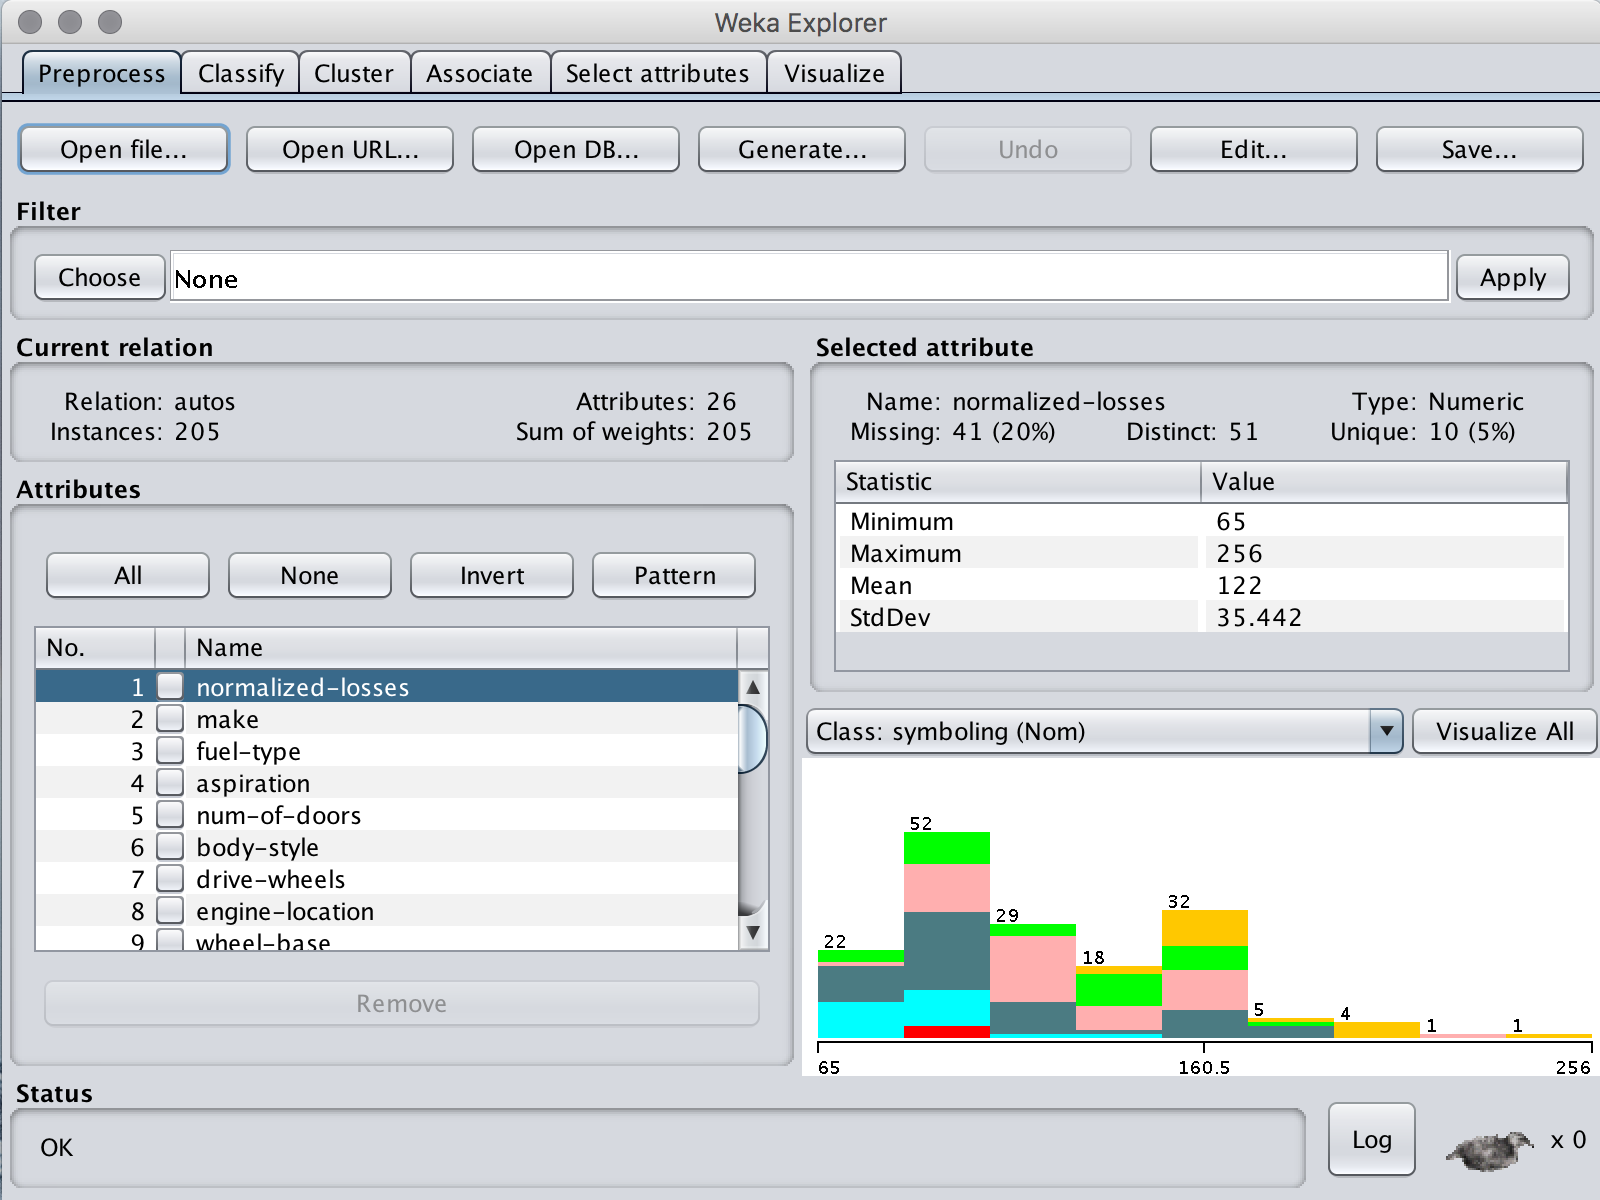
\includegraphics[width=0.9\textwidth]{images/B2_1.png}
\caption{The Explorer interface.}
\label{fig:explorer}
\end{figure}

WEKA's main graphical user interface, the Explorer, gives access to
all its facilities using menu selection and form filling. It is
illustrated in Figure~\ref{fig:explorer}. To begin, there are six
different panels, selected by the tabs at the top, corresponding to
the various data mining tasks that WEKA supports. Further panels can
become available by installing appropriate packages.


\section{Getting started}
\label{sect:getting_started}

Suppose you have some data and you want to build a decision tree from
it. First, you need to prepare the data, then fire up the Explorer and
load in the data. Next you select a decision tree construction method,
build a tree, and interpret the output. It is easy to do it again with
a different tree construction algorithm or a different evaluation
method. In the Explorer you can flip back and forth between the
results you have obtained, evaluate the models that have been built on
different datasets, and visualize graphically both the models and the
datasets themselves---including any classification errors the models
make.

\begin{figure}[!th]
\centering
\subfloat[Spreadsheet.]{\label{subfig:weather_1}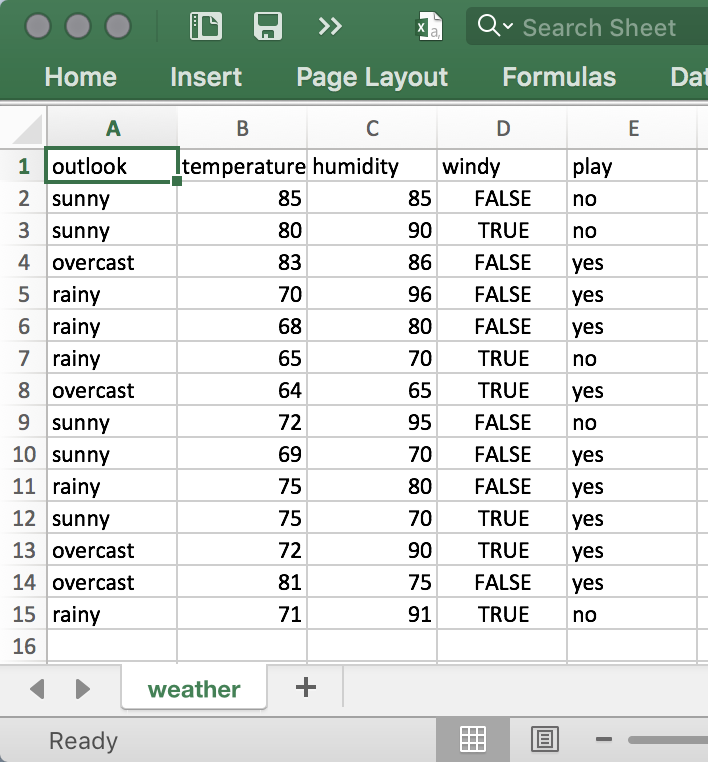
\includegraphics[width=0.45\textwidth]{images/B2_2a.png}}
\qquad
\subfloat[CSV.]{\label{subfig:weather_2}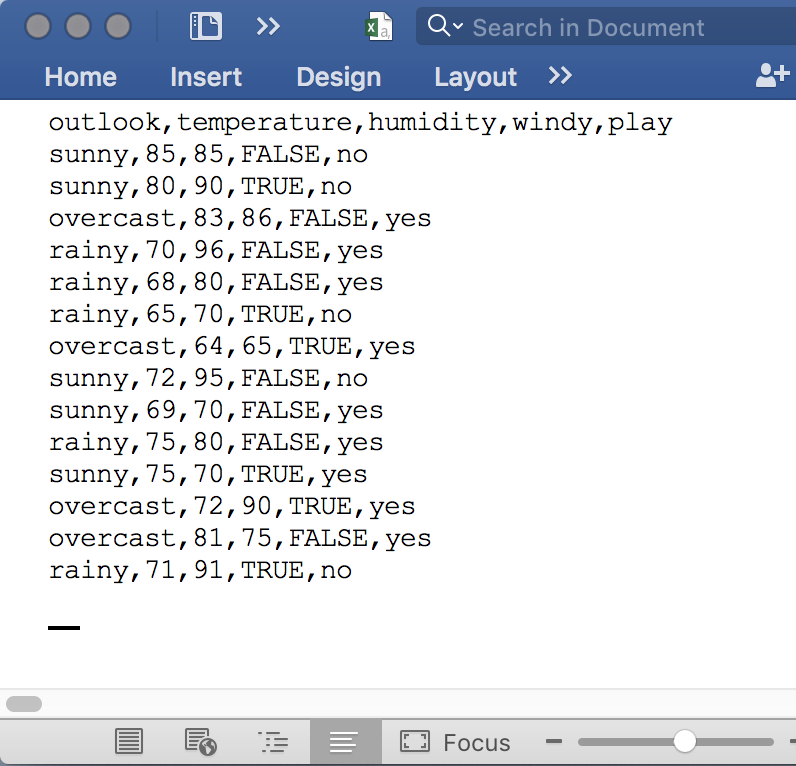
\includegraphics[width=0.45\textwidth]{images/B2_2b.png}}
\newline
\subfloat[ARFF.]{\label{subfig:weather_3}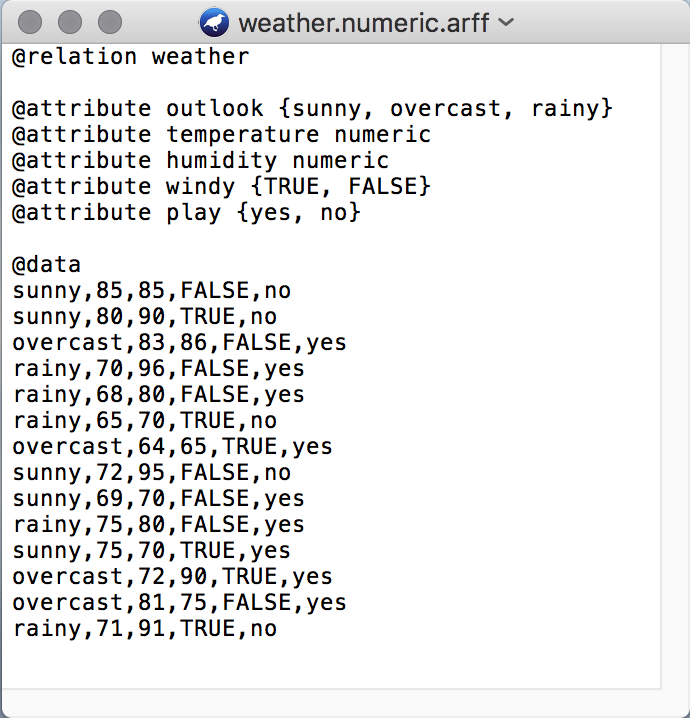
\includegraphics[width=0.45\textwidth]{images/B2_2c.png}}
\caption{\label{fig:weather}Weather data.}
\end{figure}

\subsection{Preparing the data}

The data is often presented in a spreadsheet or database. However,
WEKA's native data storage method is ARFF format. You can easily
convert from a spreadsheet to ARFF. The bulk of an ARFF file consists
of a list of the instances, and the attribute values for each instance
are separated by commas. Most spreadsheet and database programs allow
you to export data into a file in comma-separated value (CSV) format
as a list of records with commas between items. Having done this, you
need only load the file into a text editor or word processor; add the
dataset's name using the @relation tag, the attribute information
using @attribute, and a @data line; and save the file as raw text. For
example, Figure~\ref{fig:weather} shows an Excel spreadsheet
containing the weather data, the data in CSV form loaded into
Microsoft Word, and the result of converting it manually into an ARFF
file. However, you do not actually have to go through these steps to
create the ARFF file yourself, because the Explorer can read CSV
spreadsheet files directly, as described later.

\subsection{Loading the data into the Explorer}

\begin{figure}[!th]
\centering
\subfloat[Choosing the Explorer interface.]{\label{subfig:explorer_1}
\includegraphics[width=0.3\textwidth]{images/B2_3a.png}}
\qquad
\subfloat[Reading in the weather data.]{\label{subfig:explorer_2}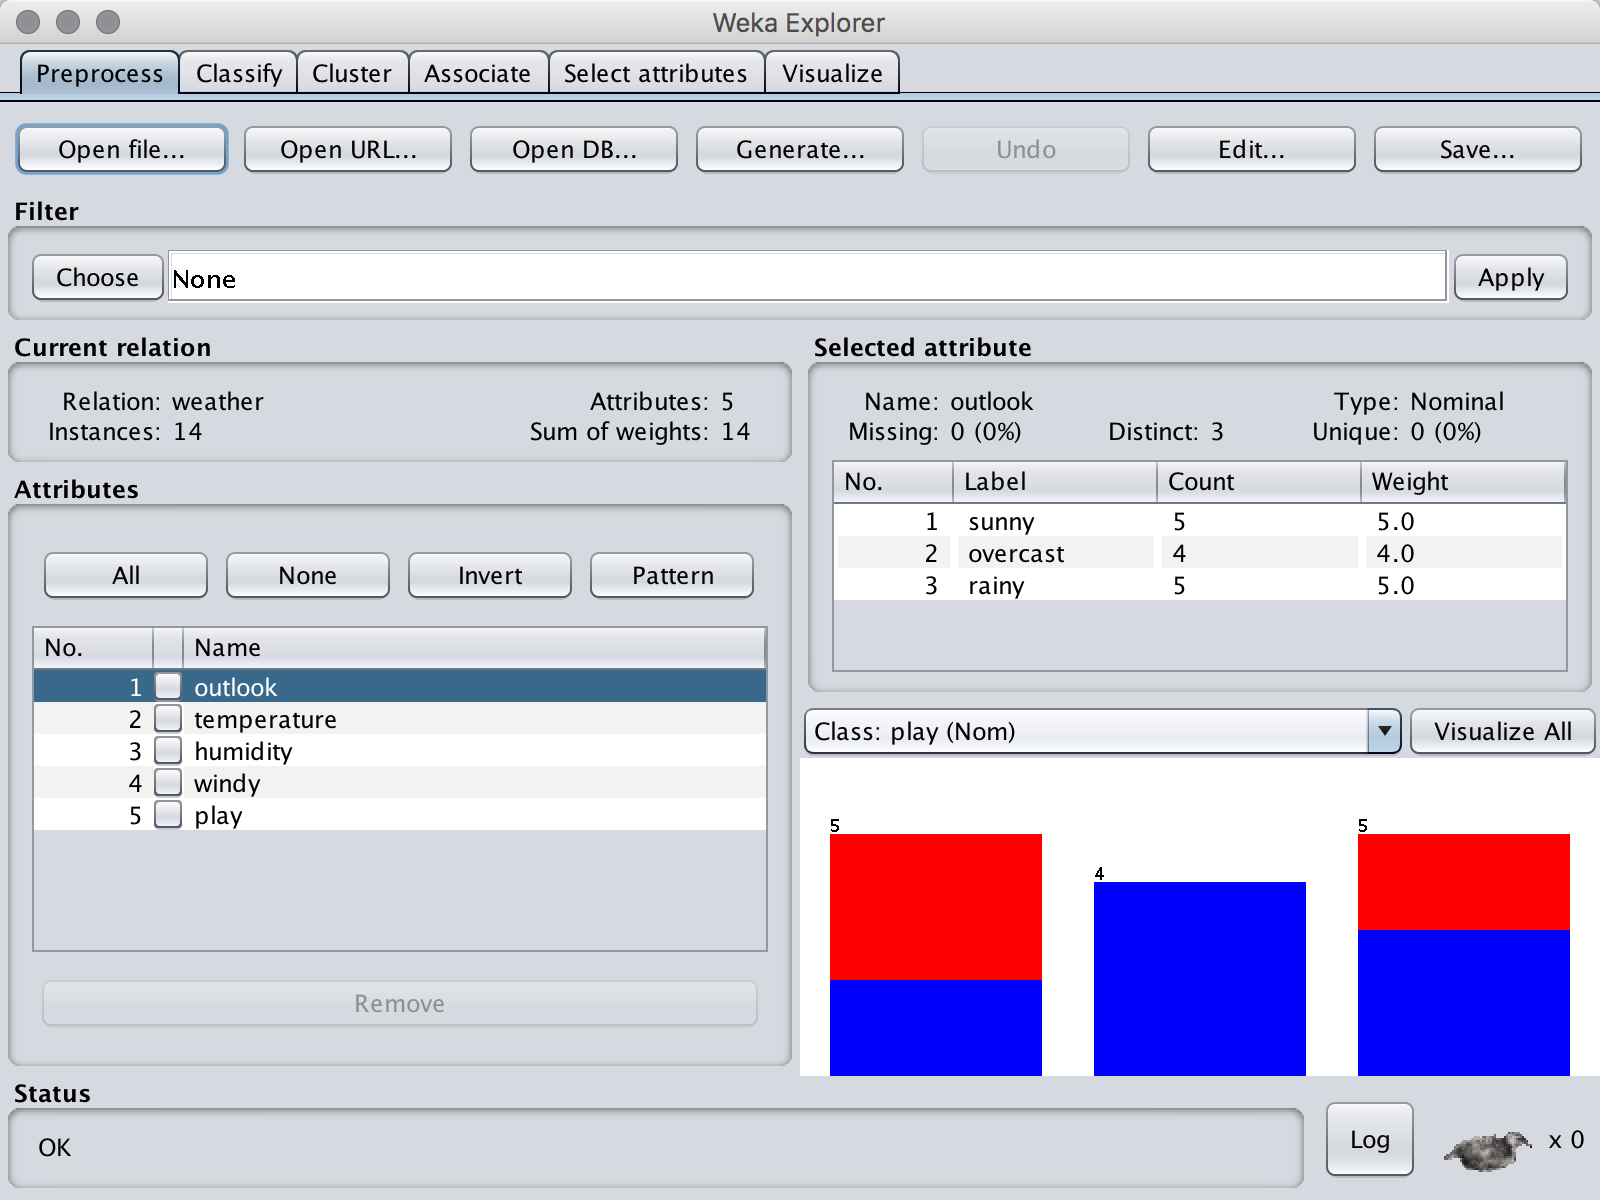
\includegraphics[width=0.6\textwidth]{images/B2_3b.png}}
\caption{\label{fig:weather_explorer}Weather data in the Explorer.}
\end{figure}

Let us load this data into the Explorer and start analyzing it. Fire up
WEKA to get the \textit{GUI Chooser panel} in Figure~\ref{subfig:explorer_1}. Select
\textit{Explorer} from the five choices on the right-hand side. (The
others were mentioned earlier: \textit{Simple CLI} is the
old-fashioned command-line interface.)

What you see next is the main Explorer screen, shown in
Figure~\ref{subfig:explorer_2}. Actually, the figure shows what it will
look like \textit{after} you have loaded in the weather data. The six
tabs along the top are the basic operations that the Explorer
supports: right now we are on \textit{Preprocess}. Click the Open file
button to bring up a standard dialog through which you can select a
file. Choose the \textit{weather.arff} file. If you have it in CSV
format, change from \textit{ARFF data files} to \textit{CSV data
  files}. When you specify a .csv file it is automatically converted
into ARFF format.

Having loaded the file, the screen will be as shown in
Figure~\ref{subfig:explorer_2}. This tells you about the dataset: it
has 14 instances and five attributes (center left); the attributes are
called \textit{outlook}, \textit{temperature}, \textit{humidity},
\textit{windy}, and \textit{play} (lower left). The first attribute,
\textit{outlook}, is selected by default (you can choose others by
clicking them) and has no missing values, three distinct values, and
no unique values; the actual values are \textit{sunny},
\textit{overcast}, and \textit{rainy} and they occur five, four, and
five times, respectively (center right). A histogram at the lower
right shows how often each of the two values of the class,
\textit{play}, occurs for each value of the \textit{outlook}
attribute. The attribute \textit{outlook} is used because it appears
in the box above the histogram, but you can draw a histogram of any
other attribute instead. Here \textit{play} is selected as the class
attribute; it is used to color the histogram, and any filters that
require a class value use it too.

The \textit{outlook} attribute in Figure~\ref{subfig:explorer_2} is
nominal. If you select a numeric attribute, you see its minimum and
maximum values, mean, and standard deviation. In this case the
histogram will show the distribution of the class as a function of
this attribute.

You can delete an attribute by clicking its checkbox and using the
\textit{Remove} button. \textit{All} selects all the attributes,
\textit{None} selects none, Invert \textit{inverts} the current
selection, and \textit{Pattern} selects those attributes whose names
match a user-supplied regular expression. You can undo a change by
clicking the \textit{Undo} button. The \textit{Edit} button brings up
an editor that allows you to inspect the data, search for particular
values and edit them, and delete instances and
attributes. Right-clicking on values and column headers brings up
corresponding context menus.

\subsection{Building a decision tree}
\label{subsection:building_decision_tree}

\begin{figure}[!th]
\centering
\subfloat[Finding J4.8 in the classifiers list.]{\label{subfig:j48_1}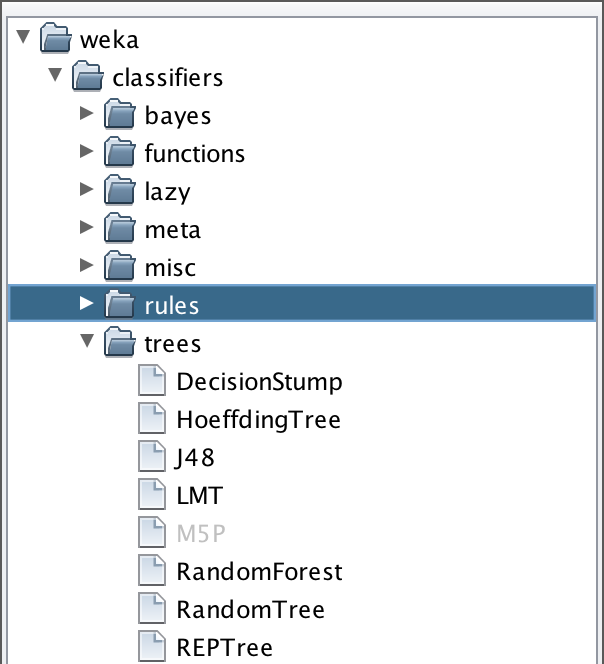
\includegraphics[width=0.3\textwidth]{images/B2_4a.png}}
\qquad
\subfloat[The \textit{Classify} tab.]{\label{subfig:j48_2}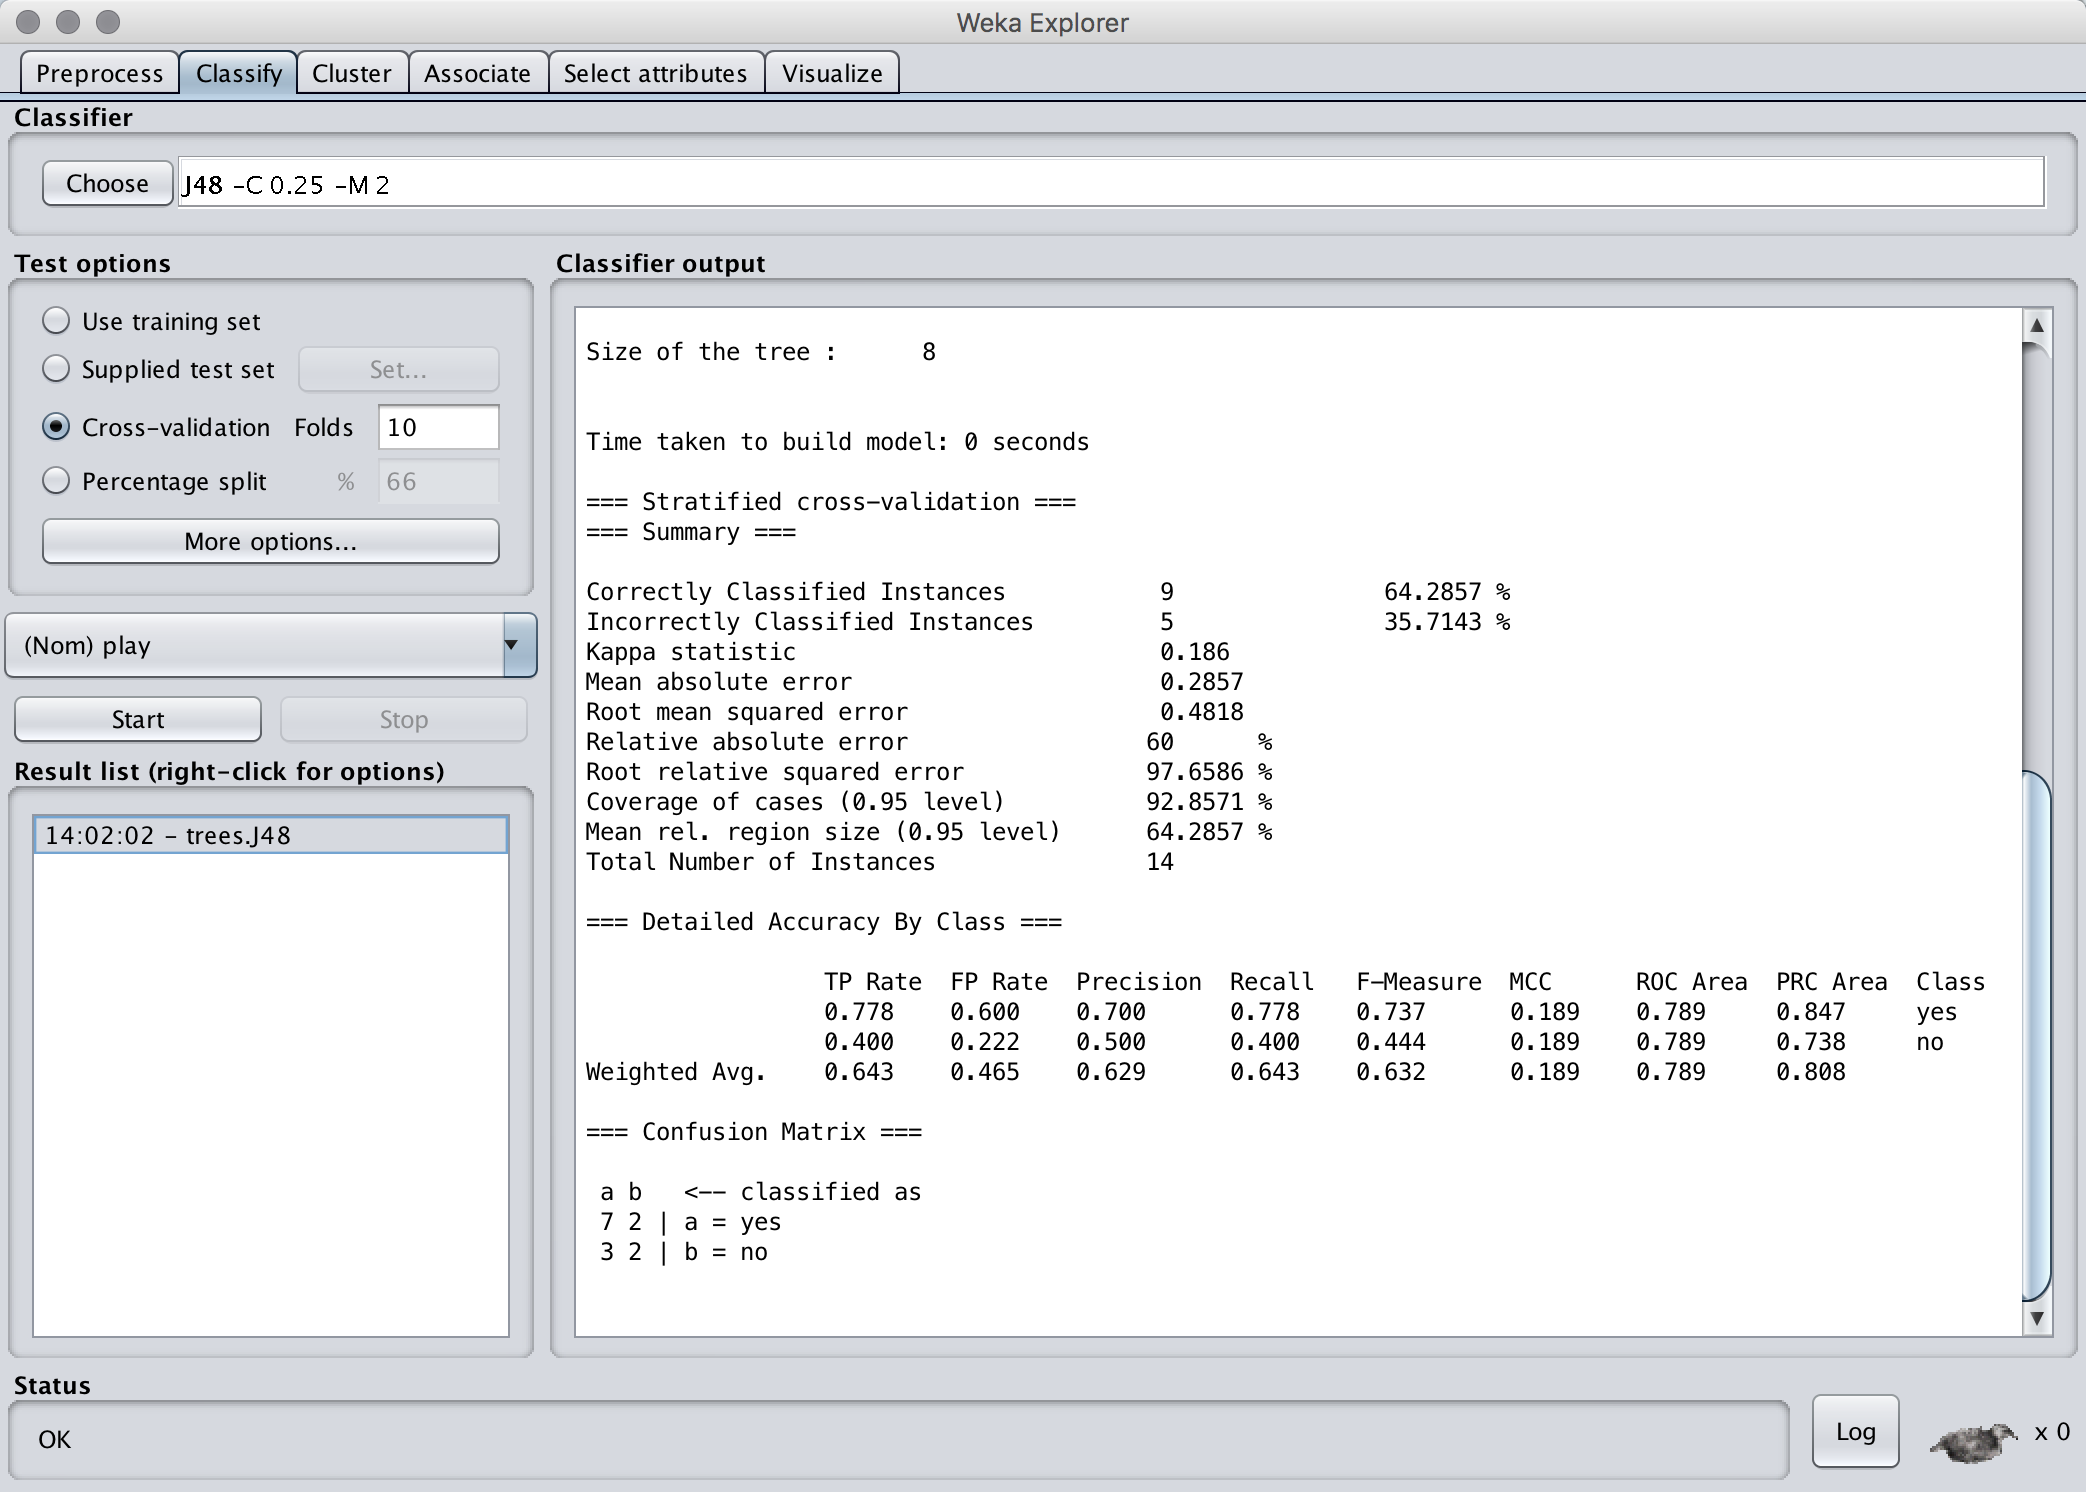
\includegraphics[width=0.6\textwidth]{images/B2_4b.png}}
\caption{\label{fig:j48_explorer}J4.8 in the Explorer.}
\end{figure}

To see what the C4.5 decision tree learner does with this dataset, use
the J4.8 algorithm, which is WEKA's implementation of this
algorithm. (J4.8 actually implements a later and slightly improved
version called C4.5 revision 8, which was the last public version of
this family of algorithms before C5.0 was released.) Click the
\textit{Classify} tab to get a screen that looks like
Figure~\ref{subfig:j48_2}. Actually, the figure shows what it will
look like \textit{after} you have analyzed the weather data.

First select the classifier by clicking the \textit{Choose} button at
the top left, opening up the trees section of the hierarchical menu in
Figure~\ref{subfig:j48_1}, and finding \textit{J48}. The menu
structure represents the organization of the WEKA code into modules
and the items you need to select are always at the lowest level. Once
selected, \textit{J48} appears in the line beside the \textit{Choose}
button as shown in Figure~\ref{subfig:j48_2}, along with its default parameter
values. If you click that line, the J4.8 classifier's object editor
opens up and you can see what the parameters mean and alter their
values if you wish. The Explorer generally chooses sensible defaults.

Having chosen the classifier, invoke it by clicking the \textit{Start}
button. WEKA works for a brief period---when it is working, the little
bird at the lower right of Figure 2.4b jumps up and dances---and then
produces the output shown in the main panel of
Figure~\ref{subfig:j48_2}.

\subsection{Examining the output}

\begin{figure}[!th]
%\centering
\begin{mdframed}[innermargin=-1cm]
\begin{Verbatim}[fontsize=\footnotesize]
=== Run information ===

Scheme:       weka.classifiers.trees.J48 -C 0.25 -M 2
Relation:     weather
Instances:    14
Attributes:   5
              outlook
              temperature
              humidity
              windy
              play
Test mode:    10-fold cross-validation

=== Classifier model (full training set) ===

J48 pruned tree
------------------

outlook = sunny
|   humidity <= 75: yes (2.0)
|   humidity > 75: no (3.0)
outlook = overcast: yes (4.0)
outlook = rainy
|   windy = TRUE: no (2.0)
|   windy = FALSE: yes (3.0)

Number of Leaves  : 5

Size of the tree : 8

Time taken to build model: 0.27 seconds

=== Stratified cross-validation ===
=== Summary ===

Correctly Classified Instances           9               64.2857 %
Incorrectly Classified Instances         5               35.7143 %
Kappa statistic                          0.186 
Mean absolute error                      0.2857
Root mean squared error                  0.4818
Relative absolute error                 60      %
Root relative squared error             97.6586 %
Total Number of Instances               14     

=== Detailed Accuracy By Class ===

               TP Rate   FP Rate   Precision   Recall  F-Measure   ROC Area  Class
                 0.778     0.6        0.7       0.778     0.737      0.789    yes
                 0.4       0.222      0.5       0.4       0.444      0.789    no
Weighted Avg.    0.643     0.465      0.629     0.643     0.632      0.789

=== Confusion Matrix ===

 a b   <-- classified as
 7 2 | a = yes
 3 2 | b = no
\end{Verbatim}
\end{mdframed}
\caption{\label{fig:j48_output}Output from the J4.8 decision tree learner.}
\end{figure}

Figure 2.5 shows the full output (Figure~\ref{subfig:j48_2} only gives
the lower half). At the beginning is a summary of the dataset, and the
fact that 10-fold cross-validation was used to evaluate it. That is
the default, and if you look closely at Figure~\ref{subfig:j48_2} you
will see that the \textit{Cross-validation} box at the left is
checked. Then comes a pruned decision tree in textual form. The model
that is shown here is always one generated from the full dataset
available from the \textit{Preprocess panel}. The first split is on
the outlook attribute, and then, at the second level, the splits are
on humidity and windy, respectively. In the tree structure, a colon
introduces the class label that has been assigned to a particular
leaf, followed by the number of instances that reach that leaf,
expressed as a decimal number because of the way the algorithm uses
fractional instances to handle missing values. If there were
incorrectly classified instances (there aren't in this example) their
number would appear too: thus \textit{2.0/1.0} means that two
instances reached that leaf, of which one is classified
incorrectly. Beneath the tree structure the number of leaves is
printed; then the total number of nodes (\textit{Size of the
  tree}). There is a way to view decision trees more graphically,
which we will encounter later.

%% Fix the reference above to page 484

The next part of the output gives estimates of the tree's predictive
performance. In this case they are obtained using stratified
cross-validation with 10 folds, the default in
Figure~\ref{subfig:j48_2}. As you can see, more than 30\% of the
instances (5 out of 14) have been misclassified in the
cross-validation. This indicates that the results obtained from the
training data are optimistic compared with what might be obtained from
an independent test set from the same source. From the confusion
matrix at the end observe that 2 instances of class \textit{yes} have
been assigned to class \textit{no} and 3 of class \textit{no} are
assigned to class \textit{yes}.

As well as the classification error, the evaluation module also
outputs the Kappa statistic, the mean absolute error, and the root
mean-squared error of the class probability estimates assigned by the
tree. The root mean-squared error is the square root of the average
squared loss. The mean absolute error is calculated in a similar way
using the absolute instead of the squared difference. It also outputs
relative errors, which are based on the prior probabilities (i.e.,
those obtained by the ZeroR learning scheme described later). Finally,
for each class it also outputs various statistics. Also reported is
the per-class average of each statistic, weighted by the number of
instances from each class. All of these evaluation measures are
discussed in Chapter 5 of the book.

\subsection{Doing it again}
\label{subsec:doing_it_again}

You can easily run J4.8 again with a different evaluation
method. Select {\em Use training set} (near the top left in
Figure~\ref{subfig:j48_2}) and click \textit{Start} again. The
classifier output is quickly replaced to show how well the derived
model performs on the training set, instead of showing the
cross-validation results. This evaluation is highly optimistic. It may
still be useful, because it generally represents an upper bound to the
model's performance on fresh data. In this case, all 14 training
instances are classified correctly. In some cases a classifier may
decide to leave some instances unclassified, in which case these will
be listed as \textit{Unclassified Instances}. This does not happen for
most learning schemes in WEKA.

The panel in Figure~\ref{subfig:j48_2} has further test options:
\textit{Supplied test set}, in which you specify a separate file
containing the test set, and \textit{Percentage split}, with which you
can hold out a certain percentage of the data for testing. You can
output the predictions for each instance by clicking the \textit{More
  options} button and checking the appropriate entry. There are other
useful options, such as suppressing some output and including other
statistics such as entropy evaluation measures and cost-sensitive
evaluation. For the latter you must enter a cost matrix: type the
number of classes into the \textit{Classes} box (and terminate it with
the \textit{Enter} or \textit{Return} key) to get a default cost
matrix, then edit the values as required.

\subsection{Working with models}

The small pane at the lower left of Figure~\ref{subfig:j48_2}, which
contains one highlighted line, is a history list of the results. The
Explorer adds a new line whenever you run a classifier. Because you
have now run the classifier twice, the list will contain two items. To
return to a previous result set, click the corresponding line and the
output for that run will appear in the Classifier Output pane. This
makes it easy to explore different classifiers or evaluation schemes
and revisit the results to compare them.

The result history list is the entry point to some powerful features
of the Explorer. When you \textit{right}-click an entry a menu appears that
allows you to view the results in a separate window, or save the
result buffer. More importantly, you can save the model that WEKA has
generated in the form of a Java object file. You can reload a model
that was saved previously, which generates a new entry in the result
list. If you now supply a test set, you can reevaluate the old model
on that new set.

Several items on the right-click menu allow you to visualize the
results in various ways. At the top of the Explorer interface is a
separate \textit{Visualize} tab, but that is different: it shows the
dataset, not the results for a particular model. By right-clicking an
entry in the history list you can see the classifier errors. If the
model is a tree or a Bayesian network you can see its structure. You
can also view the margin curve and various cost and threshold curves,
including the cost/benefit analysis tool. For all of these you must
choose a class value from a submenu. The \textit{Visualize threshold
  curve} menu item allows you to see the effect of varying the
probability threshold above which an instance is assigned to that
class. You can select from a wide variety of curves that include the
ROC and recall-precision curves. To see these, choose the X- and
Y-axes appropriately from the menus given. For example, set X to
\textit{False Positive Rate} and Y to \textit{True Positive Rate} for
an ROC curve or X to \textit{Recall} and Y to \textit{Precision} for a
recall-precision curve.

\begin{figure}[!th]
\centering
\subfloat[\textit{J4.8} tree for the iris data.]{\label{subfig:j48_3}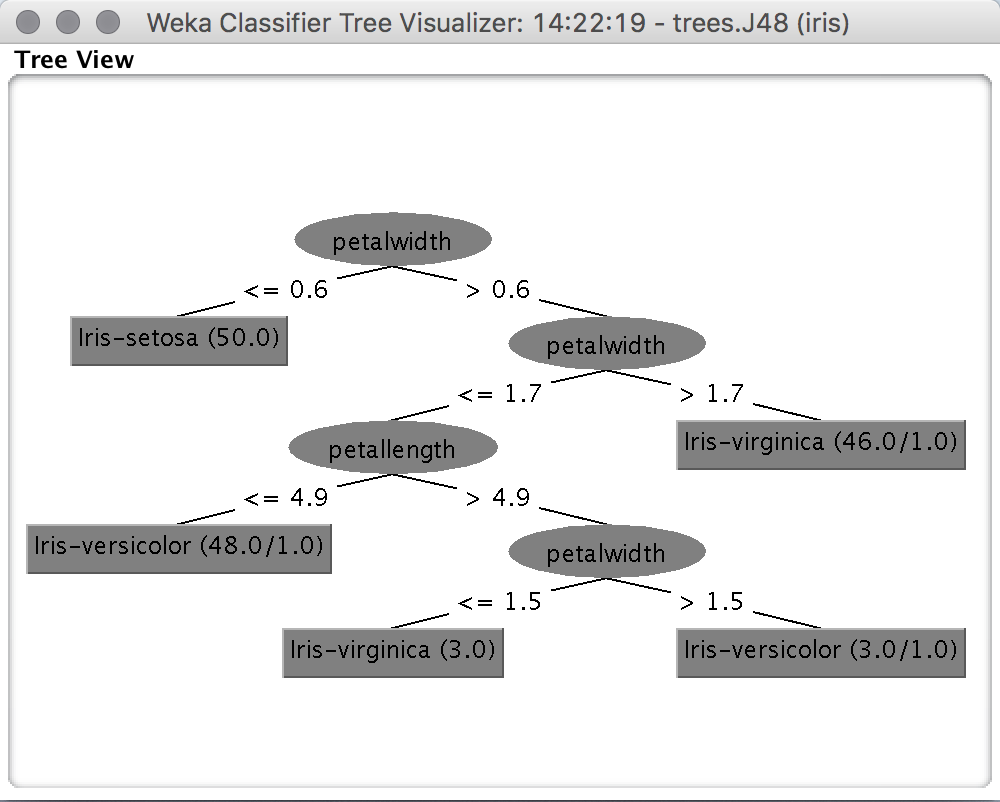
\includegraphics[width=0.9\textwidth]{images/B2_6a.png}}
\newline
\subfloat[\textit{J4.8}'s errors on the iris data.]{\label{subfig:j48_4}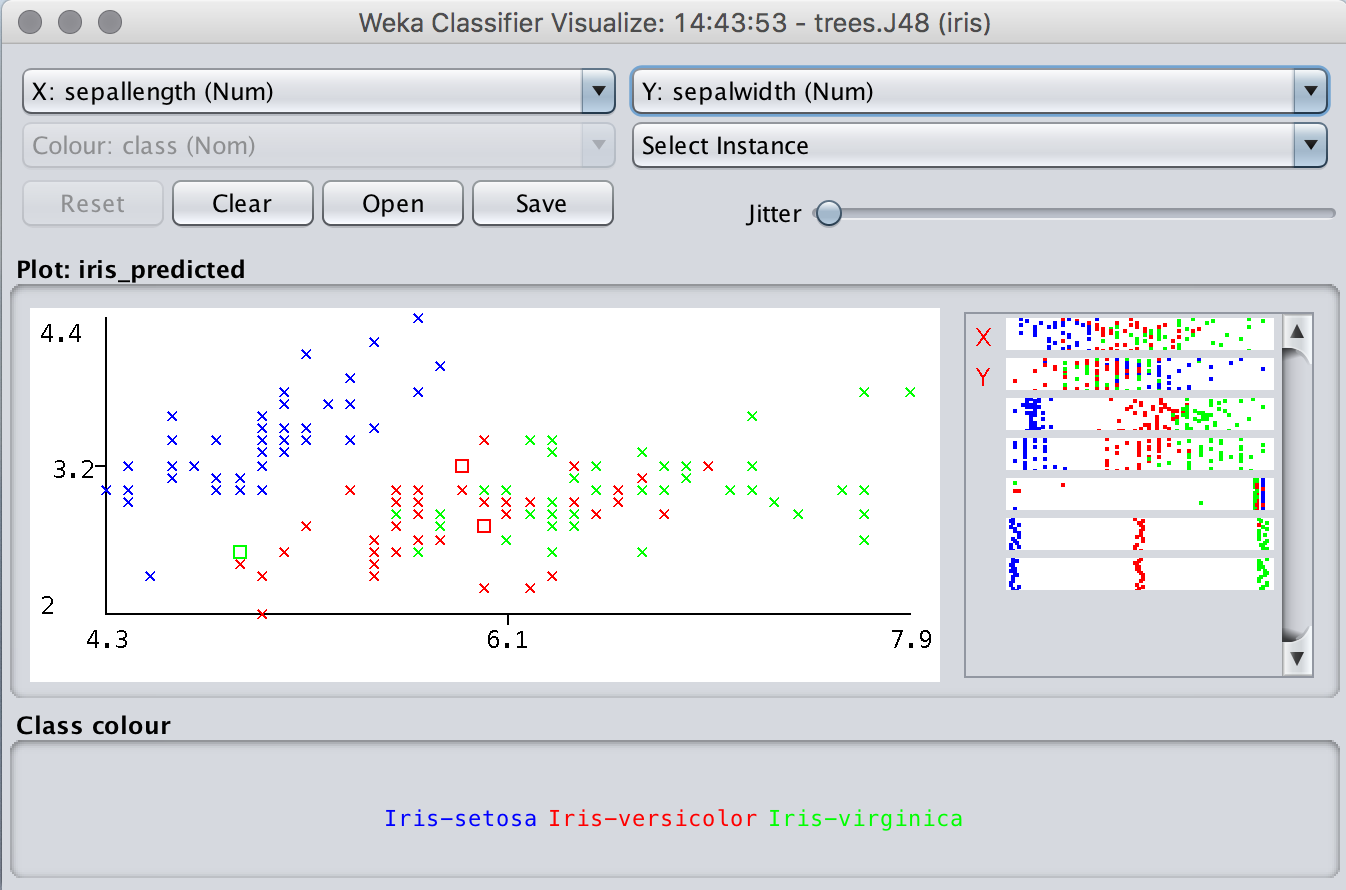
\includegraphics[width=0.9\textwidth]{images/B2_6b.png}}
\caption{\label{fig:j48_iris}Visualizing the result of \textit{J4.8} on the iris data.}
\end{figure}

Figure~\ref{fig:j48_iris} shows two ways of looking at the result of
using J4.8 to classify the iris dataset---we use this rather than the
weather data because it produces more interesting
pictures. Figure~\ref{subfig:j48_3} shows the tree. Right-click a
blank space in this window to bring up a menu enabling you to
automatically scale the view or force the tree into the window. Drag
the mouse to pan around the space. It's also possible to visualize the
instance data at any node, if it has been saved by the learning
algorithm.

Figure~\ref{subfig:j48_4} shows the classifier errors on a
two-dimensional plot. You can choose which attributes to use for X and
Y using the selection boxes at the top. Alternatively, click one of
the speckled horizontal strips to the right of the plot: left-click
for X and right-click for Y. Each strip shows the spread of instances
along that attribute. X and Y appear beside the ones you have chosen
for the axes.

The data points are colored according to their class: blue, red and
green for \textit{Iris setosa}, \textit{Iris versicolor}, and
\textit{Iris virginica}, respectively (there is a key at the bottom of
the screen). Correctly classified instances are shown as crosses;
incorrectly classified ones appear as boxes (of which there are three
in Figure~\ref{subfig:j48_4}). You can click on an instance to bring
up relevant details: its instance number, the values of the
attributes, its class, and the predicted class.

\subsection{When things go wrong}

Beneath the result history list, at the bottom of
Figure~\ref{subfig:explorer_2}, is a status line that says, simply,
\textit{OK}. Occasionally this changes to \textit{See error log}, an
indication that something has gone wrong. For example, there may be
constraints among the various different selections you can make in a
panel. Most of the time the interface grays out inappropriate
selections and refuses to let you choose them. But occasionally the
interactions are more complex, and you can end up selecting an
incompatible set of options. In this case, the status line changes
when WEKA discovers the incompatibility---typically when you press
\textit{Start}. To see the error, click the \textit{Log} button to the
left of the bird in the lower right-hand corner of the interface. WEKA
also writes a detailed log to a file, called \textit{weka.log}, under
the \textit{wekafiles} directory in the user's home directory. This
often contains more information about the causes of problems than the
Explorer's Log window because it captures debugging output directed to
the standard out and error channels.

\section{Exploring the Explorer}
\label{section:exploring_the_explorer}

We have briefly investigated two of the six tabs at the top of the
Explorer window in Figure~\ref{subfig:explorer_2} and
Figure~\ref{subfig:j48_2}. In summary, here's what all of the tabs do:

\begin{enumerate}
\item \textit{Preprocess}: Choose the dataset and modify it in various ways.
\item \textit{Classify}: Train learning schemes that perform classification or regression and evaluate them.
\item \textit{Cluster}: Learn clusters from the dataset.
\item \textit{Associate}: Learn association rules for the data and evaluate them.
\item \textit{Select attributes}: Select the most relevant aspects of the dataset.
\item \textit{Visualize}: View different two-dimensional plots of the data and interact with them.
\end{enumerate}

Each tab gives access to a whole range of facilities. In our tour so
far, we have barely scratched the surface of the \textit{Preprocess}
and \textit{Classify} panels.

At the bottom of every panel is a \textit{Status} box and a
\textit{Log} button. The status box displays messages that keep you
informed about what's going on. For example, if the Explorer is busy
loading a file, the status box will say so. Right-clicking anywhere
inside this box brings up a little menu with two options: display the
amount of memory available to WEKA, and run the Java garbage
collector. Note that the garbage collector runs constantly as a
background task anyway.

Clicking the \textit{Log} button opens a textual log of the actions that WEKA
has performed in this session, with timestamps.

As noted earlier, the little bird at the lower right of the window
jumps up and dances when WEKA is active. The number beside the $\times$
shows how many concurrent processes are running. If the bird is
standing but stops moving, it's sick! Something has gone wrong, and
you may have to restart the Explorer.

\subsection{Loading and filtering files}

Along the top of the \textit{Preprocess panel} in
Figure~\ref{subfig:explorer_2} are buttons for opening files, URLs,
and databases. Initially, only files whose names end in \textit{.arff}
appear in the file browser; to see others, change the \textit{Format}
item in the file selection box.

\subsection{Converting files to ARFF}

WEKA has converters for the following file formats: 

\begin{itemize}
\item spreadsheet files with extension \textit{.csv},
\item C4.5's native file format with extensions \textit{.names} and \textit{.data},
\item serialized instances with extension \textit{.bsi},
\item LIBSVM format files with extension \textit{.libsvm},
\item SVM-Light format files with extension \textit{.dat},
\item XML-based ARFF format files with extension \textit{.xrff},
\item JSON-based ARFF format files with extension \textit{.json},
\item ASCII Matlab files with extension \textit{.m}.
\end{itemize}

\begin{figure}[!th]
\centering
\subfloat[Generic Object Editor.]{\label{subfig:goe_1}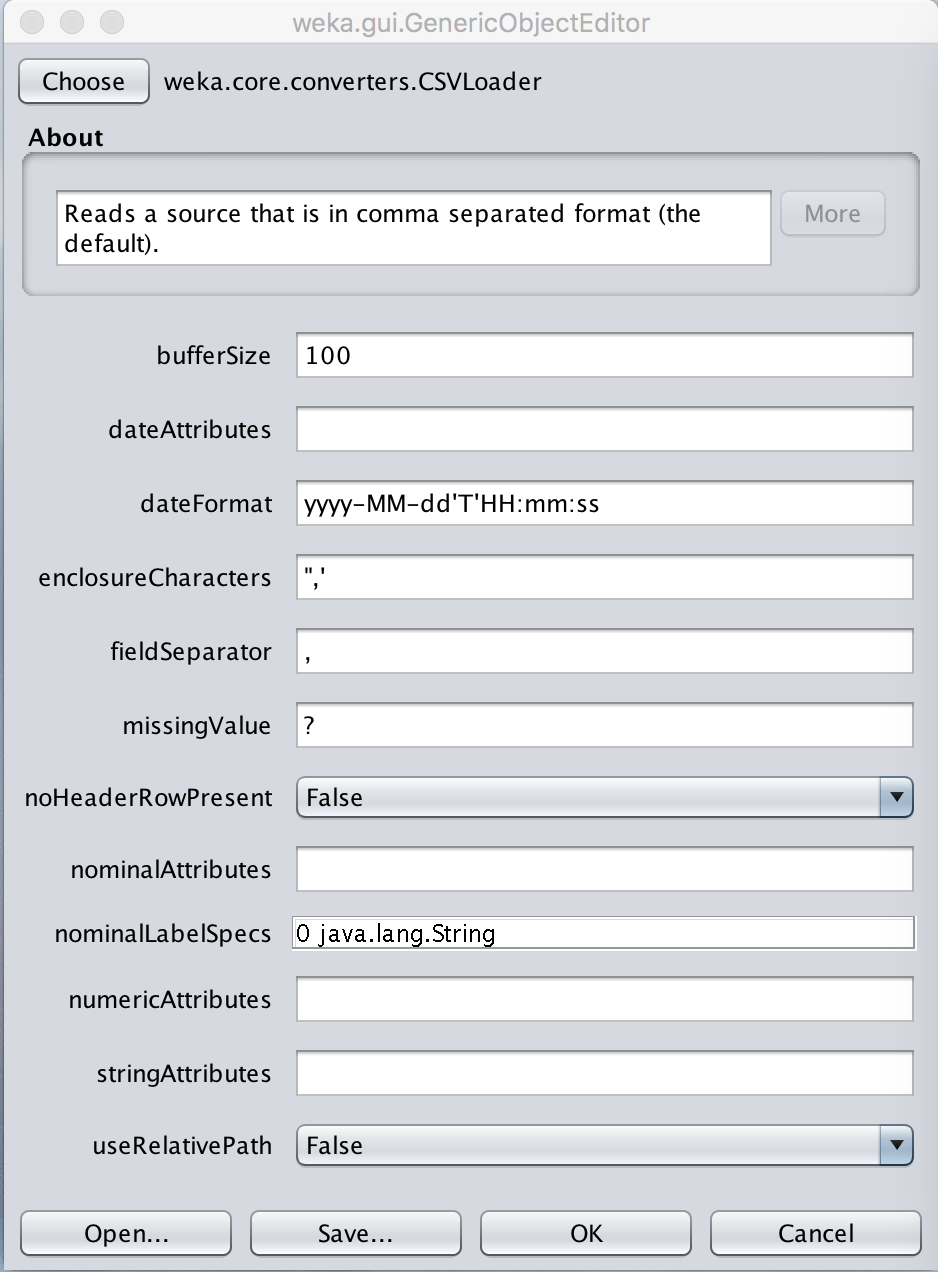
\includegraphics[width=0.45\textwidth]{images/B2_7a.png}}
\qquad
\subfloat[More information.]{\label{subfig:goe_2}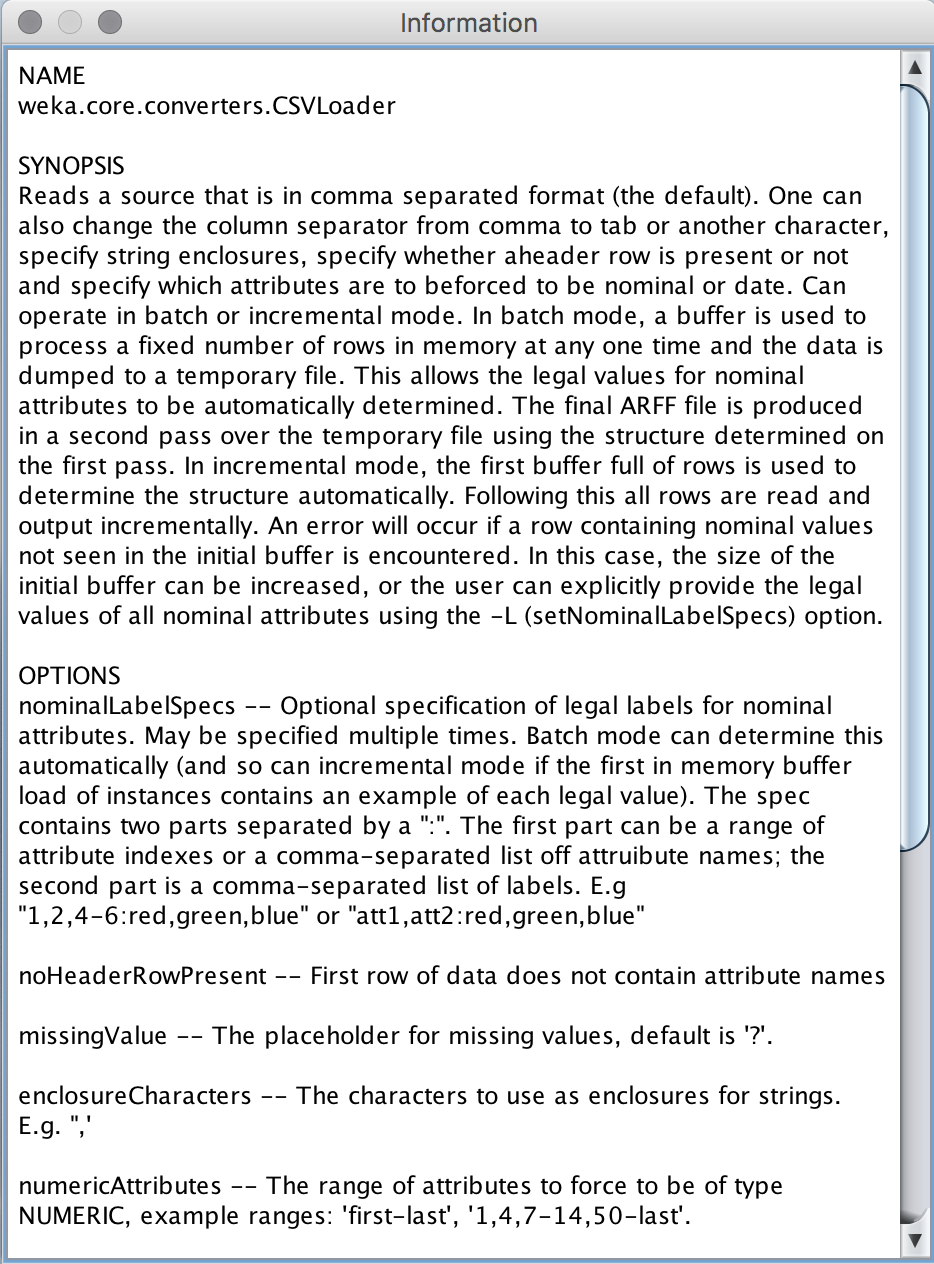
\includegraphics[width=0.45\textwidth]{images/B2_7b.png}}
\newline
\subfloat[Choosing a converter (click Choose).]{\label{subfig:goe_3}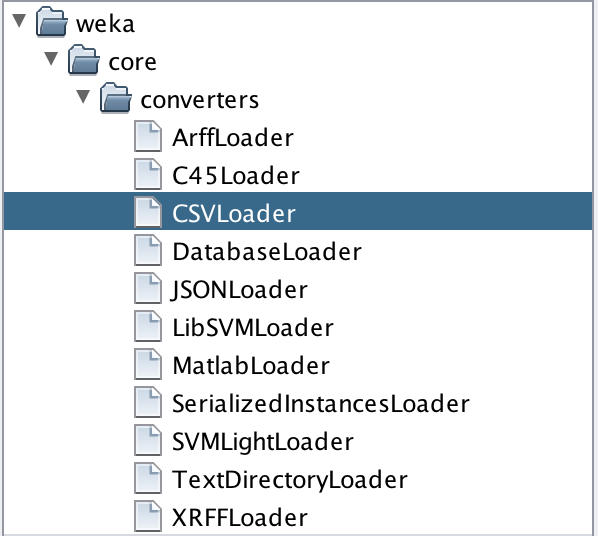
\includegraphics[width=0.45\textwidth]{images/B2_7c.png}}
\caption{\label{fig:goe}The Generic Object Editor.}
\end{figure}

The appropriate converter is used based on the file extension. If WEKA
cannot load the data, it tries to interpret it as ARFF. If that fails,
it pops up the box shown in Figure~\ref{subfig:goe_1}.

This is a generic object editor, used throughout WEKA for selecting
and configuring object. For example, when you set parameters for a
classifier, you use the same kind of box. The \textit{CSVLoader} for
\textit{.csv} files is selected by default, and the \textit{More}
button gives you more information about it, shown in
Figure~\ref{subfig:goe_2}. It is always worth looking at the
documentation! In this case, it explains that the spreadsheet's first
row determines the attribute names and gives a brief description of
the CSVLoader's options. Click \textit{OK} to use this converter. For
a different one, click \textit{Choose} to select from the list in
Figure~\ref{subfig:goe_3}.

\begin{figure}[!th]
\centering
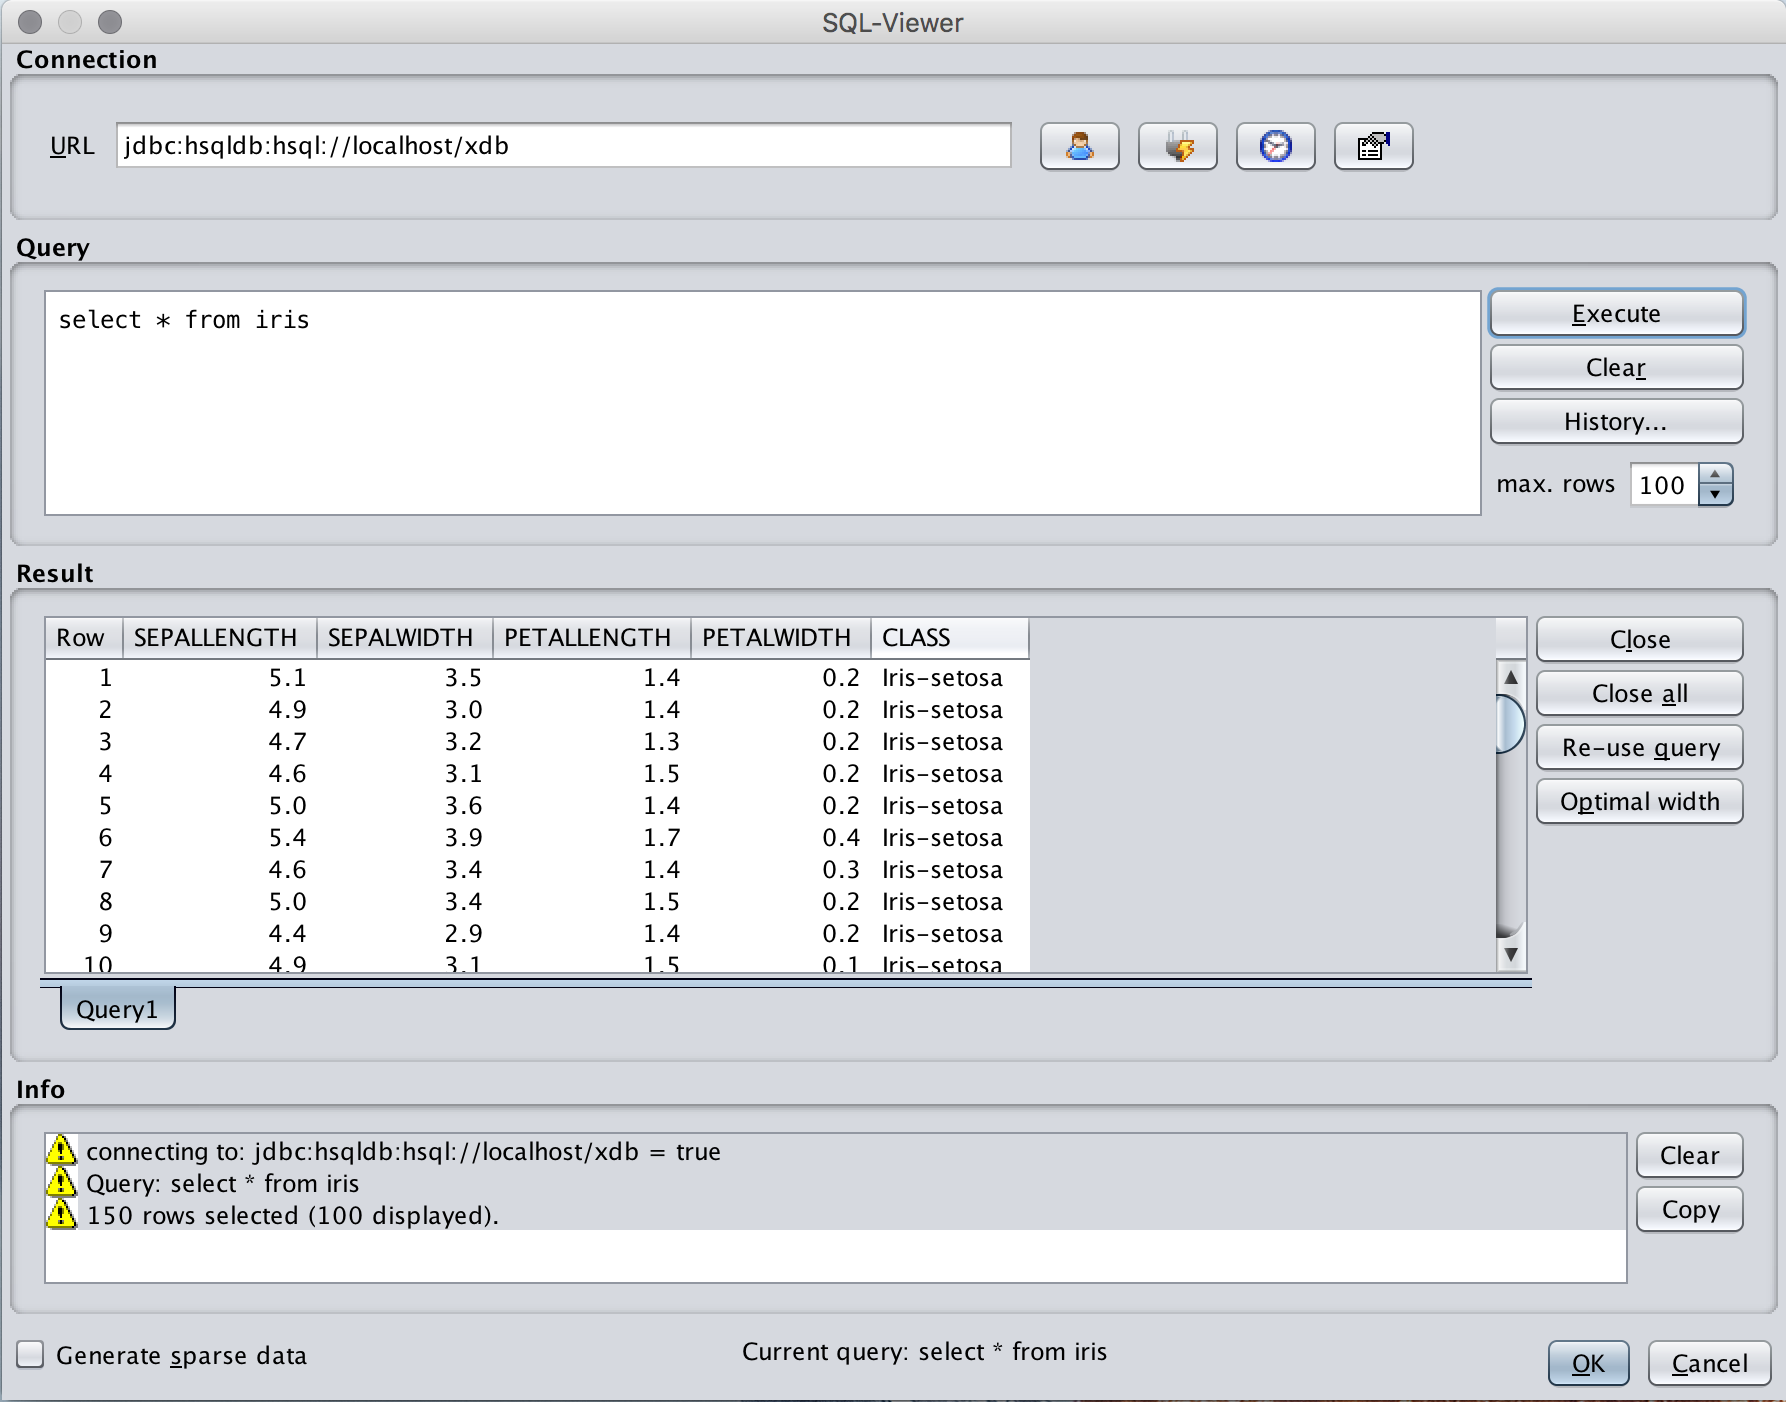
\includegraphics[width=0.9\textwidth]{images/B2_8.png}
\caption{The SQLViewer tool.}
\label{fig:sql_viewer}
\end{figure}


The \textit{ArffLoader} is the first option, and we reached this point
only because it failed. The second option is for the C4.5 format, in
which there are two files for a dataset, one giving field names and
the other giving the actual data. The third option,
\textit{CSVLoader}, is the default, and we clicked \textit{Choose}
because we want a different one. The fourth option is for reading from
a database rather than a file; however, the \textit{SQLViewer} tool,
shown in Figure~\ref{fig:sql_viewer} and accessible by pressing the \textit{Open DB}
button on the \textit{Preprocess} panel, is a more user-friendly route
for accessing a database. The ``serialized instances'' option is for
reloading datasets that have been saved as Java serialized object. Any
Java object can be saved in this format and reloaded. As a native Java
format, it is quicker to load that an ARFF file, which must be parsed
and checked. When repeatedly reloading a large dataset it may be worth
saving it in this form.

The tenth menu item is for importing a directory containing plain text
files for the purposes of text mining. The imported directory is
expected to have a specific structure---namely a set of
subdirectories, each containing one or more text files with the
extension \textit{.txt}. Each text file becomes one instance in the
dataset, with a string attribute holding the contents of the file and
a nominal class attribute holding the name of the subdirectory that it
came from. This dataset can then be further processed into word
frequencies using the \textit{StringToWordVector} filter (covered in
the next section). The last option is for loading data files in XRFF,
the XML Attribute Relation File format. As the name suggests, this
gives ARFF header and instance information in the XML markup language.

Further features of the generic object editor in Figure~\ref{subfig:goe_1} are
\textit{Save}, which saves a configured object, and \textit{Open},
which opens a previously saved one. These are not useful for this
particular kind of object. But other generic object editor panels have
many editable properties, and having gone to some trouble to set them
up you may want to save the configured object to reuse later.

Files on your computer are not the only source of datasets for
WEKA. You can open a URL, and WEKA will use the hypertext transfer
protocol (HTTP) to download an ARFF file from the Web. Or you can open
a database (Open DB)---any database that has a Java database
connectivity (JDBC) driver---and retrieve instances using the SQL
\textit{Select} statement. This returns a relation that WEKA reads in
as an ARFF file. To make this work with your database, you may need to
modify the file \textit{weka/experiment/DatabaseUtils.props} in the
WEKA distribution by adding your database driver to it. (To access
this file, expand the weka.jar file in the WEKA distribution.)
Figure~\ref{fig:sql_viewer} shows the SQLViewer tool that appears when
\textit{Open DB} is clicked. In this example, the iris dataset has been
extracted from a single database table.

Data can be saved in all these formats (with the exception of the
directory containing text files) using the Save button in the
\textit{Preprocess} panel (Figure~\ref{subfig:explorer_2}). It is also
possible to generate artificial data using the \textit{Generate}
button. Artificial data suitable for classification can be generated
from decision lists, radial-basis function networks and Bayesian
networks, as well as the classic LED24 domain. Artificial regression
data can be generated according to mathematical expressions. There are
also several generators for producing artificial data for clustering
purposes. Apart from loading and saving datasets, the
\textit{Preprocess} panel also allows you to filter them. Filters are
an important component of WEKA.

\subsection{Using filters}

\begin{figure}[!p]
\centering
\subfloat[The filters menu.]{\label{subfig:filters_1}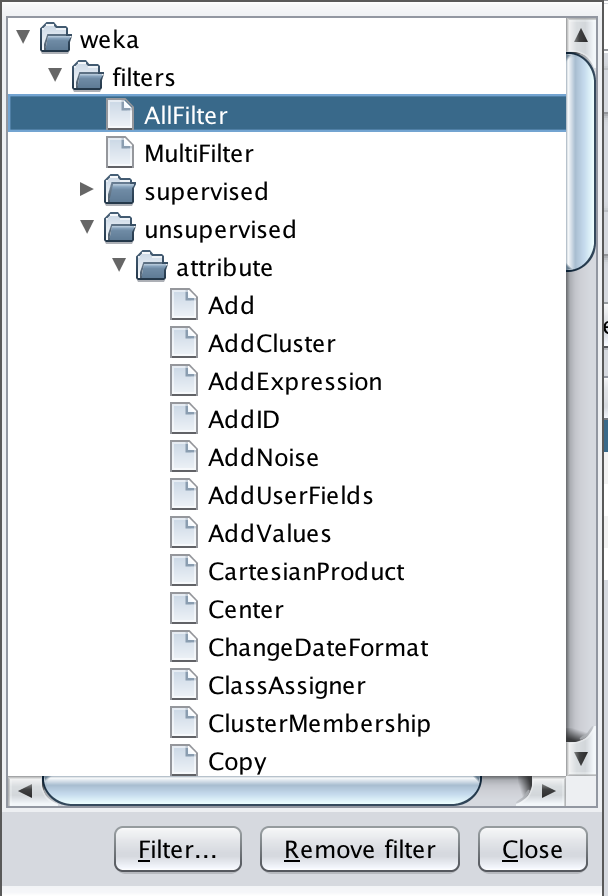
\includegraphics[width=0.45\textwidth]{images/B2_9a.png}}

\subfloat[An object editor.]{\label{subfig:filters_2}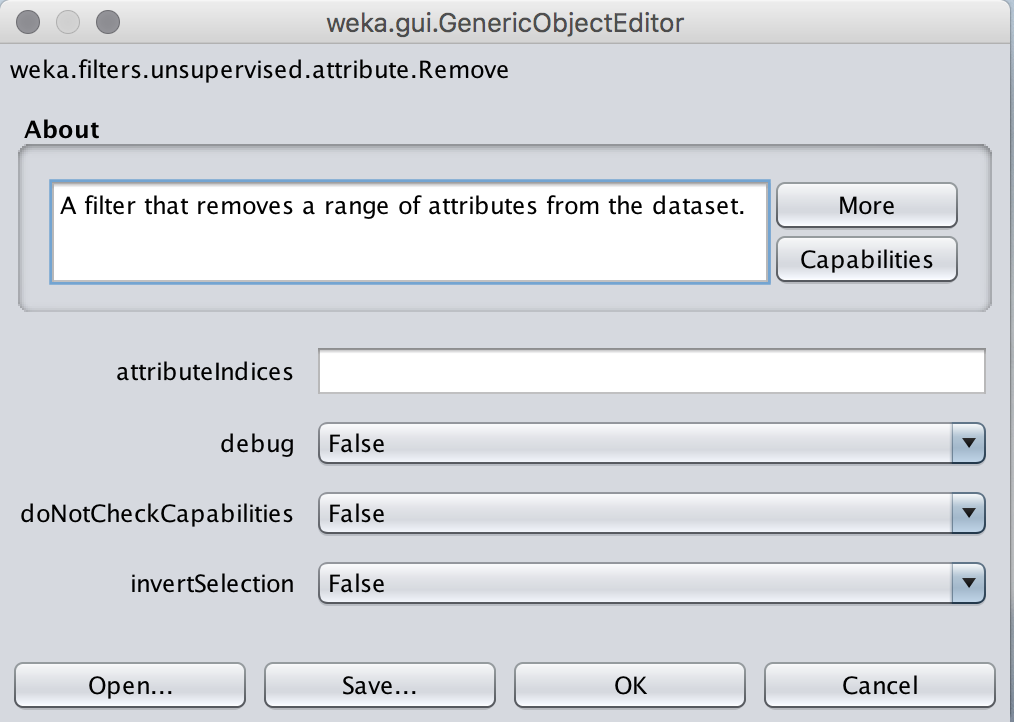
\includegraphics[width=0.45\textwidth]{images/B2_9b.png}}
\qquad
\subfloat[More information (click \textit{More}).]{\label{subfig:filters_3}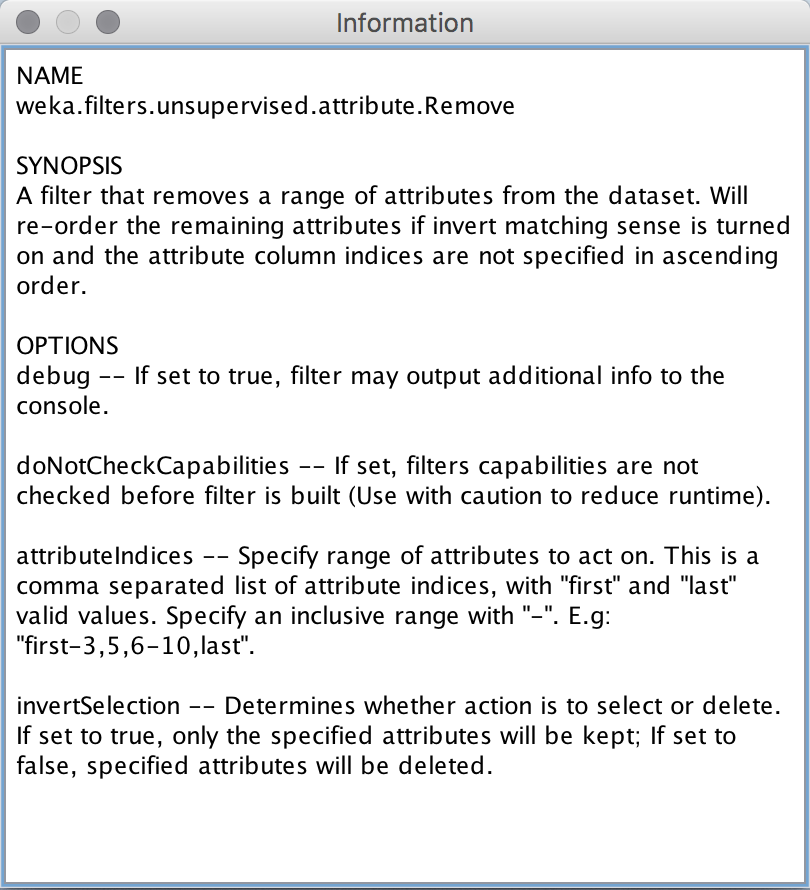
\includegraphics[width=0.45\textwidth]{images/B2_9c.png}}
\qquad
\subfloat[Information about the filter's capabilities (click \textit{Capabilities}).]{\label{subfig:filters_4}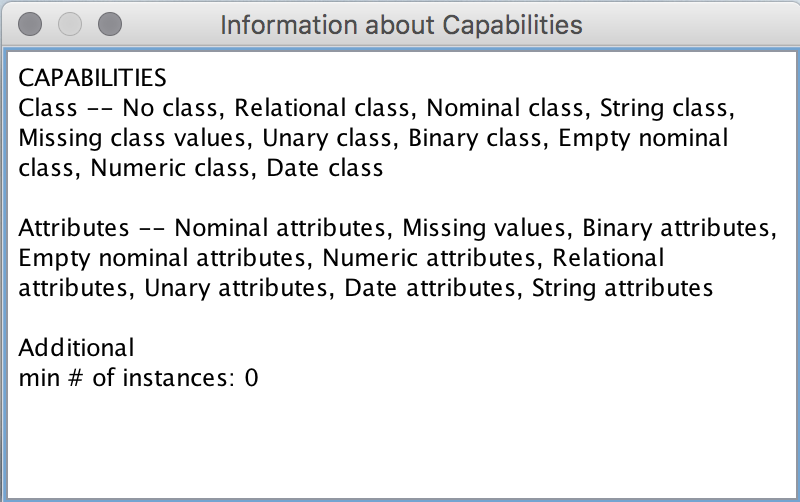
\includegraphics[width=0.45\textwidth]{images/B2_9d.png}}
\qquad
\subfloat[Constraints on capabilities.]{\label{subfig:filters_5}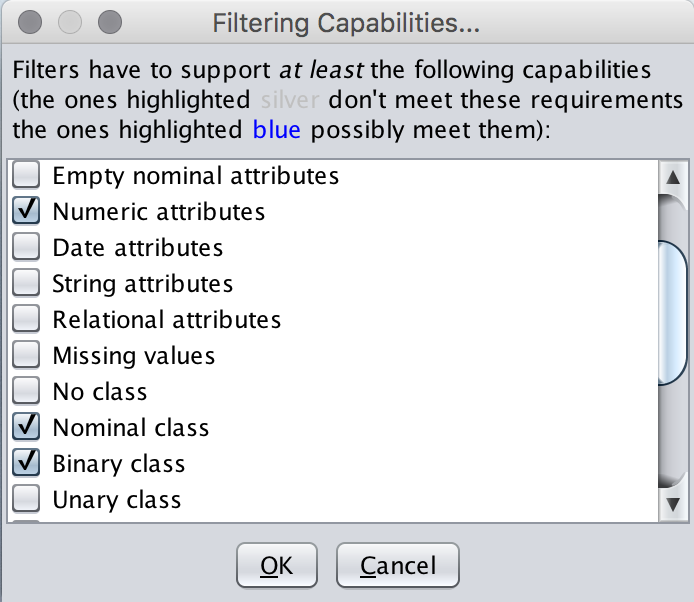
\includegraphics[width=0.45\textwidth]{images/B2_9e.png}}
\caption{\label{fig:filters}Choosing a filter.}
\end{figure}

Clicking \textit{Choose} (near the top left) in
Figure~\ref{subfig:explorer_2} gives a list of filters like that in
Figure~\ref{subfig:filters_1}. Actually, you get a collapsed version:
click on an arrow to open up its contents. We will describe how to use
a simple filter to delete specified attributes from a dataset, in
other words, to perform manual attribute selection. The same effect
can be achieved more easily by selecting the relevant attributes using
the tick boxes and pressing the \textit{Remove} button. Nevertheless
we describe the equivalent filtering operation explicitly, as an
example.

\textit{Remove} is an unsupervised attribute filter, and to see it you
must scroll further down the list. When selected, it appears in the
line beside the \textit{Choose} button, along with its parameter
values---in this case the line reads simply ``Remove''. Click that line
to bring up a generic object editor with which you can examine and
alter the filter's properties. (You did the same thing earlier by
clicking the \textit{J48} line in Figure~\ref{subfig:j48_2} to open
the \textit{J4.8} classifier's object editor.) The object editor for
the Remove filter shown in Figure~\ref{subfig:filters_2}.

To learn about it, click \textit{More} to show the information in
Figure~\ref{subfig:filters_3}. This explains that the filter removes a
range of attributes from the dataset. It has an option,
\textit{attributeIndices}, that specifies the range to act on and
another called \textit{invertSelection} that determines whether the
filter selects attributes or deletes them. There are boxes for both of
these in the object editor shown in Figure~\ref{subfig:filters_2}, and
in fact we have already set them to \textit{1,2} (to affect attributes
1 and 2, namely \textit{outlook} and \textit{temperature}) and
\textit{False} (to remove rather than retain them). Click \textit{OK}
to set these properties and close the box. Notice that the line beside
the \textit{Choose} button now reads \textit{Remove --R 1,2}. In the
command-line version of the \textit{Remove} filter, the option
\textit{--R} is used to specify which attributes to remove. After
configuring an object it's often worth glancing at the resulting
command-line formulation that the Explorer sets up.

Figure~\ref{fig:filters} demonstrates a further feature of the generic
object editor, namely ``capabilities.'' Algorithms in WEKA may provide
information about what data characteristics they can handle, and, if
they do, a \textit{Capabilities} button appears underneath
\textit{More} in the generic object editor
(Figure~\ref{subfig:filters_2}). Clicking it brings up
Figure~\ref{subfig:filters_4}, which gives information about what the
method can do. Here it states that \textit{Remove} can handle many
attribute characteristics, such as different types (nominal, numeric,
relational, etc.) and missing values. It shows the minimum number of
instances that are required for \textit{Remove} to operate on.

Figure~\ref{subfig:filters_5} shows a list of selected constraints on
capabilities, which is obtained by clicking the \textit{Filter} button
at the bottom of Figure~\ref{subfig:filters_1}. If the current dataset
exhibits some characteristic that is ticked in
Figure~\ref{subfig:filters_5} but missing from the capabilities for
the \textit{Remove} filter (Figure~\ref{subfig:filters_4}), the
\textit{Apply} button to the right of \textit{Choose} in
Figure~\ref{subfig:explorer_2} will be grayed out, as will the entry
in the list in Figure~\ref{subfig:filters_1}. Although you cannot
apply it, you can nevertheless select a grayed-out entry to inspect
its options, documentation and capabilities using the generic object
editor. You can release individual constraints by deselecting them in
Figure~\ref{subfig:filters_5}, or click the \textit{Remove filter}
button to clear all the constraints.

\begin{figure}[!ht]
\centering
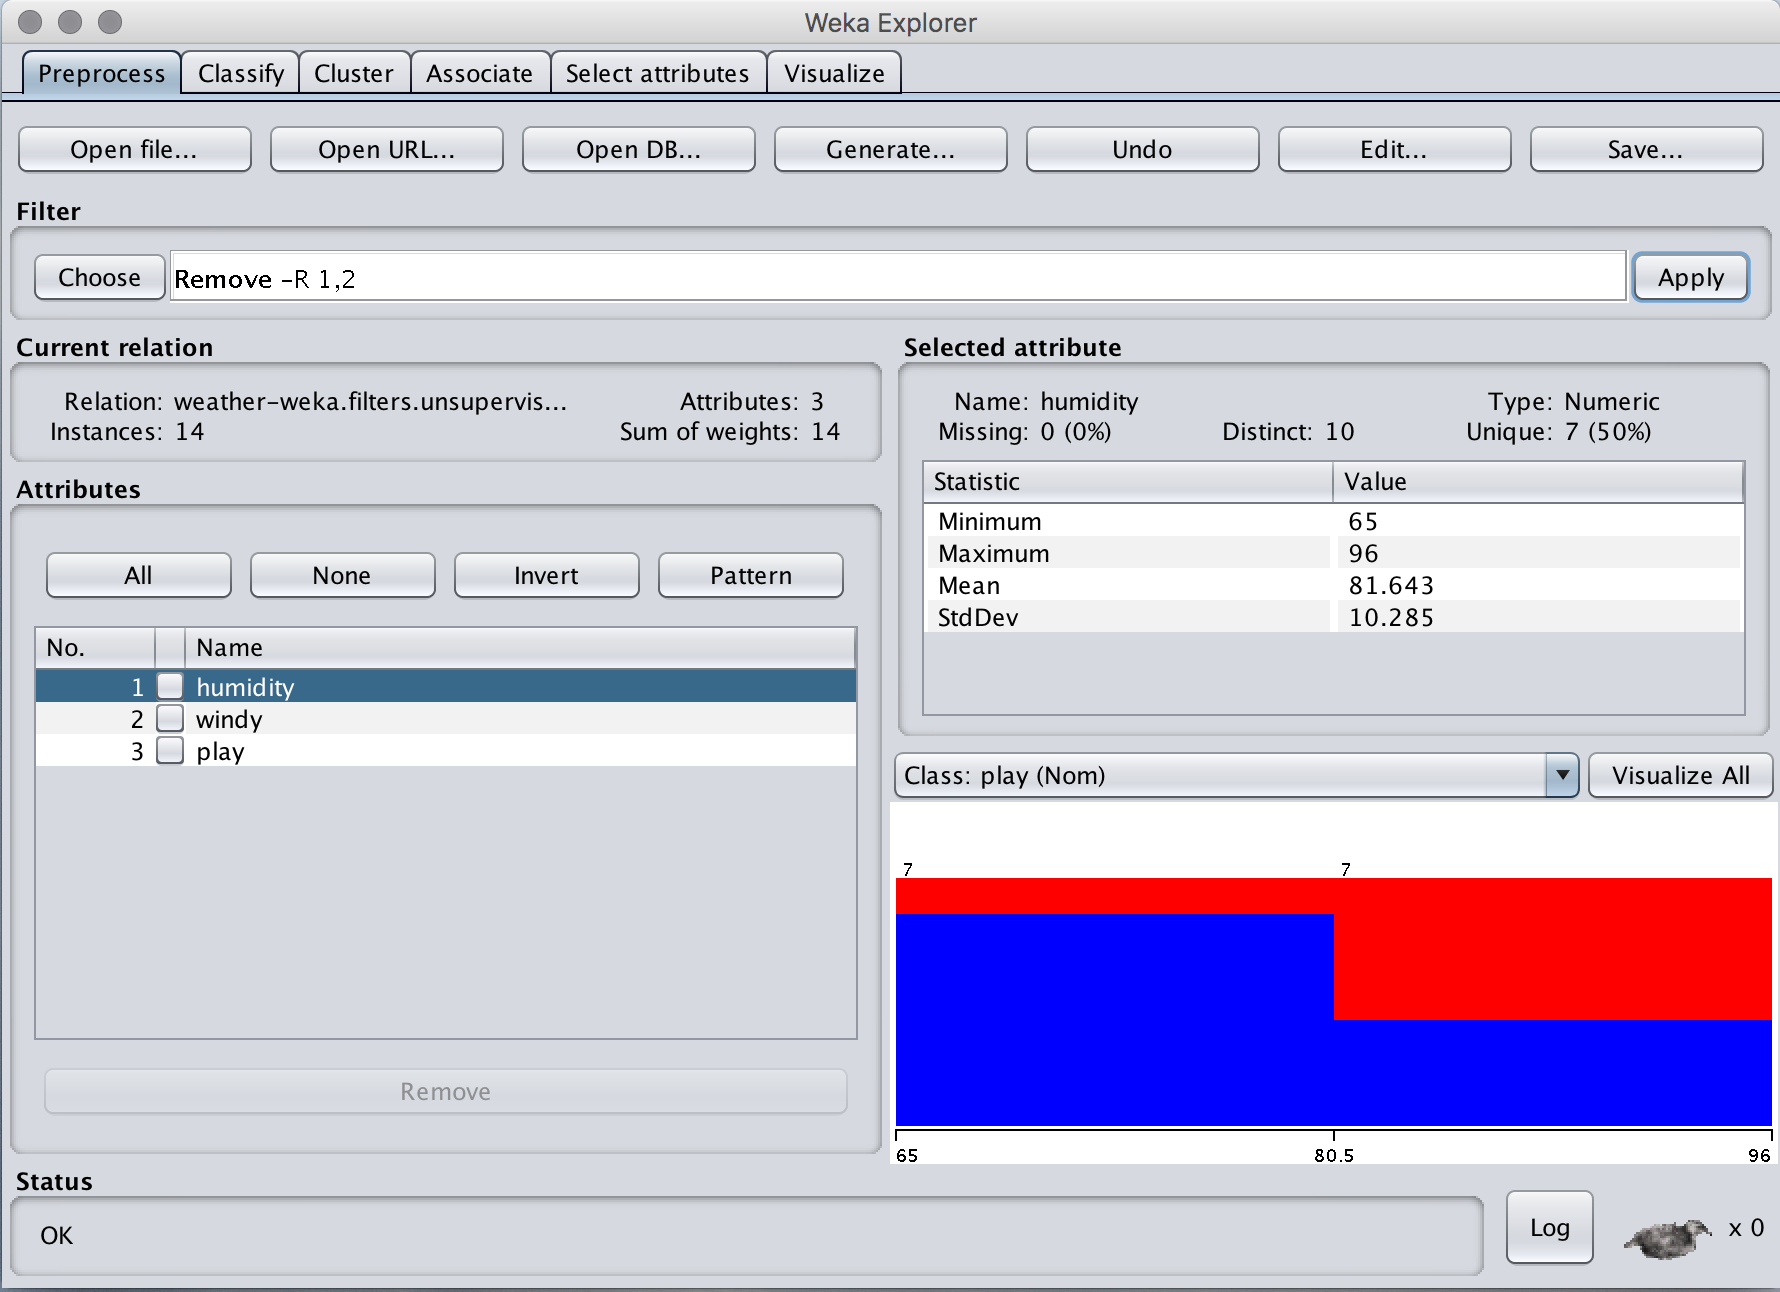
\includegraphics[width=0.9\textwidth]{images/B2_10.png}
\caption{The weather data with two attributes removed.}
\label{fig:weather_minus_two}
\end{figure}


Apply the filter by clicking \textit{Apply} (at the right-hand side of
Figure~\ref{subfig:explorer_2}). Immediately the screen in
Figure~\ref{fig:weather_minus_two} appears---just like the one in
Figure~\ref{subfig:explorer_2} but with only three attributes,
\textit{humidity}, \textit{windy}, and \textit{play}. At this point
the fifth button in the row near the top becomes active. \textit{Undo}
reverses the filtering operation and restores the original dataset,
which is useful when you experiment with different filters.

The first attribute, \textit{humidity}, is selected and a summary of
its values appears on the right. As a numeric attribute, the minimum
and maximum values, mean, and standard deviation are shown. Below is a
histogram that shows the distribution of the \textit{play}
attribute. Unfortunately, this display is impoverished because the
attribute has so few different values that they fall into two
equal-sized bins. More realistic datasets yield more informative
histograms.

\subsection{Training and testing learning schemes}

The \textit{Classify} panel lets you train and test learning schemes
that perform classification or
regression. Section~\ref{sect:getting_started} explained how to
interpret the output of a decision tree learner and showed the
performance figures that are automatically generated by the evaluation
module. The interpretation of these is the same for all models that
predict a categorical class. However, when evaluating models for
numeric prediction, WEKA produces a different set of performance
measures

\begin{figure}[!ht]
\centering
\subfloat[CPU data in the \textit{Preprocess} panel.]{\label{subfig:cpu_1}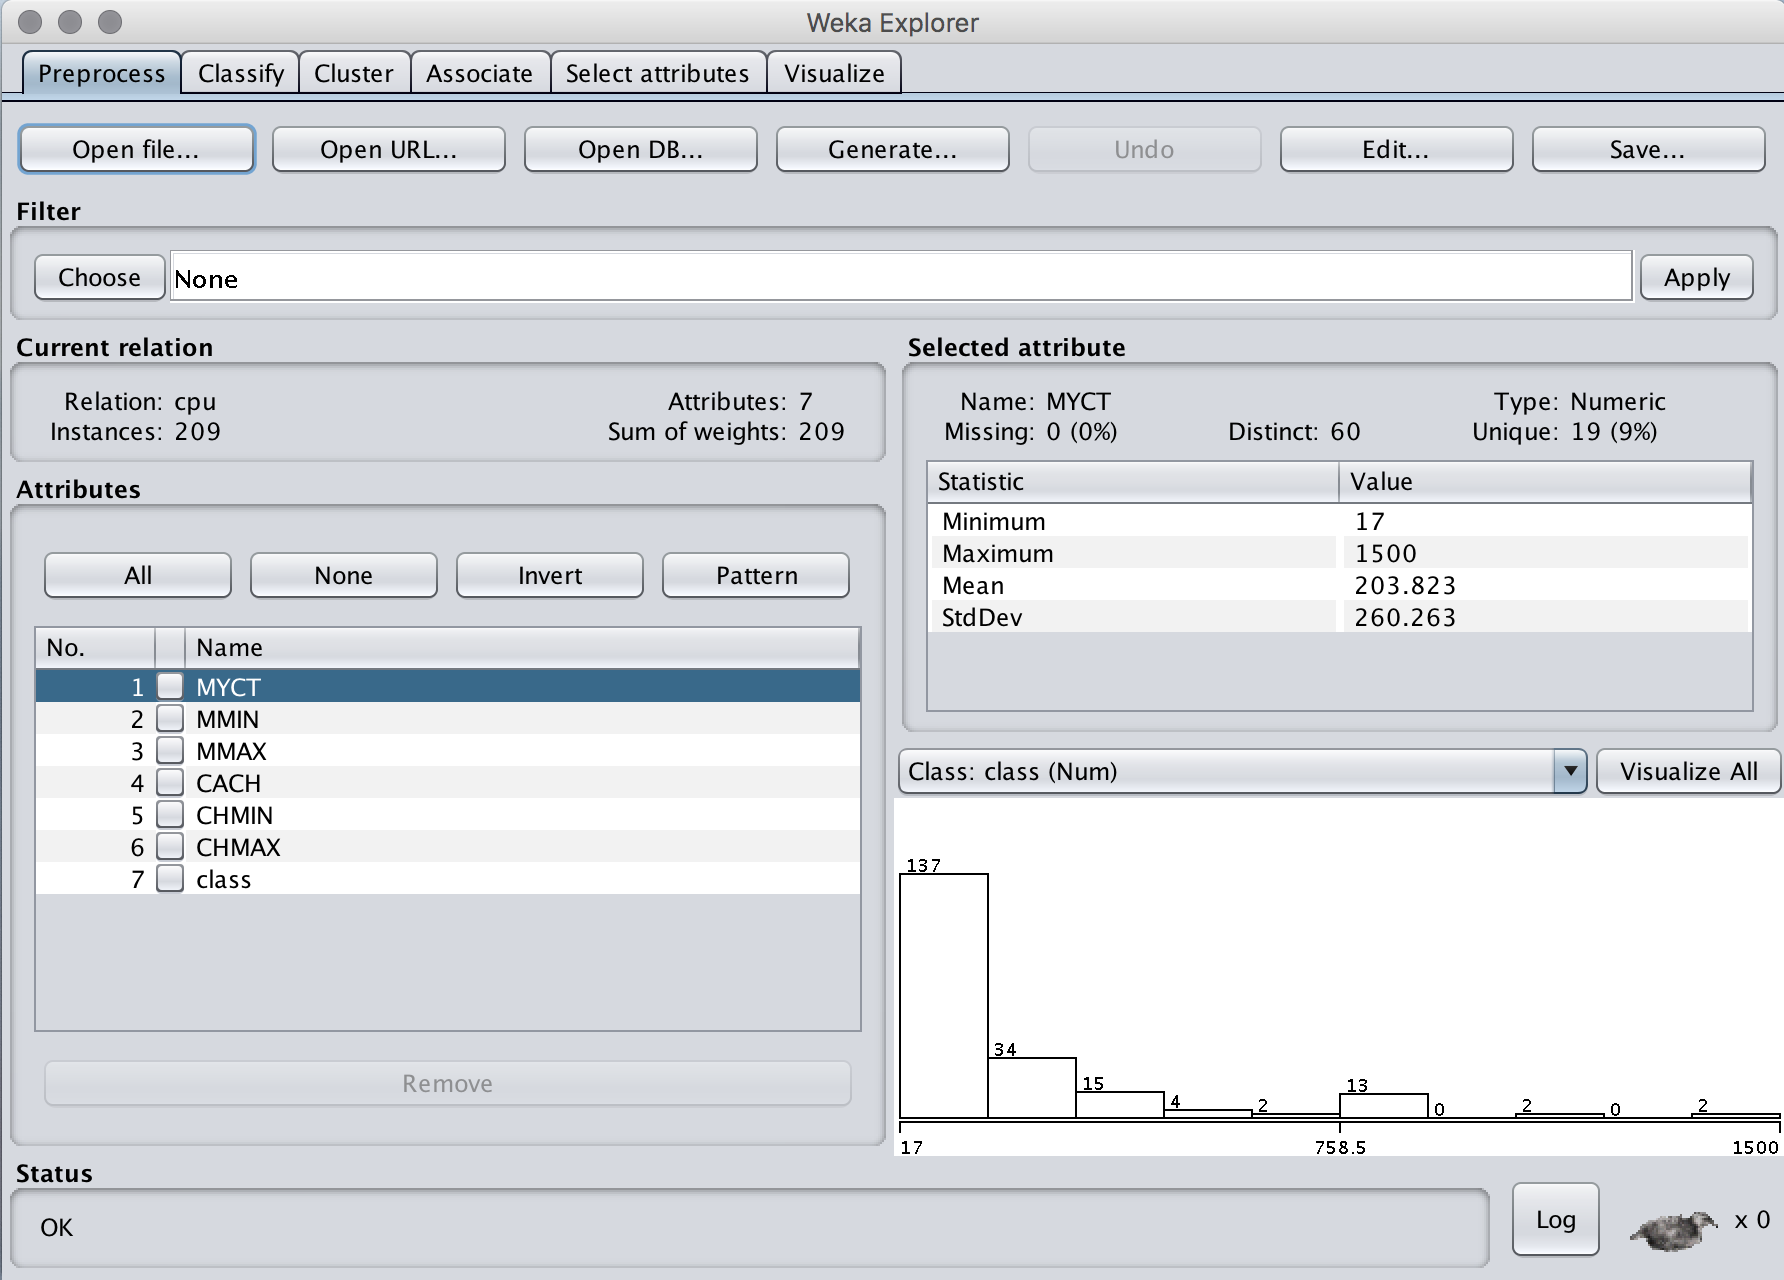
\includegraphics[width=0.9\textwidth]{images/B2_11a.png}}
\newline
\subfloat[\textit{M5'}'s performance on the CPU data.]{\label{subfig:cpu_2}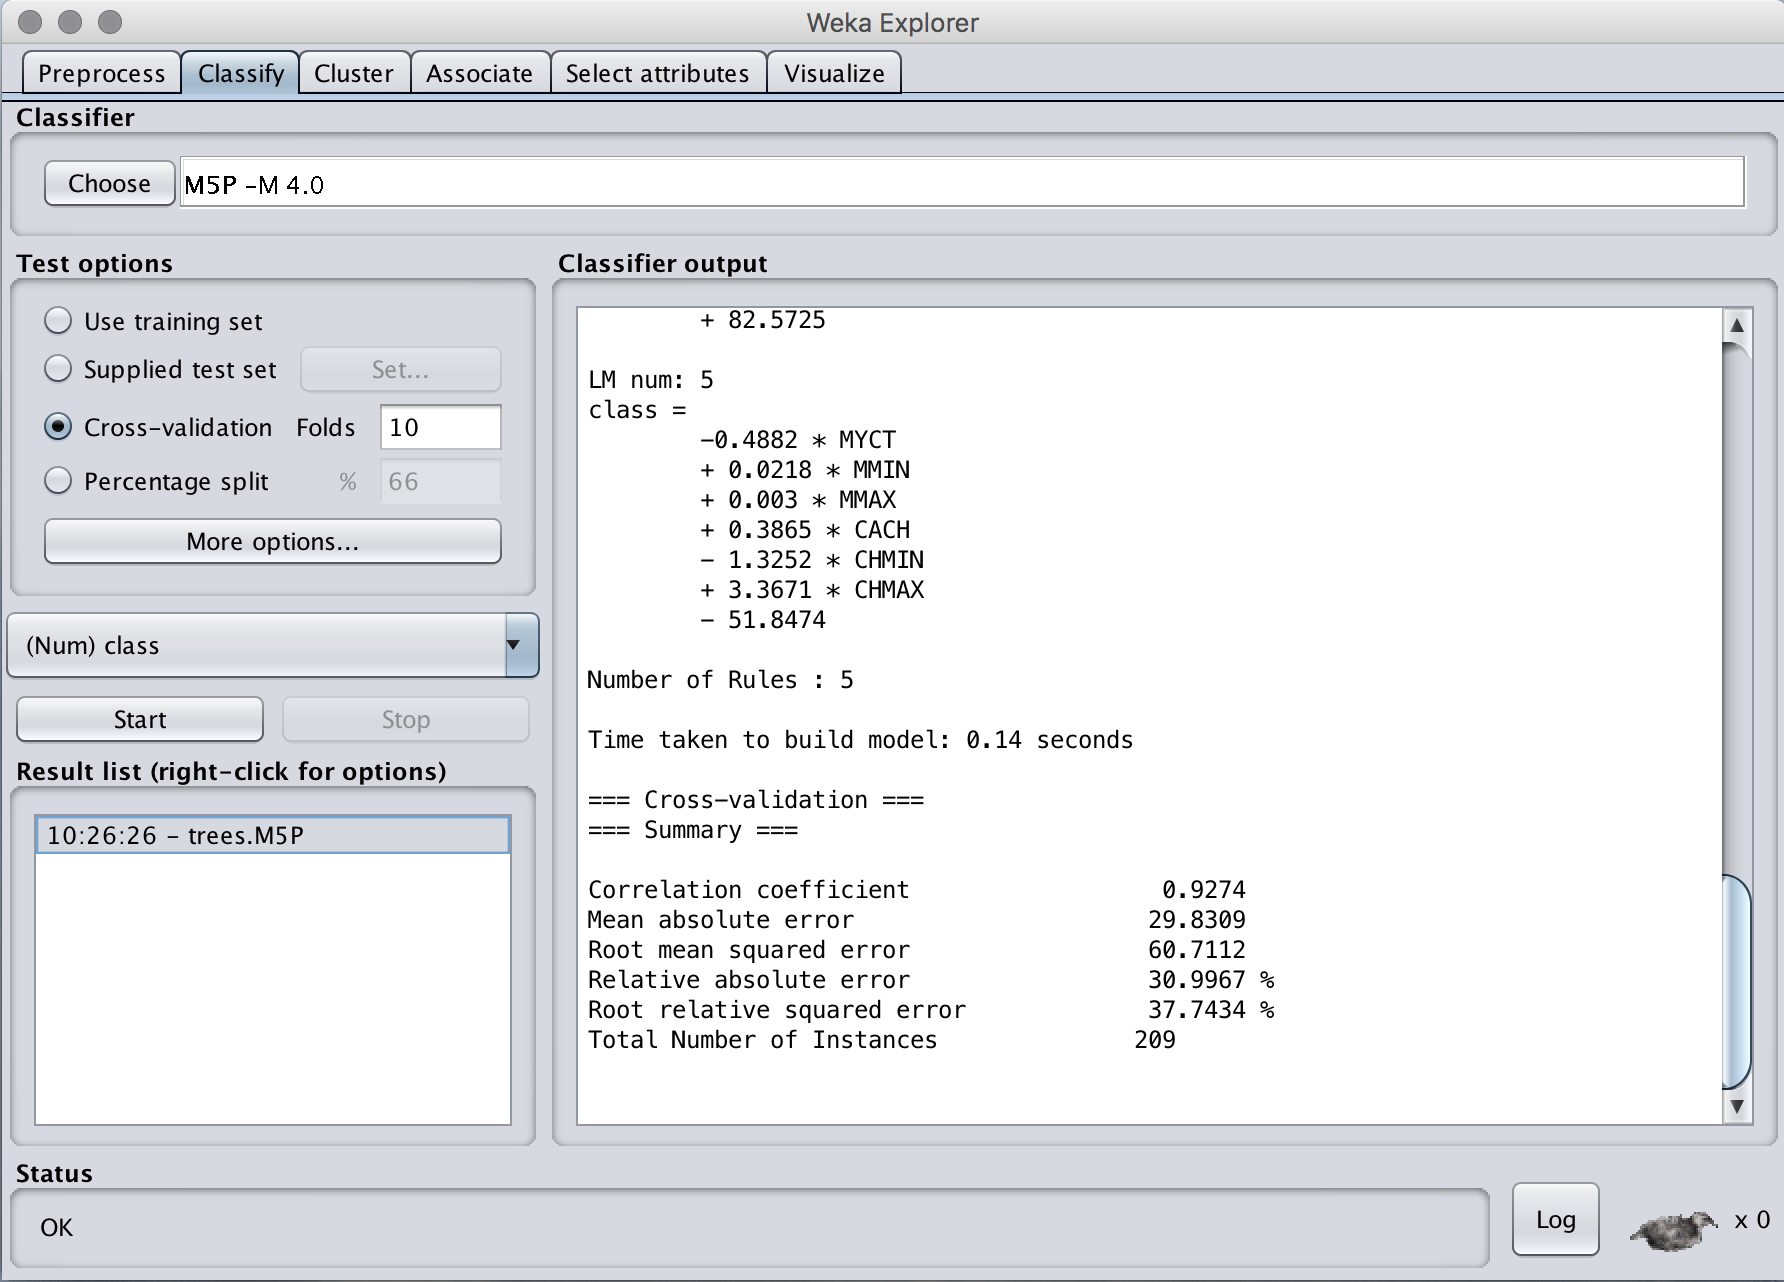
\includegraphics[width=0.9\textwidth]{images/B2_11b.png}}
\caption{\label{fig:cpu_m5}Processing the CPU performance data with \textit{M5'}.}
\end{figure}

As an example, in Figure~\ref{subfig:cpu_1} the CPU performance
dataset has been loaded into WEKA. You can see the histogram of values
of the first attribute, \textit{MYCT}, at the lower right. In
Figure~\ref{subfig:cpu_2} the model tree inducer M5' has been chosen
as the classifier by going to the \textit{Classify} panel, clicking
the \textit{Choose} button at the top left, opening up the trees
section of the hierarchical menu shown in Figure 2.4a, finding
\textit{M5P}, and clicking \textit{Start}. The hierarchy helps to
locate particular classifiers by grouping items with common
functionality

\begin{figure}[!p]
%\centering
\begin{mdframed}[innermargin=-1cm]
\begin{Verbatim}[fontsize=\footnotesize]
=== Run information ===

Scheme:       weka.classifiers.trees.M5P -M 4.0
Relation:     cpu
Instances:    209
Attributes:   7
              MYCT
              MMIN
              MMAX
              CACH
              CHMIN
              CHMAX
              class
Test mode:    10-fold cross-validation

=== Classifier model (full training set) ===

M5 pruned model tree:
(using smoothed linear models)

CHMIN <= 7.5 : LM1 (165/12.903%)
CHMIN >  7.5 : 
|   MMAX <= 28000 : 
|   |   MMAX <= 13240 : 
|   |   |   CACH <= 81.5 : LM2 (6/18.551%)
|   |   |   CACH >  81.5 : LM3 (4/30.824%)
|   |   MMAX >  13240 : LM4 (11/24.185%)
|   MMAX >  28000 : LM5 (23/48.302%)

LM num: 1
class = 
-0.0055 * MYCT + 0.0013 * MMIN + 0.0029 * MMAX + 0.8007 * CACH + 0.4015 * CHMAX 
  + 11.0971

LM num: 2
class = 
-1.0307 * MYCT + 0.0086 * MMIN + 0.0031 * MMAX + 0.7866 * CACH - 2.4503 * CHMIN 
  + 1.1597 * CHMAX + 70.8672

LM num: 3
class = -1.1057 * MYCT + 0.0086 * MMIN + 0.0031 * MMAX + 0.7995 * CACH 
  - 2.4503 * CHMIN + 1.1597 * CHMAX + 83.0016

LM num: 4
class = -0.8813 * MYCT + 0.0086 * MMIN + 0.0031 * MMAX + 0.6547 * CACH 
  - 2.3561 * CHMIN + 1.1597 * CHMAX + 82.5725

LM num: 5
class = -0.4882 * MYCT + 0.0218 * MMIN + 0.003 * MMAX + 0.3865 * CACH 
  - 1.3252 * CHMIN + 3.3671 * CHMAX - 51.8474

Number of Rules : 5

Time taken to build model: 0.14 seconds

=== Cross-validation ===
=== Summary ===

Correlation coefficient                  0.9274
Mean absolute error                     29.8309
Root mean squared error                 60.7112
Relative absolute error                 30.9967 %
Root relative squared error             37.7434 %
Total Number of Instances              209
\end{Verbatim}
\end{mdframed}
\caption{\label{fig:m5p_output}Output from the M5' program for numeric prediction.}
\end{figure}

Figure~\ref{fig:m5p_output} shows the output. The pruned model tree
contains splits on three of the six attributes in the data. The root
splits on the \textit{CHMIN} attribute, yielding a linear model at the
leaf on the left-hand branch and the remaining structure in the
right-hand branch. There are five leaves in all, each with a
corresponding linear model. The first number in parentheses at each
leaf is the number of instances that reach it; the second is the root
mean squared error of the predictions from the leaf's linear model for
those instances, expressed as a percentage of the standard deviation
of the class attribute computed over all the training data. The
description of the tree is followed by several figures that measure
its performance. These are derived from the test option chosen in
Figure 2.11b, 10-fold cross-validation (not stratified, because
stratification does not apply when the class is numeric).

Ordinary linear regression, another scheme for numeric prediction, is
found under \textit{LinearRegression} in the {\em functions} section of the
menu in Figure~\ref{subfig:j48_1}. It builds a single linear
regression model rather than the five in Figure~\ref{fig:m5p_output};
not surprisingly, its performance is slightly worse.

\begin{figure}[!ht]
\centering
\subfloat[M5'.]{\label{subfig:regression_errors_1}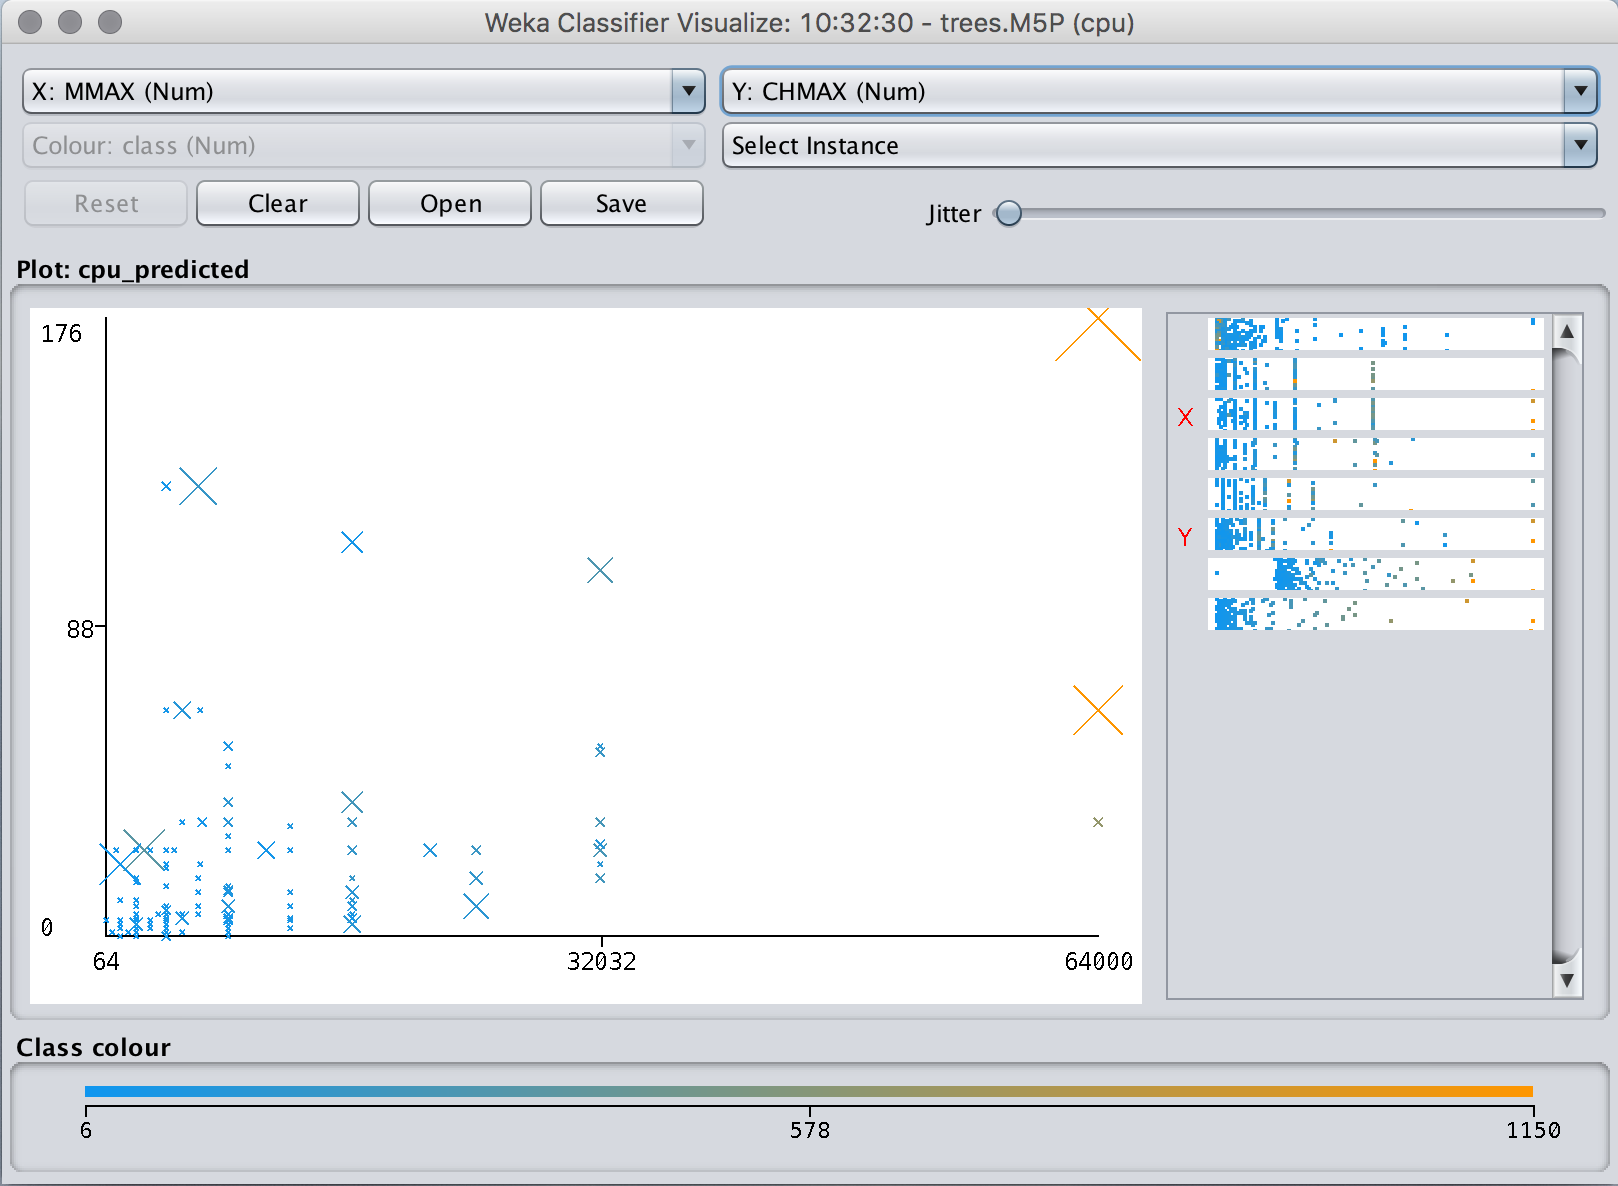
\includegraphics[width=0.9\textwidth]{images/B2_13a.png}}
\newline
\subfloat[Linear regression.]{\label{subfig:regression_errors_2}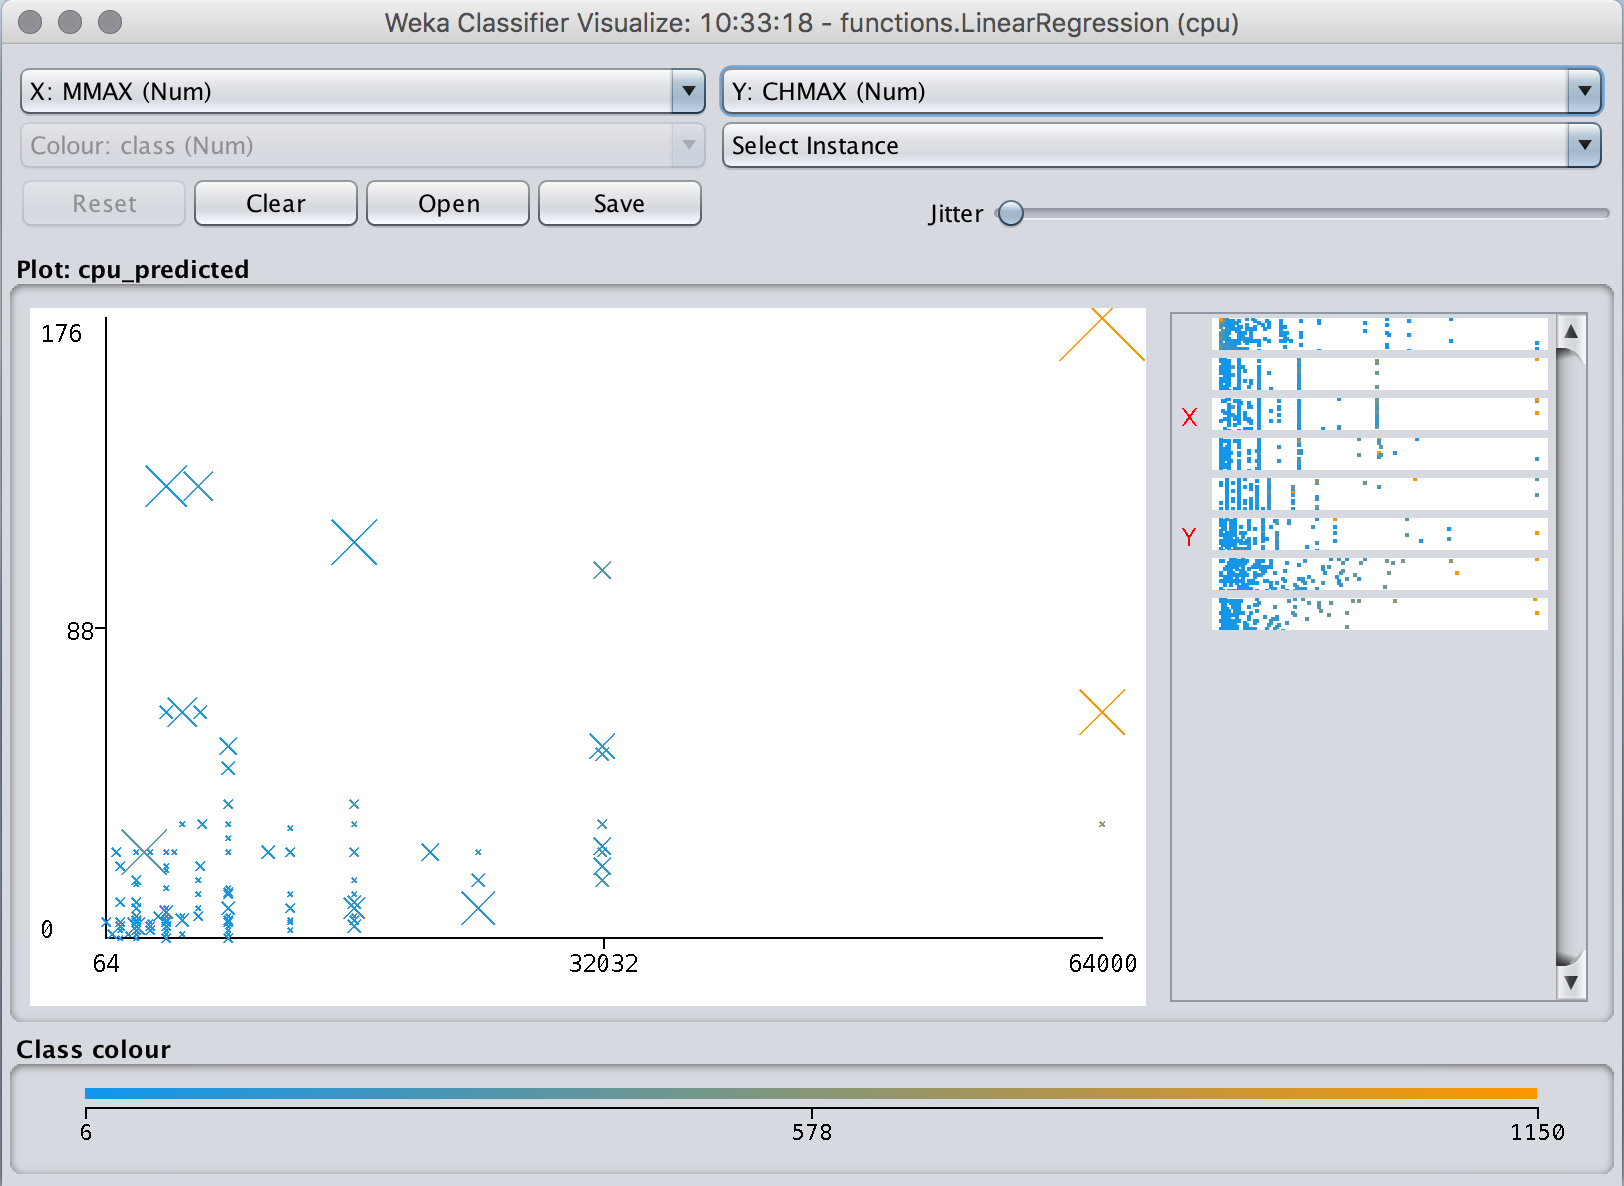
\includegraphics[width=0.9\textwidth]{images/B2_13b.png}}
\caption{\label{fig:regression_errors}Visualizing errors.}
\end{figure}


To get a feel for their relative performance, let us visualize the
errors these schemes make, as we did for the iris dataset in
Figure~\ref{subfig:j48_4}. Right-click the entry in the history list
and select \textit{Visualize classifier errors} to bring up the
two-dimensional plot of the data in
Figure~\ref{fig:regression_errors}. The points are color coded by
class---but in this case the color varies continuously because the
class is numeric. In Figure~\ref{fig:regression_errors} the
\textit{MMAX} attribute has been selected for the X-axis and
\textit{CHMAX} has been chosen for the Y-axis because this gives a
reasonable spread of points. Each data point is marked by a cross
whose size indicates the absolute value of the error for that
instance. The smaller crosses in
Figure~\ref{subfig:regression_errors_1} (for M5'), when compared with
those in Figure~\ref{subfig:regression_errors_2} (for linear
regression), show that M5' is superior.

\subsection{Using a metalearner}

\begin{figure}[!ht]
\centering
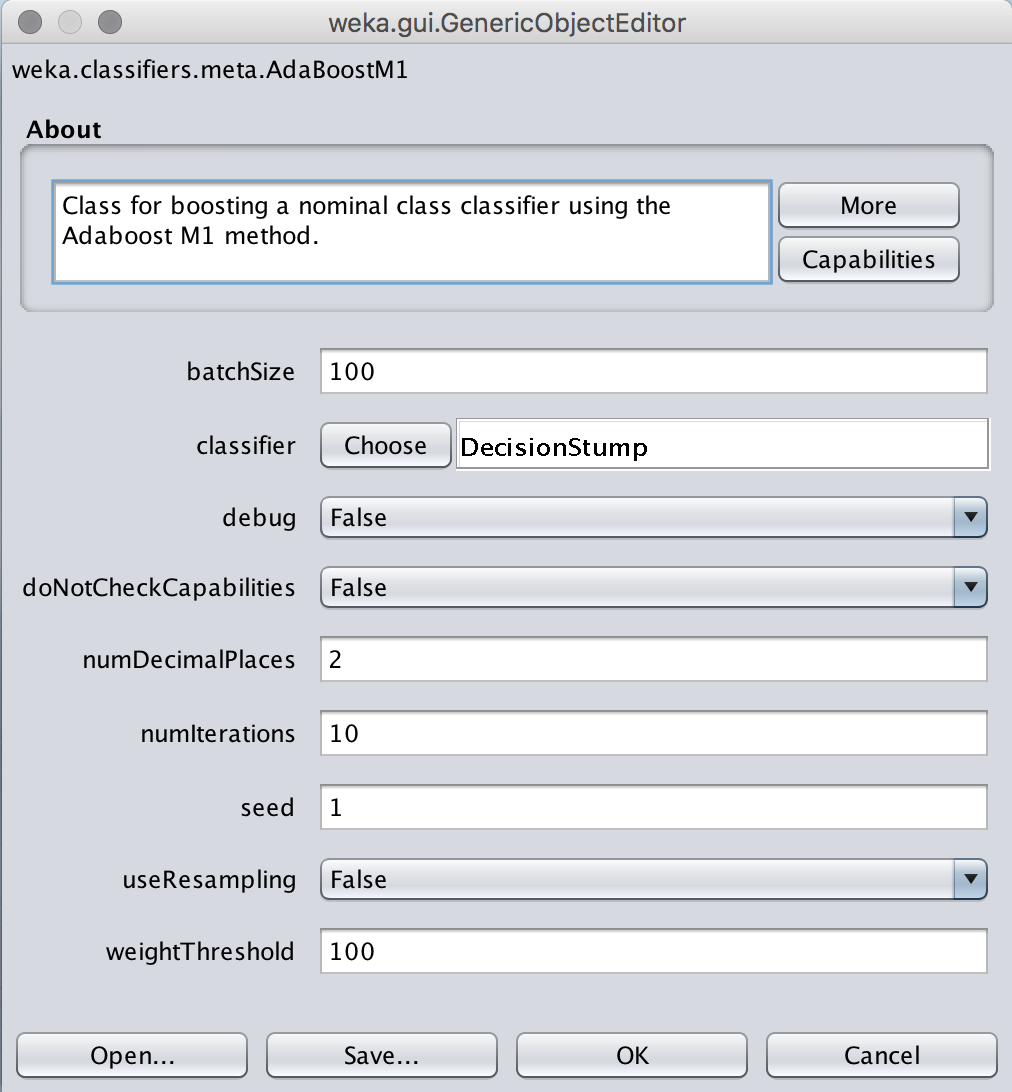
\includegraphics[width=0.7\textwidth]{images/B2_14.png}
\caption{Configuring a metalearner for boosting decision stumps.}
\label{fig:config_metalearner}
\end{figure}


Metalearners take simple classifiers and turn them into more powerful
learners. For example, to boost decision stumps in the Explorer, go to
the \textit{Classify} panel and choose the classifier
\textit{AdaboostM1} from the meta section of the hierarchical
menu. When you configure this classifier by clicking it, the object
editor shown in Figure~\ref{fig:config_metalearner} appears. This has
its own classifier field, which we set to \textit{DecisionStump} (as
shown). This method could itself be configured by clicking (except
that \textit{DecisionStump} happens to have no editable
properties). Click \textit{OK} to return to the main \textit{Classify}
panel and {\em Start} to try out boosting decision stumps up to 10 times. It
turns out that this mislabels only 7 of the 150 instances in the iris
data---good performance considering the rudimentary nature of decision
stumps and the rather small number of boosting iterations.

\subsection{Clustering and association rules}

Use the \textit{Cluster} and \textit{Associate} panels to invoke
clustering algorithms and methods for finding association rules. When
clustering, WEKA shows the number of clusters and how many instances
each cluster contains. For some algorithms the number of clusters can
be specified by setting a parameter in the object editor. For
probabilistic clustering methods, WEKA measures the log-likelihood of
the clusters on the training data: the larger this quantity, the
better the model fits the data. Increasing the number of clusters
normally increases the likelihood, but may overfit.

The controls on the \textit{Cluster} panel are similar to those for
\textit{Classify}. You can specify some of the same evaluation
methods---use training set, supplied test set, and percentage split
(the last two are used with the log-likelihood). A further method,
classes to clusters evaluation, compares how well the chosen clusters
match a preassigned class in the data. You select an attribute (which
must be nominal) that represents the ``true'' class. Having clustered
the data, WEKA determines the majority class in each cluster and
prints a confusion matrix showing how many errors there would be if
the clusters were used instead of the true class. If your dataset has
a class attribute, you can ignore it during clustering by selecting it
from a pull-down list of attributes, and see how well the clusters
correspond to actual class values. Finally, you can choose whether or
not to store the clusters for visualization. The only reason not to do
so is to conserve space. As with classifiers, you visualize the
results by right-clicking on the result list, which allows you to view
two-dimensional scatter plots like the one in
Figure~\ref{subfig:j48_4}. If you have chosen classes to clusters
evaluation, the class assignment errors are shown. For the
\textit{Cobweb} clustering scheme, you can also visualize the tree.

\begin{figure}[!ht]
%\centering
\begin{mdframed}[innermargin=-1.5cm]
\begin{Verbatim}[fontsize=\scriptsize]
 1. outlook=overcast 4 ==> play=yes 4 <conf:(1)> lift:(1.56) lev:(0.1) [1] conv:(1.43)
 2. temperature=cool 4 ==> humidity=normal 4 <conf:(1)> lift:(2) lev:(0.14) [2] conv:(2)
 3. humidity=normal windy=FALSE 4 ==> play=yes 4 <conf:(1)> lift:(1.56) lev:(0.1) [1] conv:(1.43)
 4. outlook=sunny play=no 3 ==> humidity=high 3 <conf:(1)> lift:(2) lev:(0.11) [1] conv:(1.5)
 5. outlook=sunny humidity=high 3 ==> play=no 3 <conf:(1)> lift:(2.8) lev:(0.14) [1] conv:(1.93)
 6. outlook=rainy play=yes 3 ==> windy=FALSE 3 <conf:(1)> lift:(1.75) lev:(0.09) [1] conv:(1.29)
 7. outlook=rainy windy=FALSE 3 ==> play=yes 3 <conf:(1)> lift:(1.56) lev:(0.08) [1] conv:(1.07)
 8. temperature=cool play=yes 3 ==> humidity=normal 3 <conf:(1)> lift:(2) lev:(0.11) [1] conv:(1.5)
 9. outlook=sunny temperature=hot 2 ==> humidity=high 2 <conf:(1)> lift:(2) lev:(0.07) [1] conv:(1)
10. temperature=hot play=no 2 ==> outlook=sunny 2 <conf:(1)> lift:(2.8) lev:(0.09) [1] conv:(1.29)
\end{Verbatim}
\end{mdframed}
\caption{\label{fig:apriori_output}Output from the Apriori program for association rules.}
\end{figure}

The \textit{Associate} panel is simpler than \textit{Classify} or
\textit{Cluster}. WEKA contains several algorithms for determining
association rules and no methods for evaluating such
rules. Figure~\ref{fig:apriori_output} shows the output from the
Apriori program for association rules on the nominal version of the
weather data. Despite the simplicity of the data, several rules are
found. The number before the arrow is the number of instances for
which the antecedent is true; that after the arrow is the number of
instances for which the consequent is true also; and the confidence
(in parentheses) is the ratio between the two. Ten rules are found by
default: you can ask for more by using the object editor to change
\textit{numRules}.

\subsection{Attribute selection}

The \textit{Select attributes} panel gives access to several methods
for attribute selection. This involves an attribute evaluator and a
search method. Both are chosen in the usual way and configured with
the object editor. You must also decide which attribute to use as the
class. Attribute selection can be performed using the full training
set or using cross-validation. In the latter case it is done
separately for each fold, and the output shows how many times---that is,
in how many of the folds---each attribute was selected. The results are
stored in the history list. When you right-click an entry here you can
visualize the dataset in terms of the selected attributes (choose
\textit{Visualize reduced data}).

\subsection{Visualization}

\begin{figure}[!p]
\centering
\subfloat[Scatter plot matrix.]{\label{subfig:visualize_1}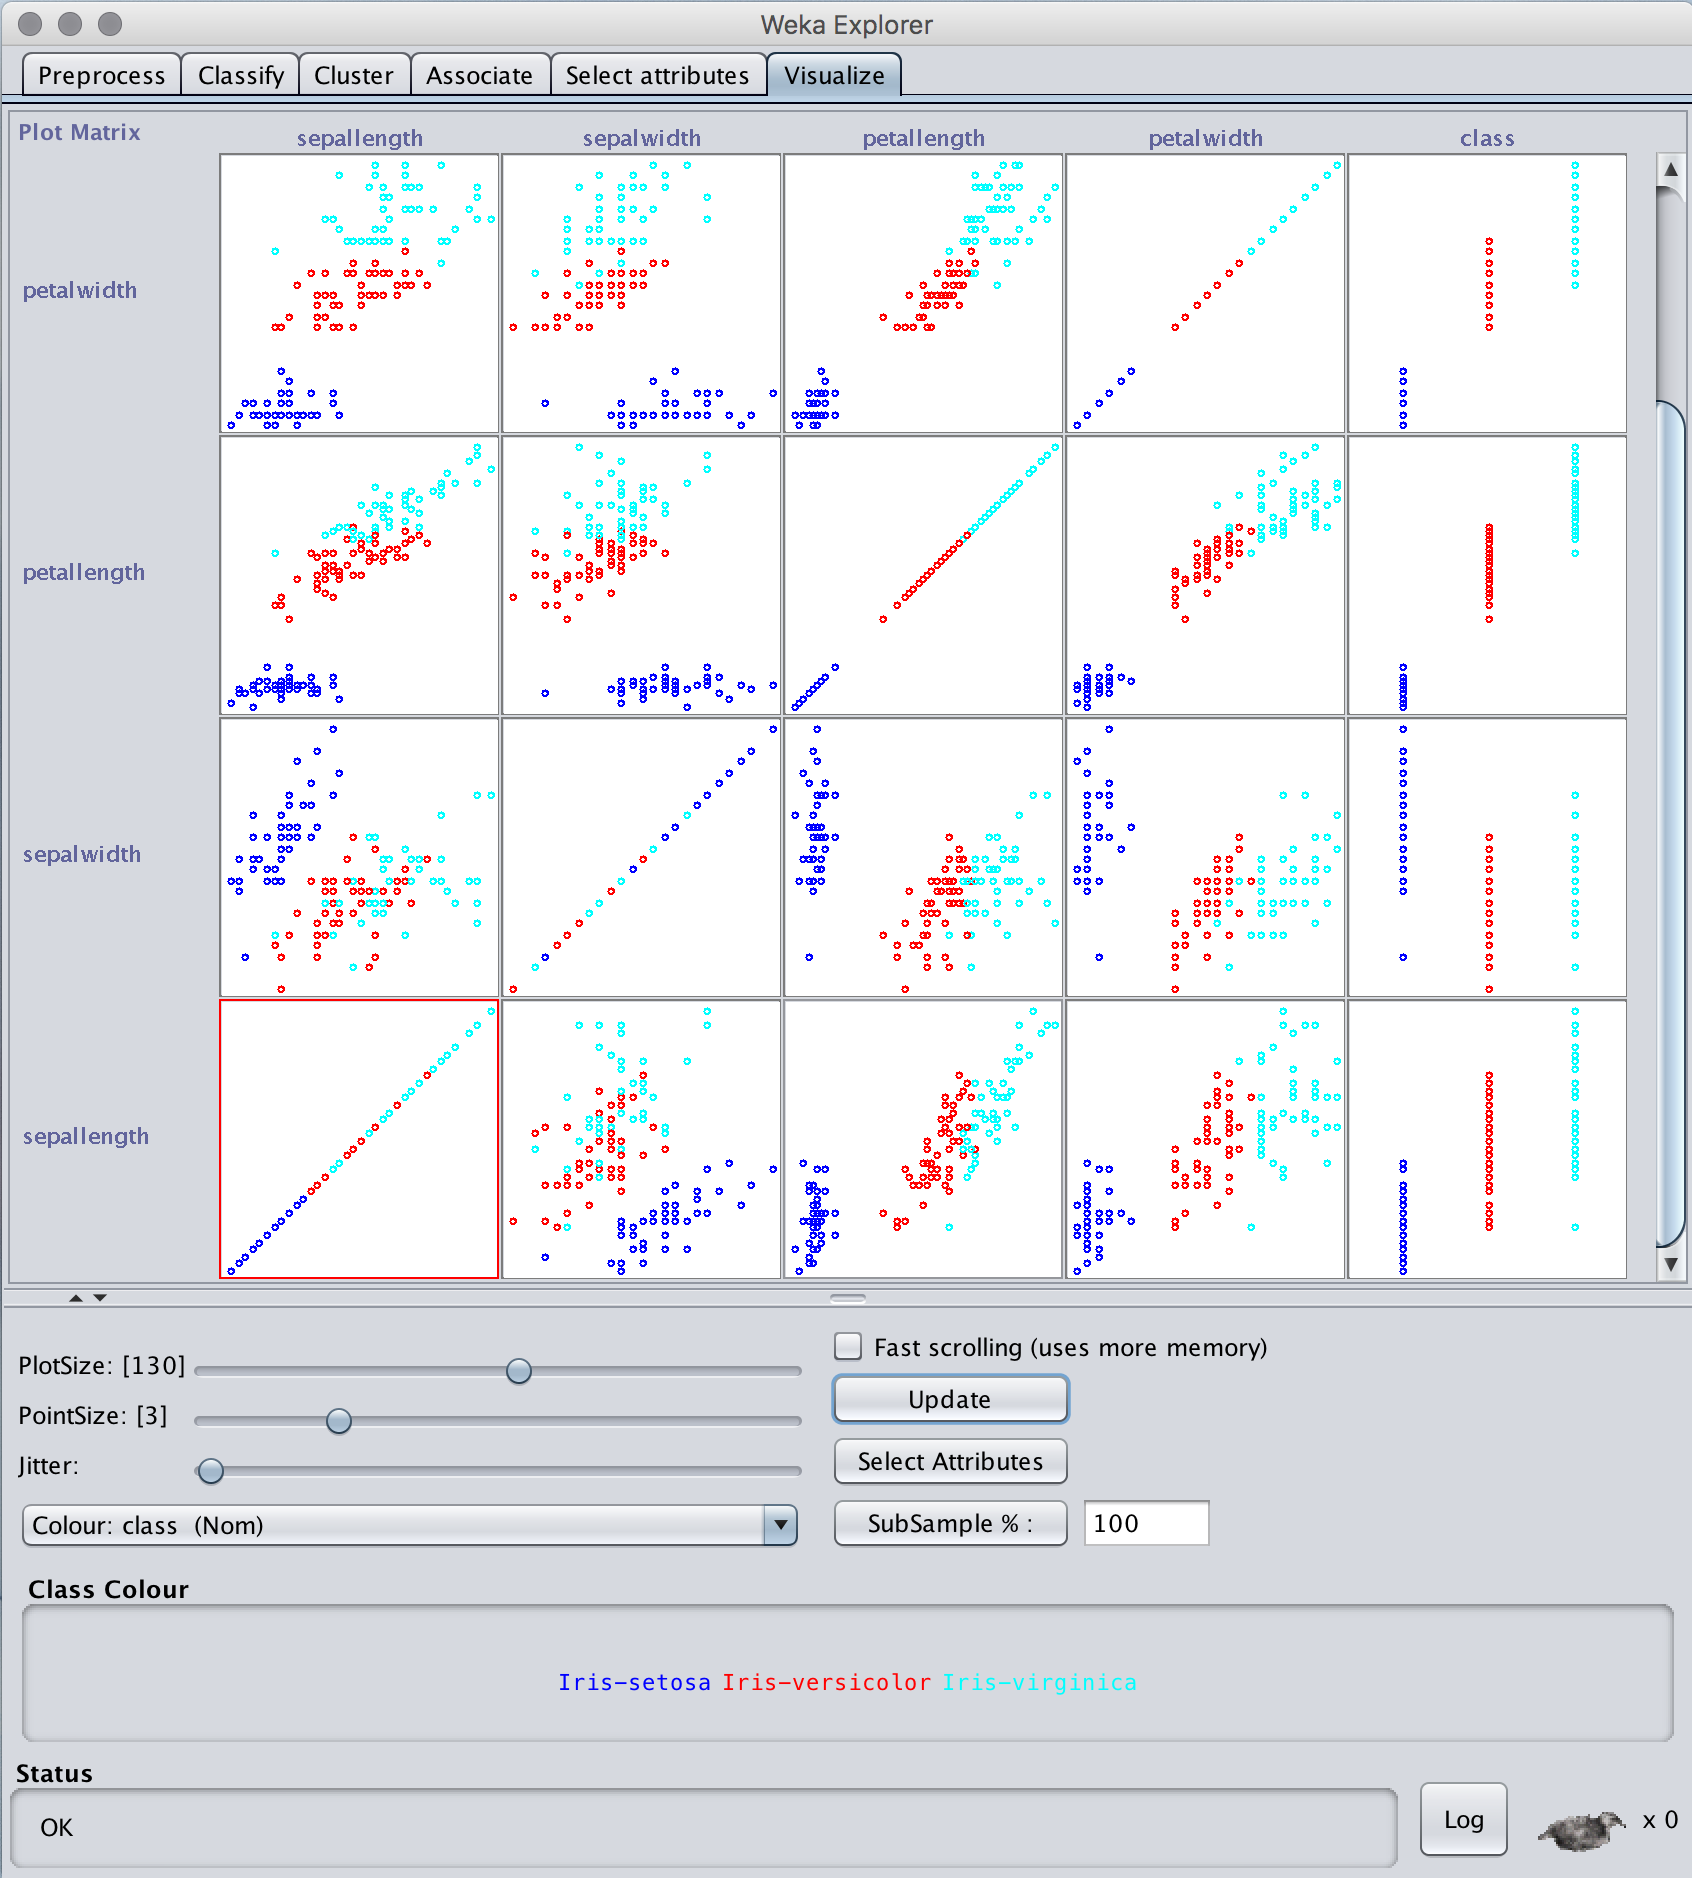
\includegraphics[width=0.8\textwidth]{images/B2_16a.png}}
\newline
\subfloat[Zoomed in on a cell from the matrix.]{\label{subfig:visualize_2}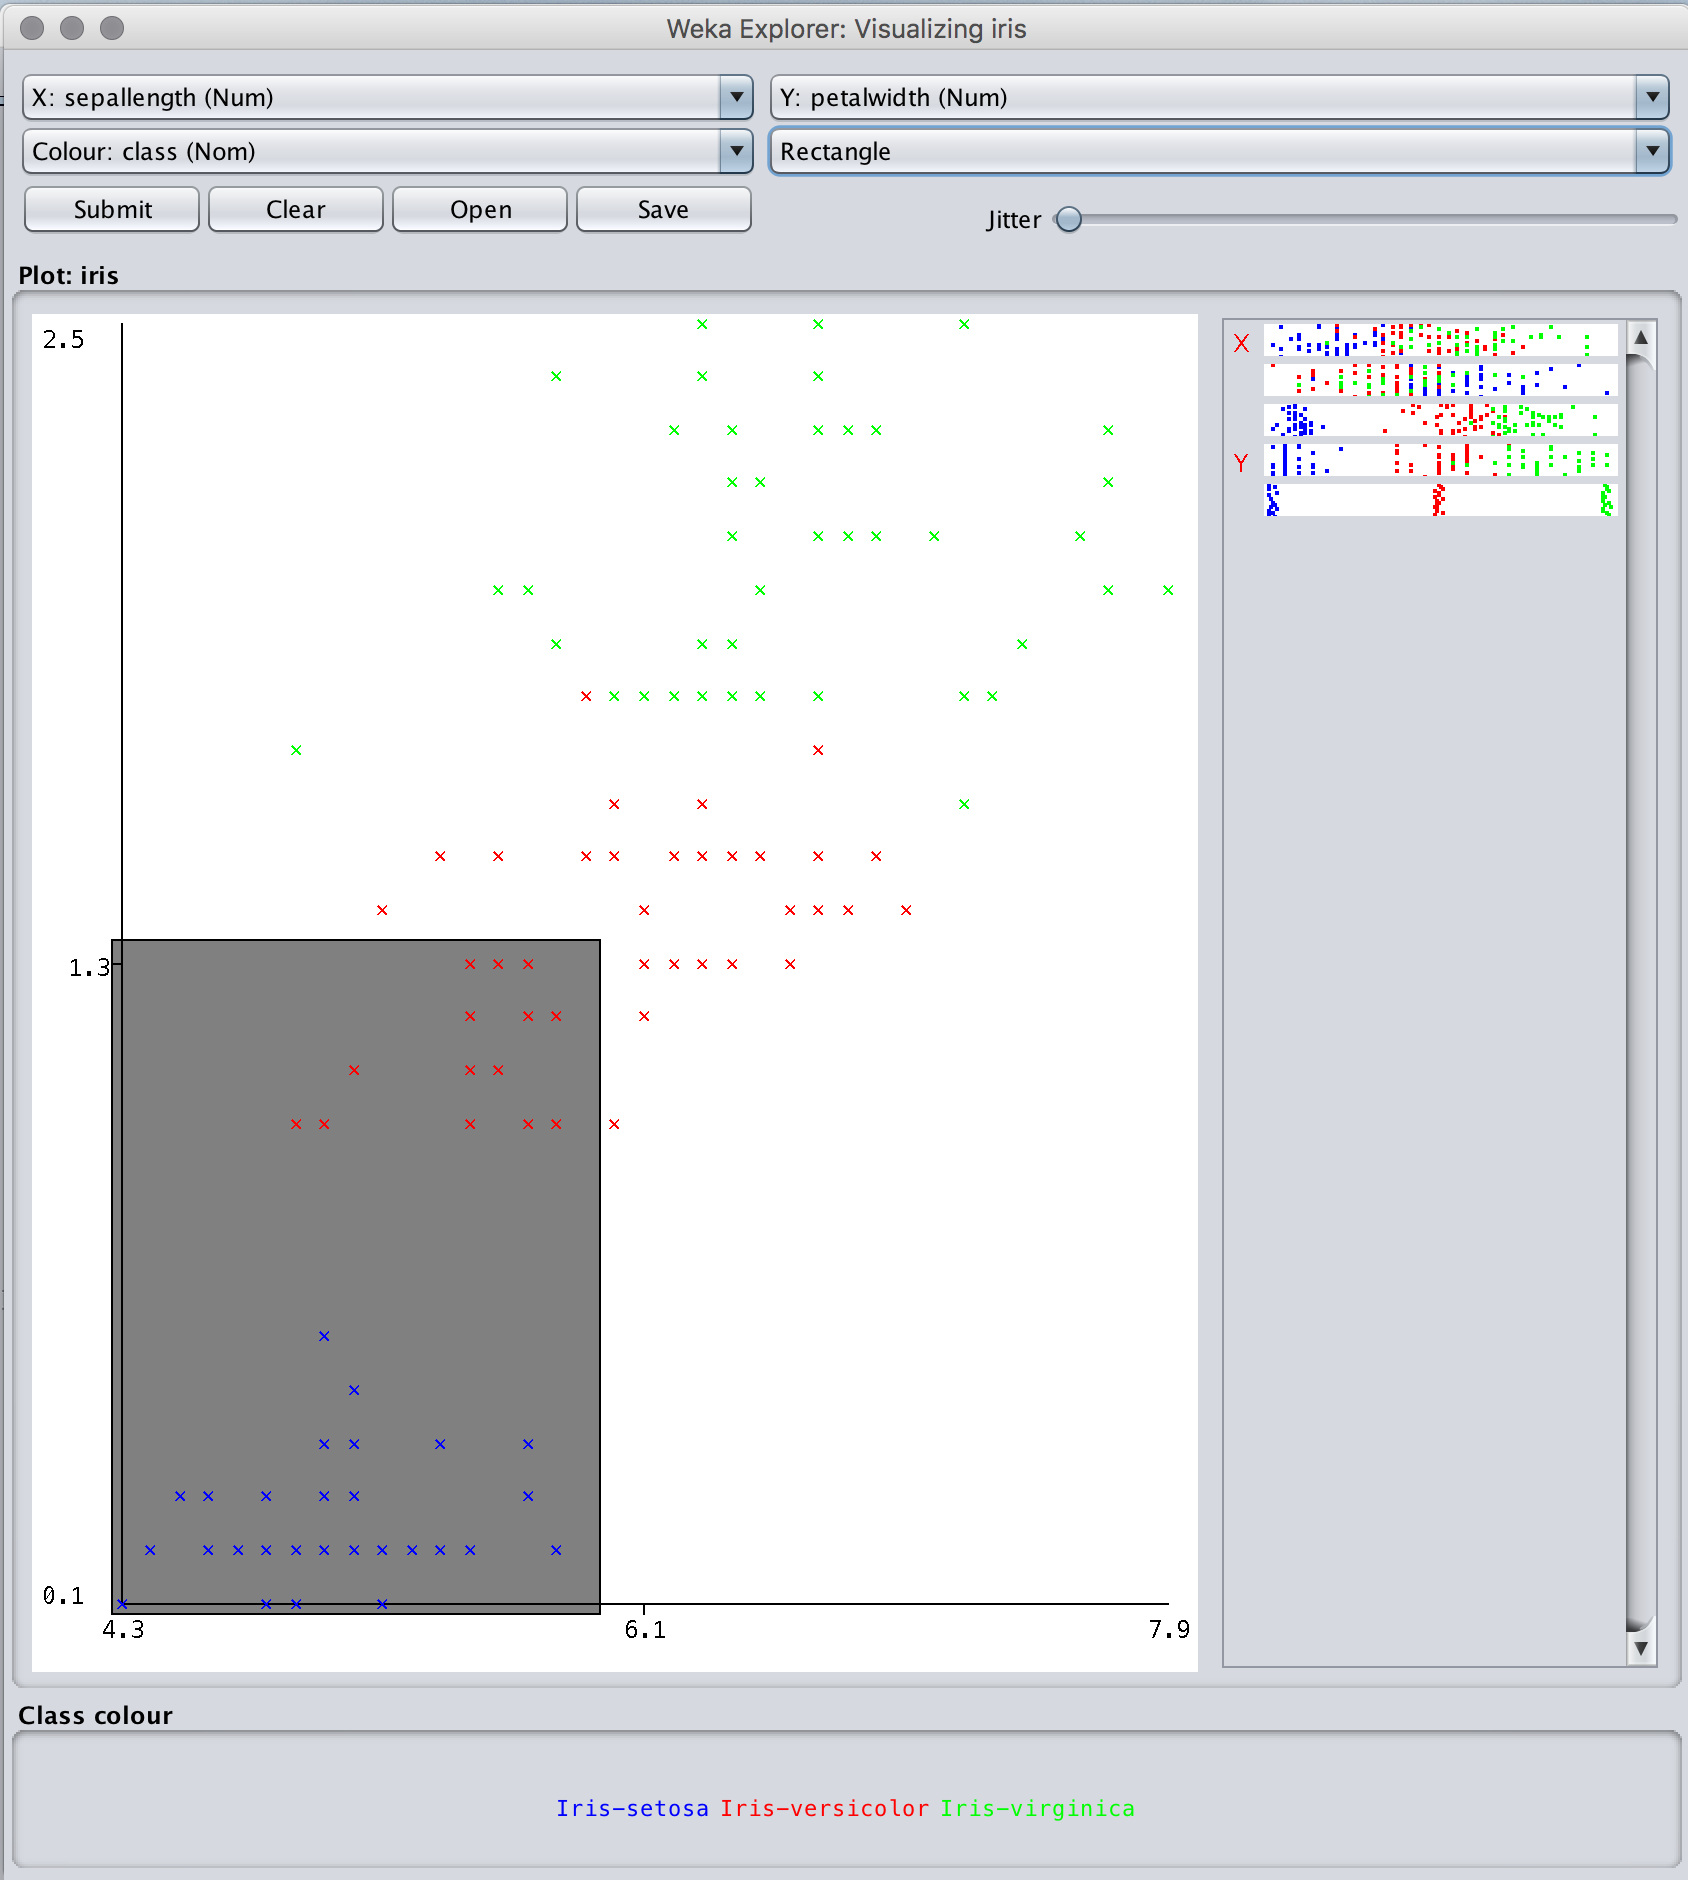
\includegraphics[width=0.8\textwidth]{images/B2_16b.png}}
\caption{\label{fig:regression_errors}Visualizing the iris data.}
\end{figure}


The \textit{Visualize} panel helps you visualize a dataset---not the
result of a classification or clustering model, but the dataset
itself. It displays a matrix of two-dimensional scatter plots of every
pair of attributes. Figure~\ref{subfig:visualize_1} shows the iris dataset. You can
select an attribute---normally the class---for coloring the data
points using the controls at the bottom. If it is nominal, the
coloring is discrete; if it is numeric, the color spectrum ranges
continuously from blue (low values) to orange (high values). Data
points with no class value are shown in black. You can change the size
of each plot, the size of the points, and the amount of jitter, which
is a random displacement applied to X and Y values to separate points
that lie on top of one another. Without jitter, a thousand instances
at the same data point would look just the same as one instance. You
can reduce the size of the matrix of plots by selecting certain
attributes, and you can subsample the data for efficiency. Changes in
the controls do not take effect until the \textit{Update} button is
clicked.

Click one of the plots in the matrix to enlarge it. For example,
clicking on the top left plot brings up the panel in
Figure~\ref{subfig:visualize_2}. You can zoom in on any area of this
panel by choosing \textit{Rectangle} from the menu near the top right
and dragging out a rectangle on the viewing area like that shown. The
\textit{Submit} button near the top left rescales the rectangle into
the viewing area.

\section{Filtering algorithms}

Now we take a detailed look at the filtering algorithms implemented
within WEKA. These are accessible from the Explorer, and also from the
Knowledge Flow and Experimenter interfaces described later. All
filters transform the input dataset in some way. When a filter is
selected using the \textit{Choose} button, its name appears in the line beside
that button. Click that line to get a generic object editor to specify
its properties. What appears in the line is the command-line version
of the filter, and the parameters are specified with minus signs. This
is a good way of learning how to use the WEKA commands directly.

There are two kinds of filter: unsupervised and supervised. This
seemingly innocuous distinction masks a rather fundamental
issue. Filters are often applied to a training dataset and then also
applied to the test file. If the filter is supervised---for example,
if it uses class values to derive good intervals for
discretization---applying it to the test data will bias the
results. It is the discretization intervals derived from the
\textit{training} data that must be applied to the test data. When
using supervised filters you must to be careful to ensure that the
results are evaluated fairly, an issue that does not arise with
unsupervised filters.  

We treat WEKA's unsupervised and supervised filtering methods
separately. Within each type there is a further distinction between
\textit{attribute filters}, which work on the attributes in the
datasets, and \textit{instance filters}, which work on the
instances. To learn more about a particular filter, select it in the
WEKA Explorer and look at its associated object editor, which defines
what the filter does and the parameters it takes.

\subsection{Unsupervised attribute filters}

We will first discuss WEKA's unsupervised attribute filters, which do
not require a class attribute to be set.

\subsubsection{Adding and removing attributes}

\textit{Add} inserts an attribute at a given position, whose value is
declared to be missing for all instances. Use the generic object
editor to specify the attribute's name, where it will appear in the
list of attributes, and its possible values (for nominal attributes);
for date attributes you can also specify the date
format. \textit{Copy} copies existing attributes so that you can
preserve them when experimenting with filters that overwrite attribute
values. Several attributes can be copied together using an expression
such as \textit{1–3} for the first three attributes, or
\textit{first-3,5,9-last} for attributes 1, 2, 3, 5, 9, 10, 11, 12
.... The selection can be inverted, affecting all attributes except
those specified. These features are shared by many
filters. \textit{AddUserFields} can be used to add multiple new
attributes to a dataset in one go. The user can specify the name, type
and value to use for each attribute.

\textit{AddID} inserts a numeric identifier attribute at the user-specified
index in the list of attributes. An identifier attribute is useful for
keeping track of individual instances after a dataset has been
processed in various ways, such as being transformed by other filters,
or having the order of the instances randomized.

\textit{Remove} has already been described. Similar filters are
\textit{RemoveType}, which deletes all attributes of a given type
(nominal, numeric, string, date, or relational), and
\textit{RemoveUseless}, which deletes constant attributes and nominal
attributes whose values are different for almost all instances. You
can decide how much variation is tolerated before an attribute is
deleted by specifying the number of distinct values as a percentage of
the total number of values. Note that some unsupervised attribute
filters behave differently if the menu in the \textit{Preprocess}
panel has been used to set a class attribute. (By default, the last
attribute is the class attribute.)  For example, \textit{RemoveType}
and \textit{RemoveUseless} both skip the class attribute.

\textit{InterquartileRange} adds new attributes that indicate whether
the values of instances can be considered outliers, or extreme
values. The definition of outlier and extreme value is based on the
difference between the 25\textsuperscript{th} and
75\textsuperscript{th} quartile of an attribute's values. Values are
flagged as extreme if they exceed the 75\textsuperscript{th} quartile
(or fall below the 25\textsuperscript{th} quartile) by the product of
the user-specified extreme value factor and the interquartile
range. Values that are not extreme values but exceed the
75\textsuperscript{th} quartile (or fall below the
25\textsuperscript{th} quartile) by the product of the outlier factor
and the interquartile range are flagged as outliers. The filter can be
configured to flag an instance as an outlier or extreme if any of its
attribute values are deemed outliers or extreme, or to generate an
outlier/extreme indicator pair for each attribute. It is also possible
to flag all extreme values as outliers, and to output attributes that
indicate by how many interquartile ranges an attribute's value
deviates from the median.

\textit{AddCluster} applies a clustering algorithm to the data before
filtering it. You use the object editor to choose the clustering
algorithm. Clusterers are configured just as filters are. The
\textit{AddCluster} object editor contains its own \textit{Choose}
button for the clusterer, and you configure the clusterer by clicking
its line and getting another object editor panel, which must be filled
in before returning to the \textit{AddCluster} object editor. This is
probably easier to understand when you do it in practice than when you
read about it here! At any rate, once you have chosen a
clusterer, \textit{AddCluster} uses it to assign a cluster number to
each instance, as a new attribute. The object editor also allows you
to ignore certain attributes when clustering, specified as described
previously for \textit{Copy}. \textit{ClusterMembership} uses a
clusterer, again specified in the filter's object editor, to generate
membership values. A new version of each instance is created whose
attributes are these values. The class attribute, if set, is ignored
during clustering.

\textit{AddExpression} creates a new attribute by applying a
mathematical function to numeric attributes. The expression can
contain attribute references and constants; arithmetic operators +,
--,*, /, and \string^; the functions \textit{log} and \textit{exp},
\textit{abs} and \textit{sqrt}, \textit{floor}, \textit{ceil} and
\textit{rint}\footnote{The \textit{rint} function rounds to the
  closest integer.}, \textit{sin}, \textit{cos} and \textit{tan}; and
parentheses. Attributes are specified by the prefix \textit{a}, for
example, \textit{a7} is the seventh attribute. An example expression
is \newline

a1\string^2*a5/log(a7*4.0)\newline

There is a debug option that replaces the new attribute's value with a
postfix parse of the supplied expression.  

\textit{MathExpression} is similar to \textit{AddExpression} but can
be applied to multiple attributes. Rather than creating a new
attribute it replaces the original values with the result of the
expression in \textit{situ}; because of this, the expression cannot
reference the value of other attributes. All the operators that apply
to \textit{AddExpression} can be used, as well as the minimum,
maximum, mean, sum, sum-squared and standard deviation of the
attribute being processed. Furthermore, simple if-then-else
expressions involving the operators and functions can be applied as
well.

Whereas \textit{AddExpression} and \textit{MathExpression} apply
mathematical functions specified in textual form,
\textit{NumericTransform} performs an arbitrary transformation by
applying a given Java function to selected numeric attributes. The
function can be anything that takes a \textit{double} as its argument
and returns another \textit{double}, for example, \textit{sqrt()} in
\textit{java.lang.Math}. One parameter is the name of the Java class that
implements the function (which must be a fully qualified name);
another is the name of the transformation method itself.

\textit{Normalize} scales all numeric values in the dataset to lie
between 0 and 1. The normalized values can be further scaled and
translated with user-supplied constants. \textit{Center} and
\textit{Standardize} transform them to have zero mean; \textit{Standardize}
gives them unit variance too. All three skip the class attribute, if
set. \textit{RandomSubset} randomly selects a subset of the attributes to
include in the output; the user specifies how many (as a percentage of
the number of attributes). The class attribute, if set, is always
included.

\textit{CartesianProduct} produces a new attribute with values
resulting from performing the Cartesian product between two or more
nominal attributes. The name of the new attribute is a concatenation
of the names of the original attributes.

\textit{PartitionedMultiFilter} is a special filter that applies a set
of filters to a corresponding set of attribute ranges in the input
dataset. The user supplies and configures each filter, and defines the
range of attributes for them to work with. There is an option to
delete attributes that are not covered by any of the ranges. Only
filters that operate on attributes are allowed. The output of the
individual filters is assembled into a new dataset. 

\textit{Reorder} alters the order of the attributes in the data; the
new order is specified by supplying a list of attribute indices. By
omitting or duplicating indices it is possible to delete attributes or
make several copies of them.

\subsubsection{Changing values}

\textit{SwapValues} swaps the positions of two values of a nominal
attribute. The order of values is entirely cosmetic---it does not affect
learning at all---but if the class is selected, changing the order
affects the layout of the confusion matrix. \textit{MergeTwoValues}
merges values of a nominal attribute into a single category. The new
value's name is a concatenation of the two original ones, and every
occurrence of either of the original values is replaced by the new
one. The index of the new value is the smaller of the original
indices. For example, if you merge the first two values of the
\textit{outlook} attribute in the weather data---in which there are
five \textit{sunny}, four \textit{overcast}, and five \textit{rainy}
instances---the new \textit{outlook} attribute will have values
\textit{sunny\_overcast} and \textit{rainy}; there will be nine
\textit{sunny\_overcast} instances and the original five \textit{rainy}
ones. \textit{MergeManyValues} is similar to \textit{MergeTwoValues}
but allows any number of values of a nominal attribute to be replaced
by a single category. The user can specify the name of the new
category to create. \textit{MergeInfrequentValues} also merges several
nominal values into one category, but in this case the process is
controlled by a user-supplied minimum frequency. Values that occur
fewer times than this minimum are replaced with the new category. Like
\textit{SwapValues}, the new value's name is a concatenation of the
the original ones. The user can opt to have a short identifier, based
on a hash code, used as the new value instead---this is useful if the
concatenated names become very long.

One way of dealing with missing values is to replace them globally
before applying a learning scheme. \textit{ReplaceMissingValues}
replaces each missing value by the mean for numeric attributes and the
mode for nominal ones. If a class is set, missing values of that
attribute are not replaced by default, but this can be
changed. \textit{ReplaceMissingWithUserConstant} is another filter
that can replace missing values. In this case, it allows the user to
specify a constant value to use. This constant can be specified
separately for numeric, nominal and date attributes.

\textit{ReplaceWithMissingValue} is a filter that does the opposite of
the ones we have just discussed---it replaces non-missing values, for a
user-specified range of attributes, with missing values at random. The
probability that a given value will be replaced with a missing value can
be set as an option.

\textit{NumericCleaner} replaces the values of numeric attributes that are too
small, too large or too close to a particular value with default
values. A different default can be specified for each case, along with
thresholds for what is considered to be too large or small and a
tolerance value for defining ``too close'' can be specified as well.

\textit{AddValues} adds any values from a user-supplied list that are
not already present in a nominal attribute. The labels can optionally
be sorted. \textit{ClassAssigner} can be used to set or unset a
dataset's class attribute. The user supplies the index of the new
class attribute; a value of zero unsets the existing class attribute.

\textit{SortLabels} can be used to sort the values of selected nominal
attributes.

\subsubsection{Conversions}

Many filters convert attributes from one form to another. {\em Discretize}
uses equal-width or equal-frequency binning to discretize a range of
numeric attributes, specified in the usual way. For the former method
the number of bins can be specified or chosen automatically by
maximizing the likelihood using leave-one-out cross-validation. It is
also possible to create several binary attributes instead of one
multi-valued one. For equal-frequency discretization, the desired
number of instances per interval can be
changed. \textit{PKIDiscretize} discretizes numeric attributes using
equal-frequency binning; the number of bins is the square root of the
number of values (excluding missing values). Both these filters skip
the class attribute by default.

\textit{MakeIndicator} converts a nominal attribute into a binary indicator
attribute and can be used to transform a multiclass dataset into
several two-class ones. It substitutes a binary attribute for the
chosen nominal one, whose values for each instance are 1 if a
particular original value was present and 0 otherwise. The new
attribute is declared to be numeric by default, but it can be made
nominal if desired.

For some learning schemes, such as support vector machines,
multivalued nominal attributes must be converted to binary ones. The
\textit{NominalToBinary} filter transforms all specified multivalued
nominal attributes in a dataset into binary ones, replacing each
attribute with \textit{k} values by \textit{k} binary attributes using
a simple one-per-value (``one-hot'') encoding. The new attributes will
be numeric by default. Attributes that are already binary are left
untouched. \textit{NumericToBinary} converts all numeric attributes
into nominal binary ones (except the class, if set). If the value of
the numeric attribute is exactly 0, the new attribute will be 0, and
if it is missing, the new attribute will be missing; otherwise, the
value of the new attribute will be 1. These filters also skip the
class attribute. \textit{NumericToNominal} converts numeric attributes
to nominal ones by simply adding every distinct numeric value to the
list of nominal values. This can be a useful filter to apply after
importing a .csv file---WEKA's CSV import facility creates a numeric
attribute for any data column whose values can all be parsed as
numbers, unless configured to do otherwise, but it might make sense to
interpret the values of an integer attribute as discrete instead.

\textit{FirstOrder} takes a range of \textit{N} numeric attributes and
replaces them with \textit{N} -- 1 numeric attributes whose values are the
differences between consecutive attribute values from the original
instances. For example, if the original attribute values were 3, 2,
and 1, the new ones will be --1 and --1.

\textit{KernelFilter} converts the data to a kernel matrix: it outputs
a new dataset, containing the same number of instances as before, in
which each value is the result of evaluating a kernel function on a
pair of the original instances. By default, all attributes are transformed
to center them around zero before the kernels are computed, though
they are not rescaled to unit variance. However, different filters can
be specified.

\textit{PrincipalComponents} performs a principal components
transformation on the dataset. First, any multi-valued nominal
attributes are converted to binary, and missing values are replaced by
means. The data is normalized (by default). The number of components
is normally determined based on the user-specified proportion of
variance to be covered, but it is also possible to specify the number
of components explicitly.

\textit{Transpose}, as the name suggests, transposes the
data---instances become attributes and attributes become instances. If
the first attribute in the original data is a nominal or string
identifier, this will be used to create attribute names in the
transposed data. Any other attributes must be numeric. The attribute
names in the original data are used to create a string identifier
attribute in the transposed data.

\subsubsection{String conversion}
\label{subsubsection:string_conversion}

A string attribute has an unspecified number of
values. \textit{StringToNominal} converts it to nominal with a set
number of values. You should ensure that all string values that will
appear in potential test data are represented in the
dataset. \textit{NominalToString} converts the other way.

\textit{StringToWordVector} produces numeric attributes that represent
the frequency of words in the value of a string attribute. The set of
words---that is, the new attribute set---is determined from the full set
of values in the string attribute. The new attributes can be named
with a user-determined prefix to keep attributes derived from
different string attributes distinct.

There are many options that affect tokenization. Words can be formed
from contiguous alphabetic sequences or separated by a given set of
delimiter characters. In the latter case, they can be further split
into $n$-grams (with user-supplied minimum and maximum length), or be
processed by a stemming algorithm. They can be converted to lowercase
before being added to the dictionary, or all words on a supplied list
of stopwords can be ignored. Words that are not among the top
\textit{k} words ranked by frequency can be discarded (slightly more
than $k$ words will be retained if there are ties at the \textit{k}th
position). If a class attribute has been assigned, the top \textit{k}
words for each class will be kept (this can be turned off by the
user). The value of each word attribute reflects its presence or
absence in the string, but this can be changed. A count of the number
of times the word appears in the string can be used instead. Word
frequencies can be normalized to give each document's attribute vector
the same Euclidean length---this length is not chosen to be 1, to
avoid the very small numbers that would entail, but is the average
length of all documents that appear as values of the original string
attribute. Alternatively, the frequencies $f_{ij}$ for word $i$ in
document $j$ can be transformed using log (1 + $f_{ij}$) or the TFIDF
measure.

\textit{FixedDictionaryStringToWordVector} is similar to
\textit{StringToWordVector} but allows the user to provide a
dictionary file containing the words that will form the attributes,
rather than building a dictionary on the fly.  The format of the
dictionary file is that of one word per line, with each followed by an
optional count (separated by a comma) of how many documents in the
corpus from which the dictionary was derived contained that word.

\textit{ChangeDateFormat} alters the formatting string that is used to
parse date attributes. Any format supported by Java's
\textit{SimpleDateFormat} class can be specified.

\subsubsection{Time series}

Two filters work with time series data. \textit{TimeSeriesTranslate}
replaces the values of an attribute (or attributes) in the current
instance with the equivalent value in some other (previous or future)
instance. \textit{TimeSeriesDelta} replaces attribute values in the
current instance with the difference between the current value and the
value in some other instance. In both cases instances in which the
time-shifted value is unknown may be removed, or missing values used.

\subsubsection{Randomizing the attributes}

Other attribute filters degrade the data. \textit{AddNoise} takes a
nominal attribute and changes a given percentage of its
values. Missing values can be retained or changed along with the
rest. \textit{Obfuscate} anonymizes data by renaming the relation,
attribute names, and nominal and string attribute
values. \textit{RandomProjection} projects the dataset on to a
lower-dimensional subspace using a random matrix with columns of unit
length. The class attribute is not included in the projection.

\subsection{Unsupervised instance filters}

WEKA's instance filters affect all instances in a dataset rather than
all values of a particular attribute or set of attributes.

\subsubsection{Randomizing and subsampling}

\textit{Randomize} does just what the name suggests---it randomizes the
order of the instances in the dataset. The user can specify a random
number seed to use in this process.

There are various ways of generating subsets of the data. Use
\textit{Resample} to produce a random sample by sampling with or
without replacement, or \textit{RemoveFolds} to split the data into a given
number of cross-validation folds and reduce it to just one of them. If
a random number seed is provided, the dataset will be shuffled before
the subset is extracted. \textit{ReservoirSample} uses the reservoir
sampling algorithm to produce a random sample (without replacement)
from a dataset. When used from the Knowledge Flow
interface (see Chapter~\ref{chapt:knowledge_flow}) or from the command line, the
dataset is read incrementally, so that datasets that exceed main
memory can be sampled.

\textit{RemovePercentage} removes a given percentage of instances, and
\textit{RemoveRange} removes a certain range of instance numbers. To
remove all instances that have certain values for nominal attributes,
or numeric values above or below a certain threshold, use
\textit{RemoveWithValues}. By default all instances are deleted that
exhibit one of a given set of nominal attribute values (if the
specified attribute is nominal) or a numeric value below a given
threshold (if it is numeric). However, the matching criterion can be
inverted. The attribute information is normally left unchanged, but
this can be altered so that corresponding values of a nominal
attribute are deleted from its definition.

\textit{RemoveFrequentValues} can be used to remove those instances
containing the most- or least-frequent values of a particular nominal
attribute; the user can specify how many frequent or infrequent values
to remove.

\textit{SubsetByExpression} selects all instances that satisfy a
user-supplied logical expression. The expression can involve
mathematical operators and functions, such as those used by
\textit{AddExpression} and \textit{MathExpression}, and logical
operators (such as \textit{and}, \textit{or} and \textit{not}),
applied to attribute values. For example, the expression\newline

(CLASS is 'mammal') and (ATT14 $>$ 2)\newline \newline selects only those instances whose class attribute has the value
mammal and whose 14\textsuperscript{th} attribute exceeds 2.

You can remove outliers by applying a classification method to the
dataset (specifying it just as the clustering method was specified
previously for \textit{AddCluster}) and use
\textit{RemoveMisclassified} to delete the instances that it
misclassifies. The process is normally repeated until the data is
fully cleansed, but a maximum number of iterations can be specified
instead. Cross-validation can be used rather than evaluation on the
training data, and for numeric classes an error threshold can be
specified.

\subsubsection{Sparse instances}

The \textit{NonSparseToSparse} and \textit{SparseToNonSparse} filters
convert between the regular representation of a dataset and its sparse
representation.

\subsection{Supervised filters}
\label{subsection:supervised_filters}

Supervised filters are available from the Explorer's
\textit{Preprocess} panel, just as unsupervised ones are. As mentioned
earlier, you need to be careful with them because, despite
appearances, they are not really preprocessing operations. We noted
this earlier with regard to discretization---it must
not use the test data's class values because these are supposed to be
unknown---and this is true for supervised filters in general.

\begin{figure}[!th]
\centering
\subfloat[Configuring \textit{FilteredClassifier}.]{\label{subfig:filtered_classifier_1}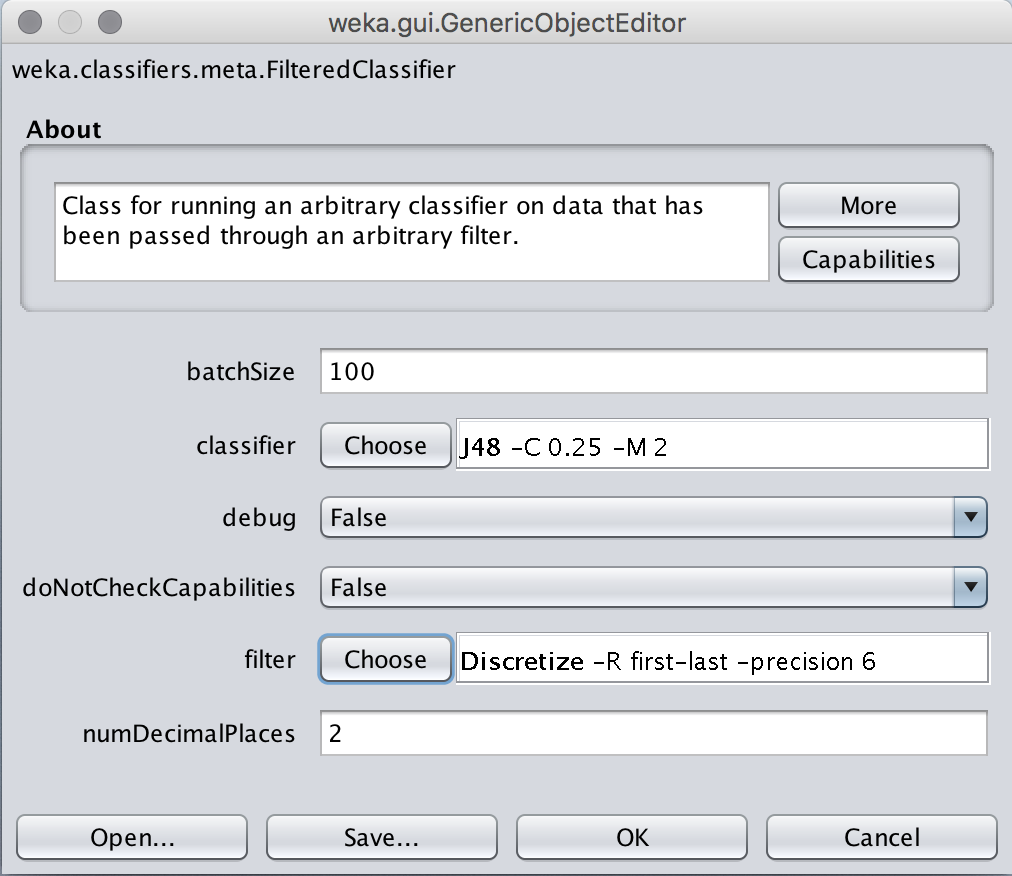
\includegraphics[width=0.45\textwidth]{images/B2_17a.png}}
\qquad
\subfloat[The menu of filters.]{\label{subfig:filtered_classifier_2}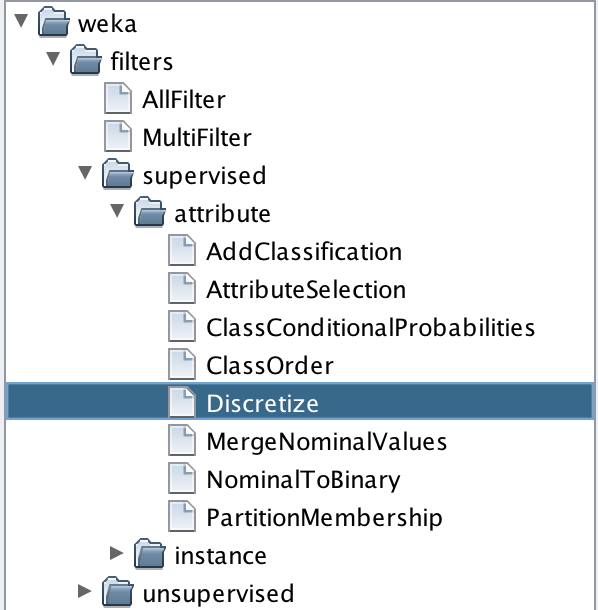
\includegraphics[width=0.45\textwidth]{images/B2_17b.png}}
\caption{\label{fig:filtered_classifier}Using WEKA's metalearner for discretization.}
\end{figure}

Because of popular demand, WEKA allows you to invoke supervised
filters as a preprocessing operation, just like unsupervised
filters. However, if you intend to use them for classification you
should adopt a different methodology. A \textit{metalearner} is
provided so that the process of building the filtering model becomes
part of the learning process. This filters the test data using the
filter that has been created from the training data. It is also useful
for some unsupervised filters. For example, in
\textit{StringToWordVector} the dictionary will be created from the
training data alone: words that are novel in the test data will be
discarded. To use a supervised filter in this way, invoke the
\textit{FilteredClassifier} metalearning scheme from the
\textit{meta} section of the menu displayed by the Classify panel's
Choose button. Figure~\ref{subfig:filtered_classifier_1} shows the
object editor for this metalearning scheme. With it you choose a
classifier and a filter. Figure~\ref{subfig:filtered_classifier_2}
shows the menu of filters.

Supervised filters, just like unsupervised ones, are divided into
attribute and instance filters.

\subsubsection{Supervised attribute filters}

\textit{Discretize}, highlighted in
Figure~\ref{fig:filtered_classifier}, uses the MDL method of
supervised discretization. You can specify a range of attributes or
force the discretized attribute to be binary. The class must be
nominal. By default Fayyad and Irani's (1993) criterion is used, but
Kononenko's method (1995) is an option.

There is a supervised version of the \textit{NominalToBinary} filter
that transforms all multivalued nominal attributes to binary ones. In
this version, the transformation depends on whether the class is
nominal or numeric. If nominal, the same method as before is used: an
attribute with \textit{k} values is transformed into \textit{k} binary
attributes. If the class is numeric, however, the method described in
used by the model tree learner M5' is applied. In either case the class itself is
not transformed.

\textit{ClassOrder} changes the ordering of the class values. The user
determines whether the new ordering is random or in ascending or
descending class frequency. This filter must not be used with the
\textit{FilteredClassifier} metalearning scheme!

\textit{AddClassification} adds to the data the predictions of a given
classifier, which can be either trained on the input dataset or loaded
from a file as a serialized object. New attributes can be added that
hold the predicted class value, the predicted probability distribution
(if the class is nominal), or a flag that indicates misclassified
instances (or, for numeric classes, the difference between the
predicted and actual class values).

\textit{AttributeSelection} applies a given attribute selection
technique in order to reduce the number of attributes in the data. The
user can choose which attribute or subset evaluator to use and combine
it with a search strategy in order to implement an attribute selection
method.

\textit{ClassConditionalProbabilities} converts the values of nominal
and numeric attributes into class conditional probability
estimates. For each original attribute $A$ converted, it creates as many
new attributes as there are class values, where the value of the new
attribute corresponding to class $C_k$ is $P(A | C_k)$. This is essentially the same as what the
naive Bayes classifier computes and, in fact, the implementation uses
naive Bayes internally. Like the unsupervised filters that merge
nominal values, this filter can help when dealing with nominal
attributes that have a large number of distinct values.

\subsubsection{Supervised instance filters}

There are four supervised instance filters. \textit{Resample} is like
the eponymous unsupervised instance filter except that it maintains
the class distribution in the subsample. Alternatively, it can be
configured to bias the class distribution towards a uniform
one. Sampling can be performed with (default) or without
replacement. \textit{SpreadSubsample} also produces a random
subsample, but the frequency difference between the rarest and the
most common class can be controlled---for example, you can specify at
most a 2 : 1 difference in class frequencies. You can also limit the
number of instances in any class by specifying an explicit maximum
count.

\textit{SMOTE} is another filter that samples the data and alters the
class distribution (Chawla et al., 2002). Like
\textit{SpreadSubsample}, it can be used to adjust the relative
frequency between minority and majority classes in the data---but it
takes care not to undersample majority classes and it oversamples the
minority class by creating synthetic instances using a
\textit{k}-nearest neighbor approach. The user can specify the
oversampling percentage and the number of neighbors to use when
creating synthetic instances.

Like the unsupervised instance filter \textit{RemoveFolds},
\textit{StratifiedRemoveFolds} outputs a specified cross-validation
fold for the dataset, except that this time the fold is stratified.

\section{Learning algorithms}

On the \textit{Classify} panel, when you select a learning algorithm
using the \textit{Choose} button the command-line version of the
classifier appears in the line beside the button, including the
parameters specified with minus signs. To change them, click that line
to get an appropriate object editor. The classifiers in WEKA are
divided into Bayesian classifiers, trees, rules, functions, lazy
classifiers and a final miscellaneous category. We describe them
briefly here, along with their parameters. To learn more, choose one
in the WEKA Explorer interface and examine its object editor. A
further kind of classifier, the metalearner, is described in the next
section.

\subsection{Bayesian classifiers}

\textit{NaiveBayes} implements the probabilistic Naive Bayes
classifier. \textit{NaiveBayesSimple} uses the normal distribution to
model numeric attributes. \textit{NaiveBayes} can use kernel density
estimators, which improve performance if the normality assumption is
grossly incorrect; it can also handle numeric attributes using
supervised discretization.

\begin{figure}[!p]
%\centering
\begin{mdframed}[innermargin=-1.5cm]
\begin{Verbatim}[fontsize=\scriptsize]
=== Run information ===

Scheme:       weka.classifiers.bayes.NaiveBayes 
Relation:     weather
Instances:    14
Attributes:   5
              outlook
              temperature
              humidity
              windy
              play
Test mode:    10-fold cross-validation

=== Classifier model (full training set) ===

Naive Bayes Classifier

                 Class
Attribute          yes      no
                (0.63)  (0.38)
===============================
outlook
  sunny             3.0     4.0
  overcast          5.0     1.0
  rainy             4.0     3.0
  [total]          12.0     8.0

temperature
  mean          72.9697 74.8364
  std. dev.      5.2304   7.384
  weight sum          9       5
  precision      1.9091  1.9091

humidity
  mean          78.8395 86.1111
  std. dev.      9.8023  9.2424
  weight sum          9       5
  precision      3.4444  3.4444

windy
  TRUE              4.0     4.0
  FALSE             7.0     3.0
  [total]          11.0     7.0



Time taken to build model: 0 seconds

=== Stratified cross-validation ===
=== Summary ===

Correctly Classified Instances           9               64.2857 %
Incorrectly Classified Instances         5               35.7143 %
Kappa statistic                          0.1026
Mean absolute error                      0.4649
Root mean squared error                  0.543 
Relative absolute error                 97.6254 %
Root relative squared error            110.051  %
Total Number of Instances               14     

=== Detailed Accuracy By Class ===

                 TP Rate  FP Rate  Precision  Recall   F-Measure  MCC      ROC Area  PRC Area  Class
                 0.889    0.800    0.667      0.889    0.762      0.122    0.444     0.633     yes
                 0.200    0.111    0.500      0.200    0.286      0.122    0.444     0.397     no
Weighted Avg.    0.643    0.554    0.607      0.643    0.592      0.122    0.444     0.548     

=== Confusion Matrix ===

 a b   <-- classified as
 8 1 | a = yes
 4 1 | b = no
\end{Verbatim}
\end{mdframed}
\caption{\label{fig:naive_bayes_output}Output of \textit{NaiveBayes} for the weather data.}
\end{figure}

Figure~\ref{fig:naive_bayes_output} shows the output of
\textit{NaiveBayes} on the weather data. The salient difference
between this and the output in Figure~\ref{fig:j48_output} of
\textit{J48} on the same data is that instead of a tree in textual
form, here the parameters of the \textit{Naive Bayes} model are
presented in a table. The first column shows attributes and the other
two show class values; entries are either frequency counts of nominal
values or parameters of normal distributions for numeric
attributes. For example, Figure~\ref{fig:naive_bayes_output} shows
that the mean temperature value for instances of class yes is 72.9697,
while for instances for which $windy = yes$ the values \textit{true}
and \textit{false} occur 4 and 7 times respectively. The grand total
of the yes and no counts for \textit{windy} is, surprisingly,
18---more than the 14 instances in the weather data (the situation for
\textit{outlook} is even worse, totaling 20). The reason is that
\textit{NaiveBayes} avoids zero frequencies by applying the Laplace
correction, which involves initializing each count to 1 rather than to
0.

\textit{NaiveBayesUpdateable} is an incremental version that processes
one instance at a time; it can use a kernel estimator but not
discretization. \textit{NaiveBayesMultinomial} implements the
multinomial Bayes classifier; \textit{NaiveBayesMultinomialUpdateable}
is an incremental version. \textit{NaiveBayesMultinomialText} is a
version of incremental multinomial naive Bayes that can work directly
on string attributes. It effectively performs the function of the
\textit{StringToWordVector} filter, minus the TF/IDF transformation,
on the fly.

\textit{BayesNet} learns Bayesian nets under the assumptions made in
Section 6.7: nominal attributes (numeric ones are prediscretized) and
no missing values (any such values are replaced globally). There are
four different algorithms for estimating the conditional probability
tables of the network. Search is done using the K2 or the TAN
algorithms, or more sophisticated methods based on hill-climbing,
simulated annealing, tabu search, and genetic algorithms. Optionally
search speed can be improved using AD trees. There are also two
algorithms that use conditional independence tests to learn the
structure of the network; alternatively, the network structure can be
loaded from an XML file. More details on the implementation of
Bayesian networks in WEKA can be found in Bouckaert (2004).

\begin{figure}[!th]
\centering
\subfloat[Default outpuit.]{\label{subfig:bayes_net_1}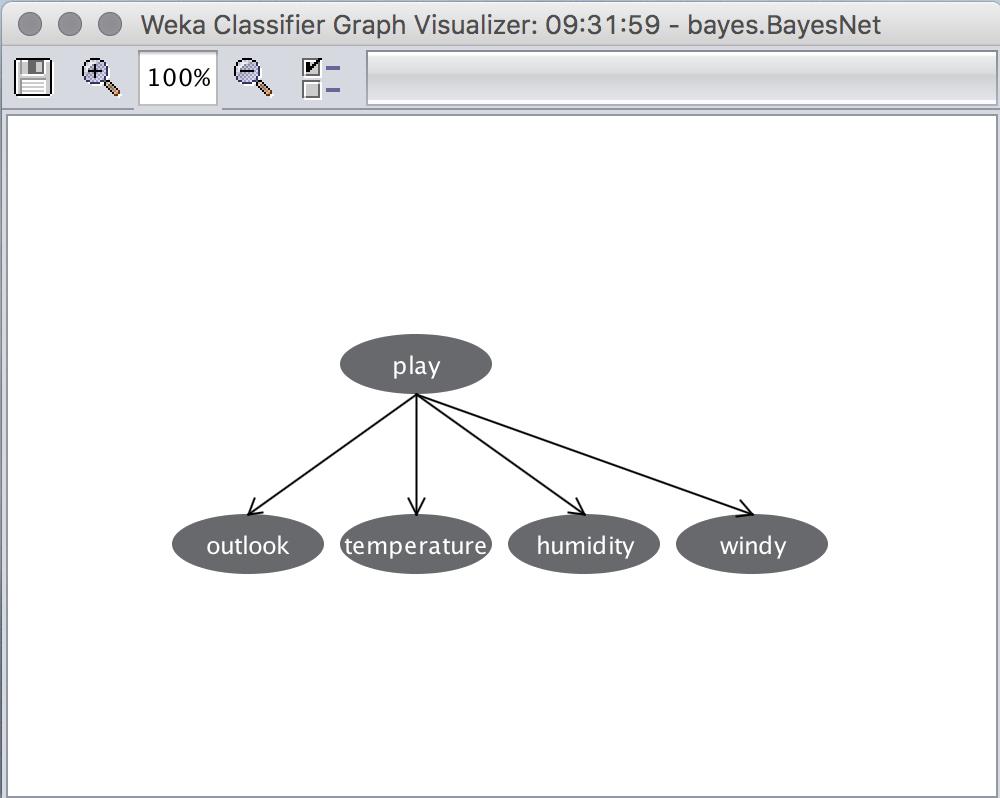
\includegraphics[width=0.45\textwidth]{images/B2_19a.png}}
\qquad
\subfloat[Maximum number of parents set to three in the search algorithm.]{\label{subfig:bayes_net_2}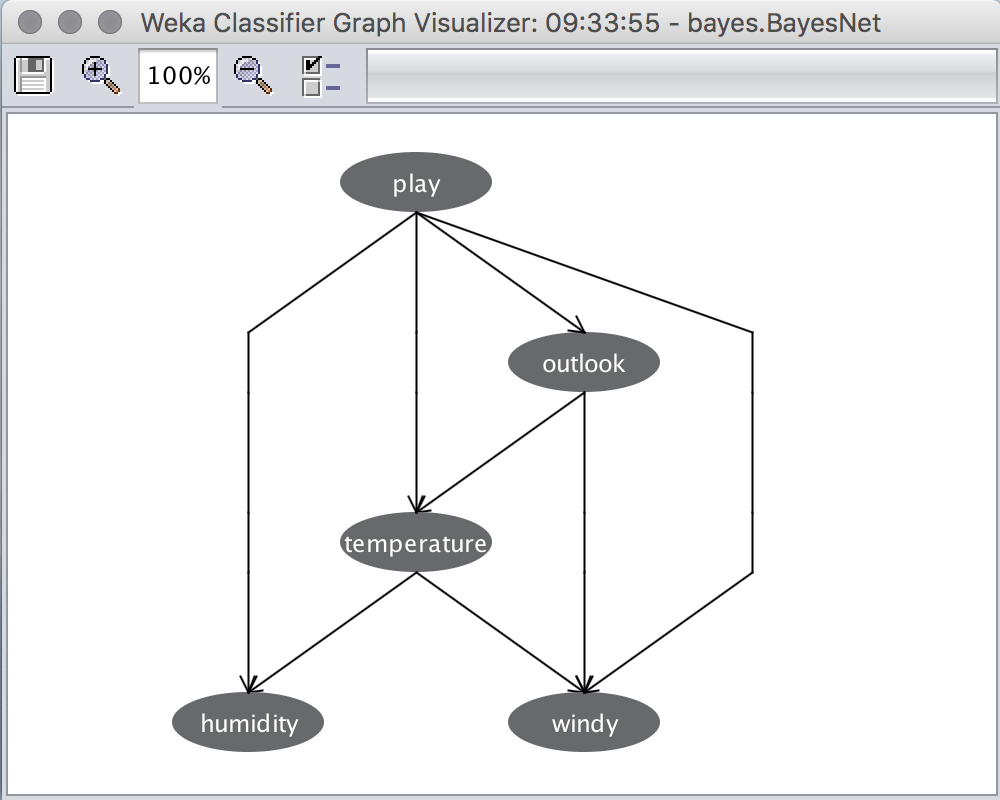
\includegraphics[width=0.45\textwidth]{images/B2_19b.png}}
\newline
\subfloat[The probability distribution table for the windy node in (b).]{\label{subfig:bayes_net_3}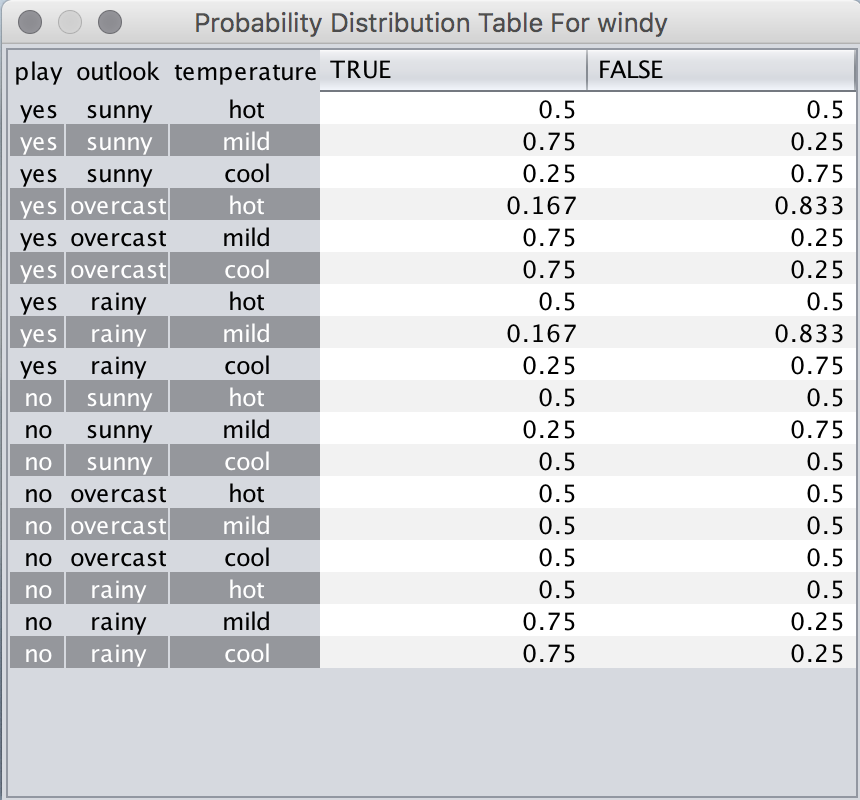
\includegraphics[width=0.45\textwidth]{images/B2_19c.png}}
\caption{\label{fig:weather}Visualizing a Bayesian network for the weather data (nominal version).}
\end{figure}

You can observe the network structure by right-clicking the history
item and selecting Visualize graph. Figure~\ref{subfig:bayes_net_1}
shows the graph for the nominal version of the weather data, which in
fact corresponds to the Naive Bayes result with all probabilities
conditioned on the class value. This is because the search algorithm
defaults to K2 with the maximum number of parents of a node set to
one. Reconfiguring this to three by clicking on K2 in the
configuration panel yields the more interesting network in
Figure~\ref{subfig:bayes_net_2}. Clicking on a node shows its
probability distribution---Figure~\ref{subfig:bayes_net_3} is obtained
by clicking on the windy node in Figure~\ref{subfig:bayes_net_2}.

\subsection{Trees}

\begin{figure}[!th]
\centering
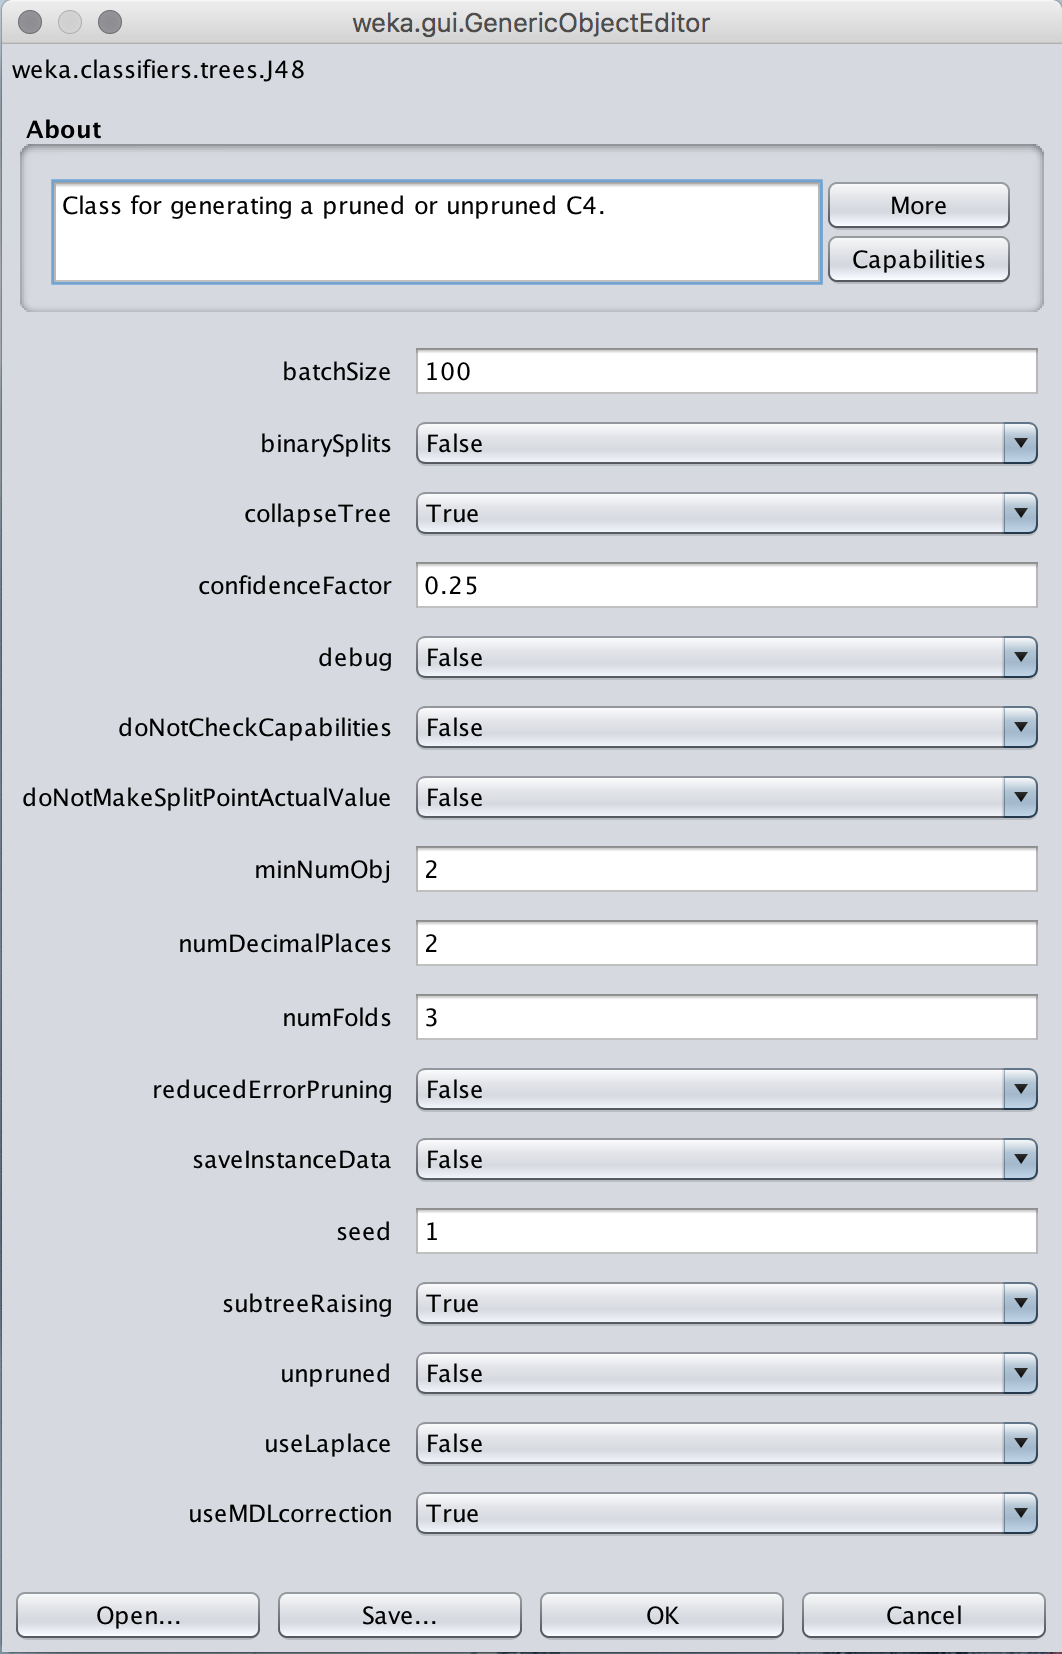
\includegraphics[width=0.6\textwidth]{images/B2_20.png}
\caption{Changing the parameters for J4.8.}
\label{fig:goe_j48}
\end{figure}

Of the tree classifiers in WEKA, we have already seen how to use J4.8,
which reimplements C4.5. To see the options, click the line beside the
\textit{Choose} button in Figure~\ref{subfig:j48_2} to bring up the
object editor in Figure~\ref{fig:goe_j48}. You can build a binary tree
instead of one with multiway branches. You can set the confidence
threshold for pruning (default 0.25), and the minimum number of
instances permissible at a leaf (default 2). Instead of standard C4.5
pruning you can choose reduced-error pruning. The \textit{numFolds}
parameter (default 3) determines the size of the pruning set: the data
is divided equally into that number of parts and the last one used for
pruning. When visualizing the tree it is nice to be able to consult
the original data points, which you can do if
\textit{saveInstanceData} has been turned on (it is off, or
\textit{False}, by default to reduce memory requirements). You can
suppress subtree raising, yielding a more efficient algorithm; force
the algorithm to use the unpruned tree instead of the pruned one; or
use Laplace smoothing for predicted probabilities.

\textit{DecisionStump}, designed for use with the boosting methods
described later, builds one-level binary decision trees for datasets
with a categorical or numeric class, dealing with missing values by
treating them as a separate value and extending a third branch from
the stump. Trees built by \textit{RandomTree} consider a given number of
random features at each node, performing no
pruning. \textit{RandomForest} constructs random forests by bagging
ensembles of random trees.

\textit{REPTree} builds a decision or regression tree using
information gain/variance reduction and prunes it using reduced-error
pruning. Optimized for speed, it only sorts values for numeric
attributes once. It deals with missing values
by splitting instances into pieces, as C4.5 does. You can set the
minimum number of instances per leaf, maximum tree depth (useful when
boosting trees), minimum proportion of training set variance for a
split (numeric classes only), and number of folds for pruning.

\textit{M5P} is the model tree learner M5$\prime$ described in Chapter 7 of the book.

\textit{LMT} builds logistic model trees. It can deal with binary and
multiclass target variables, numeric and nominal attributes, and
missing values. When fitting the logistic regression functions at a
node using the \textit{LogitBoost} algorithm, it uses cross-validation
to determine how many iterations to run just once and employs the same
number throughout the tree instead of cross-validating at every
node. This heuristic (which you can switch off) improves the run time
considerably, with little effect on accuracy. Alternatively, you can
set the number of boosting iterations to be used throughout the tree
manually, or use a fast heuristic based on the Akaike Information
Criterion instead of cross-validation. Weight trimming during the
boosting process can be used to further improve run time. Normally, it
is the misclassification error that cross-validation minimizes, but
the mean absolute error of the probability estimates can be chosen
instead. The splitting criterion can be based on C4.5's information
gain (the default) or on the LogitBoost residuals, striving to improve
the purity of the residuals. LMT employs the minimal cost-complexity
pruning mechanism to produce a compact tree structure.

\textit{HoeffdingTree} is an implementation of the incremental decision tree
algorithm algorithm described in Chapter 13 of the book. It offers options to
create splits based on information gain or the Gini index. Predictions
at the leaves of the tree can be made by either majority class or
naive Bayes models.

\subsection{Rules}

\textit{DecisionTable} builds a decision table classifier. It
evaluates feature subsets using best-first search and can use
cross-validation for evaluation (Kohavi 1995b). An option uses the
nearest-neighbor method to determine the class for each instance that
is not covered by a decision table entry, instead of the table's
global majority, based on the same set of features.

\begin{figure}[!p]
%\centering
\begin{mdframed}[innermargin=-1.5cm]
\begin{Verbatim}[fontsize=\scriptsize]
=== Run information ===

Scheme:       weka.classifiers.rules.OneR -B 6
Relation:     labor-neg-data
Instances:    57
Attributes:   17
              duration
              wage-increase-first-year
              wage-increase-second-year
              wage-increase-third-year
              cost-of-living-adjustment
              working-hours
              pension
              standby-pay
              shift-differential
              education-allowance
              statutory-holidays
              vacation
              longterm-disability-assistance
              contribution-to-dental-plan
              bereavement-assistance
              contribution-to-health-plan
              class
Test mode:    10-fold cross-validation

=== Classifier model (full training set) ===

wage-increase-first-year:
< 2.9-> bad
>= 2.9-> good
?-> good
(48/57 instances correct)


Time taken to build model: 0 seconds

=== Stratified cross-validation ===
=== Summary ===

Correctly Classified Instances          41               71.9298 %
Incorrectly Classified Instances        16               28.0702 %
Kappa statistic                          0.3382
Mean absolute error                      0.2807
Root mean squared error                  0.5298
Relative absolute error                 61.3628 %
Root relative squared error            110.9627 %
Total Number of Instances               57     

=== Detailed Accuracy By Class ===

                 TP Rate  FP Rate  Precision  Recall   F-Measure  MCC      ROC Area  PRC Area  Class
                 0.450    0.135    0.643      0.450    0.529      0.349    0.657     0.482     bad
                 0.865    0.550    0.744      0.865    0.800      0.349    0.657     0.731     good
Weighted Avg.    0.719    0.404    0.709      0.719    0.705      0.349    0.657     0.644     

=== Confusion Matrix ===

  a  b   <-- classified as
  9 11 |  a = bad
  5 32 |  b = good
\end{Verbatim}
\end{mdframed}
\caption{\label{fig:oneR_output}Output of \textit{OneR} for the labor negotiations data.}
\end{figure}

\textit{OneR} is the 1R classifier with one parameter: the minimum
bucket size for discretization. Figure~\ref{fig:oneR_output} shows its
output for the labor negotiations data. The Classifier model part
shows that wage-increase-first-year has been identified as the basis
of the rule produced, with a split at the value 2.9 dividing bad
outcomes from good ones (the class is also good if the value of that
attribute is missing). Beneath the rules the fraction of training
instances correctly classified by the rules is given in parentheses.

\begin{figure}[!p]
%\centering
\begin{mdframed}[innermargin=-1.5cm]
\begin{Verbatim}[fontsize=\scriptsize]
=== Run information ===

Scheme:       weka.classifiers.rules.PART -M 2 -C 0.25 -Q 1
Relation:     labor-neg-data
Instances:    57
Attributes:   17
              duration
              wage-increase-first-year
              wage-increase-second-year
              wage-increase-third-year
              cost-of-living-adjustment
              working-hours
              pension
              standby-pay
              shift-differential
              education-allowance
              statutory-holidays
              vacation
              longterm-disability-assistance
              contribution-to-dental-plan
              bereavement-assistance
              contribution-to-health-plan
              class
Test mode:    10-fold cross-validation

=== Classifier model (full training set) ===

PART decision list
------------------

wage-increase-first-year > 2.5 AND
longterm-disability-assistance = yes AND
statutory-holidays > 10: good (25.67)

wage-increase-first-year <= 4 AND
working-hours > 36: bad (19.4/1.58)

: good (11.93/2.18)

Number of Rules  : 3


Time taken to build model: 0.01 seconds

=== Stratified cross-validation ===
=== Summary ===

Correctly Classified Instances          45               78.9474 %
Incorrectly Classified Instances        12               21.0526 %
Kappa statistic                          0.5378
Mean absolute error                      0.2884
Root mean squared error                  0.4339
Relative absolute error                 63.0507 %
Root relative squared error             90.8836 %
Total Number of Instances               57     

=== Detailed Accuracy By Class ===

                 TP Rate  FP Rate  Precision  Recall   F-Measure  MCC      ROC Area  PRC Area  Class
                 0.700    0.162    0.700      0.700    0.700      0.538    0.726     0.613     bad
                 0.838    0.300    0.838      0.838    0.838      0.538    0.726     0.758     good
Weighted Avg.    0.789    0.252    0.789      0.789    0.789      0.538    0.726     0.707     

=== Confusion Matrix ===

  a  b   <-- classified as
 14  6 |  a = bad
  6 31 |  b = good
\end{Verbatim}
\end{mdframed}
\caption{\label{fig:part_output}Output of \textit{Part} for the labor negotiations data.}
\end{figure}

\textit{Part} obtains rules from partial decision trees. It builds the
tree using C4.5's heuristics with the same user-defined parameters as
J4.8. Figure~\ref{fig:part_output} shows the output of Part for the
labor negotiations data. Three rules are found, and are intended to be
processed in order, the prediction generated for any test instance
being the outcome of the first rule that fires. The last, ``catch-all,''
rule will always fire if no other rule fires. As with J48, the numbers in parentheses that
follow each rule give the number of instances that are covered by the
rule followed by the number that are misclassified (if any).

\textit{M5Rules} obtains regression rules from model trees built using
M5'. \textit{Ridor} learns rules with exceptions by generating the
default rule, using incremental reduced-error pruning to find
exceptions with the smallest error rate, finding the best exceptions
for each exception, and iterating.

\textit{JRip} implements Ripper algorithm, including heuristic global
optimization of the rule set (Cohen 1995). \textit{NNge} is a
nearest-neighbor method for generating rules using nonnested
generalized exemplars.

\subsection{Functions}

\begin{figure}[!hp]
%\centering
\begin{mdframed}[innermargin=-1.5cm]
\begin{Verbatim}[fontsize=\footnotesize]
=== Run information ===

Scheme:       weka.classifiers.functions.SimpleLinearRegression 
Relation:     cpu
Instances:    209
Attributes:   7
              MYCT
              MMIN
              MMAX
              CACH
              CHMIN
              CHMAX
              class
Test mode:    10-fold cross-validation

=== Classifier model (full training set) ===

Linear regression on MMAX

0.01 * MMAX - 34

Predicting 0 if attribute value is missing.


Time taken to build model: 0 seconds

=== Cross-validation ===
=== Summary ===

Correlation coefficient                  0.7844
Mean absolute error                     53.8054
Root mean squared error                 99.5674
Relative absolute error                 55.908  %
Root relative squared error             61.8997 %
Total Number of Instances              209 
\end{Verbatim}
\end{mdframed}
\caption{\label{fig:simple_linear_regression_output}Output of \textit{SimpleLinearRegression} on the CPU performance data.}
\end{figure}

Algorithms that fall into the \textit{functions} category include an
assorted group of classifiers that can be written down as mathematical
equations in a reasonably natural way. Other methods, such as decision
trees and rules, cannot (there are exceptions: Naive Bayes has a
simple mathematical formulation). Four of them implement linear
regression. \textit{SimpleLinearRegression} learns a linear regression
model based on a single attribute---it chooses the one that yields the
smallest squared error. Missing values and nonnumeric attributes are
not allowed. Figure~\ref{fig:simple_linear_regression_output} shows
the output of \textit{SimpleLinearRegression} for the CPU performance
data. The attribute that has the smallest squared error in this case
is \textit{MMAX}.

\textit{LinearRegression} performs least-squares multiple
linear regression including attribute selection,
either greedily using backward elimination or by building a full model
from all attributes and dropping terms one by one in decreasing order
of their standardized coefficients until a stopping criteria is
reached. Both methods use a version of the AIC termination
criterion. Attribute selection can be turned off. The implementation has two further refinements: a heuristic
mechanism for detecting collinear attributes (which can be turned off)
and a ridge parameter that stabilizes degenerate cases and can reduce
overfitting by penalizing large coefficients. Technically,
\textit{LinearRegression} implements ridge regression.

\textit{SMO} implements the sequential minimal optimization algorithm for
training a support vector classifier (Platt, 1998; Keerthi
et al., 2001), using kernel
functions such as polynomial or Gaussian kernels. Missing values are replaced globally, nominal
attributes are transformed into binary ones, and attributes are
normalized by default---note that the coefficients in the output are
based on the normalized data. Normalization can be turned off, or the
input standardized to zero mean and unit variance. Pairwise
classification is used for multiclass problems. Logistic regression
models can be fitted to the support vector machine output to obtain
probability estimates. In the multiclass case the predicted
probabilities will be combined using pairwise coupling (Hastie and
Tibshirani, 1998). When working with sparse instances, turn
normalization off for faster operation.

\begin{figure}[!p]
%\centering
\begin{mdframed}[innermargin=-1.0cm]
\begin{Verbatim}[fontsize=\tiny]
=== Run information ===

Scheme:       weka.classifiers.functions.SMO -C 1.0 -L 0.001 -P 1.0E-12 -N 0 -V -1 -W 1 
              -K ``weka.classifiers.functions.supportVector.PolyKernel -E 1.0 -C 250007'' 
              -calibrator ``weka.classifiers.functions.Logistic -R 1.0E-8 -M -1 -num-decimal-places 4''
Relation:     iris
Instances:    150
Attributes:   5
              sepallength
              sepalwidth
              petallength
              petalwidth
              class
Test mode:    10-fold cross-validation

=== Classifier model (full training set) ===

SMO

Kernel used:
  Linear Kernel: K(x,y) = <x,y>

Classifier for classes: Iris-setosa, Iris-versicolor

BinarySMO
Machine linear: showing attribute weights, not support vectors.

         0.6829 * (normalized) sepallength
 +      -1.523  * (normalized) sepalwidth
 +       2.2034 * (normalized) petallength
 +       1.9272 * (normalized) petalwidth
 -       0.7091

Number of kernel evaluations: 352 (70.32% cached)

Classifier for classes: Iris-setosa, Iris-virginica

BinarySMO
Machine linear: showing attribute weights, not support vectors.

         0.5886 * (normalized) sepallength
 +      -0.5782 * (normalized) sepalwidth
 +       1.6429 * (normalized) petallength
 +       1.4777 * (normalized) petalwidth
 -       1.1668

Number of kernel evaluations: 284 (68.996% cached)

Classifier for classes: Iris-versicolor, Iris-virginica

BinarySMO
Machine linear: showing attribute weights, not support vectors.

         0.3176 * (normalized) sepallength
 +      -0.863  * (normalized) sepalwidth
 +       3.0543 * (normalized) petallength
 +       4.0815 * (normalized) petalwidth
 -       4.5924

Number of kernel evaluations: 453 (61.381% cached)

Time taken to build model: 0.03 seconds

=== Stratified cross-validation ===
=== Summary ===

Correctly Classified Instances         144               96      %
Incorrectly Classified Instances         6                4      %
Kappa statistic                          0.94  
Mean absolute error                      0.2311
Root mean squared error                  0.288 
Relative absolute error                 52      %
Root relative squared error             61.101  %
Total Number of Instances              150     

=== Detailed Accuracy By Class ===

                 TP Rate  FP Rate  Precision  Recall   F-Measure  MCC      ROC Area  PRC Area  Class
                 1.000    0.000    1.000      1.000    1.000      1.000    1.000     1.000     Iris-setosa
                 0.980    0.050    0.907      0.980    0.942      0.913    0.965     0.896     Iris-versicolor
                 0.900    0.010    0.978      0.900    0.938      0.910    0.970     0.930     Iris-virginica
Weighted Avg.    0.960    0.020    0.962      0.960    0.960      0.941    0.978     0.942     

=== Confusion Matrix ===

  a  b  c   <-- classified as
 50  0  0 |  a = Iris-setosa
  0 49  1 |  b = Iris-versicolor
  0  5 45 |  c = Iris-virginica
\end{Verbatim}
\end{mdframed}
\caption{\label{fig:smo_output}Output of \textit{SMO} on the iris data.}
\end{figure}

\begin{figure}[!p]
%\centering
\begin{mdframed}[innermargin=-1.0cm]
\begin{Verbatim}[fontsize=\tiny]
=== Run information ===

Scheme:       weka.classifiers.functions.SMO -C 1.0 -L 0.001 -P 1.0E-12 -N 0 -V -1 -W 1 
              -K ``weka.classifiers.functions.supportVector.PolyKernel -E 2.0 -C 250007'' 
              -calibrator ``weka.classifiers.functions.Logistic -R 1.0E-8 -M -1 -num-decimal-places 4''
Relation:     iris
Instances:    150
Attributes:   5
              sepallength
              sepalwidth
              petallength
              petalwidth
              class
Test mode:    10-fold cross-validation

=== Classifier model (full training set) ===

SMO

Kernel used:
  Poly Kernel: K(x,y) = <x,y>^2.0

Classifier for classes: Iris-setosa, Iris-versicolor

BinarySMO

      1      * <0.333333 0.166667 0.457627 0.375 > * X]
 -       1      * <0.222222 0.541667 0.118644 0.166667 > * X]
 -       1      * <0.138889 0.416667 0.067797 0.083333 > * X]
 -       1      * <0.166667 0.416667 0.067797 0.041667 > * X]
 +       1      * <0.222222 0.208333 0.338983 0.416667 > * X]
 -       1      * <0.055556 0.125 0.050847 0.083333 > * X]
 -       1      * <0.027778 0.375 0.067797 0.041667 > * X]
 +       1      * <0.166667 0.166667 0.389831 0.375 > * X]
 +       1      * <0.361111 0.208333 0.491525 0.416667 > * X]
 +       1      * <0.194444 0 0.423729 0.375 > * X]
 -       1      * <0.194444 0.416667 0.101695 0.041667 > * X]
 -       1      * <0.138889 0.458333 0.101695 0.041667 > * X]
 +       1      * <0.194444 0.125 0.389831 0.375 > * X]
 +       0.3697 * <0.361111 0.375 0.440678 0.5 > * X]
 -       0.4599 * <0.138889 0.416667 0.067797 0 > * X]
 -       0.9098 * <0.194444 0.625 0.101695 0.208333 > * X]
 +       1      * <0.333333 0.166667 0.474576 0.416667 > * X]
 +       1      * <0.388889 0.25 0.423729 0.375 > * X]
 -       0.8085

Number of support vectors: 18

Number of kernel evaluations: 2416 (72.564% cached)

Classifier for classes: Iris-setosa, Iris-virginica

BinarySMO
      1      * <0.166667 0.208333 0.59322 0.666667 > * X]
 -       0.856  * <0.055556 0.125 0.050847 0.083333 > * X]
 +       0.1315 * <0.555556 0.333333 0.694915 0.583333 > * X]
 -       1      * <0.222222 0.541667 0.118644 0.166667 > * X]
 +       1      * <0.472222 0.083333 0.677966 0.583333 > * X]
 -       0.2756 * <0.194444 0.625 0.101695 0.208333 > * X]
 -       1.0183

Number of support vectors: 6

Number of kernel evaluations: 1364 (60.726% cached)

Classifier for classes: Iris-versicolor, Iris-virginica

BinarySMO
      1      * <0.555556 0.208333 0.677966 0.75 > * X]
 -       1      * <0.305556 0.416667 0.59322 0.583333 > * X]
 -       1      * <0.666667 0.458333 0.627119 0.583333 > * X]
 -       1      * <0.472222 0.583333 0.59322 0.625 > * X]
 +       1      * <0.444444 0.416667 0.694915 0.708333 > * X]
 -       1      * <0.527778 0.083333 0.59322 0.583333 > * X]
 +       1      * <0.416667 0.291667 0.694915 0.75 > * X]
 -       1      * <0.472222 0.291667 0.694915 0.625 > * X]
 +       0.4559 * <0.555556 0.375 0.779661 0.708333 > * X]
 -       1      * <0.666667 0.416667 0.677966 0.666667 > * X]
 +       1      * <0.611111 0.416667 0.762712 0.708333 > * X]
 -       1      * <0.5 0.375 0.627119 0.541667 > * X]
 -       1      * <0.722222 0.458333 0.661017 0.583333 > * X]
 +       1      * <0.472222 0.083333 0.677966 0.583333 > * X]
 +       1      * <0.583333 0.458333 0.762712 0.708333 > * X]
 +       1      * <0.611111 0.5 0.694915 0.791667 > * X]
 +       1      * <0.5 0.416667 0.661017 0.708333 > * X]
 -       1      * <0.694444 0.333333 0.644068 0.541667 > * X]
 -       1      * <0.5 0.416667 0.610169 0.541667 > * X]
 +       1      * <0.416667 0.291667 0.694915 0.75 > * X]
 +       1      * <0.527778 0.333333 0.644068 0.708333 > * X]
 -       1      * <0.444444 0.5 0.644068 0.708333 > * X]
 +       1      * <0.5 0.25 0.779661 0.541667 > * X]
 +       1      * <0.555556 0.291667 0.661017 0.708333 > * X]
 +       1      * <0.361111 0.333333 0.661017 0.791667 > * X]
 -       1      * <0.555556 0.208333 0.661017 0.583333 > * X]
 -       0.4559 * <0.555556 0.125 0.576271 0.5 > * X]
 +       1      * <0.555556 0.333333 0.694915 0.583333 > * X]
 +       1      * <0.166667 0.208333 0.59322 0.666667 > * X]
 +       1      * <0.805556 0.416667 0.813559 0.625 > * X]
 -       1      * <0.555556 0.541667 0.627119 0.625 > * X]
 +       1      * <0.472222 0.416667 0.644068 0.708333 > * X]
 -       1      * <0.361111 0.416667 0.59322 0.583333 > * X]
 -       1      * <0.583333 0.5 0.59322 0.583333 > * X]
 -       1      * <0.472222 0.375 0.59322 0.583333 > * X]
 -       1      * <0.611111 0.333333 0.610169 0.583333 > * X]
 -       3.5378

Number of support vectors: 36

Number of kernel evaluations: 3524 (66.711% cached)

Time taken to build model: 0.01 seconds
\end{Verbatim}
\end{mdframed}
\caption{\label{fig:smo_nonlinear_output}Output of \textit{SMO} with a nonlinear kernel on the iris data.}
\end{figure}

\begin{figure}[!th]
%\centering
\begin{mdframed}[innermargin=-1.0cm]
\begin{Verbatim}[fontsize=\tiny]
=== Stratified cross-validation ===
=== Summary ===

Correctly Classified Instances         144               96      %
Incorrectly Classified Instances         6                4      %
Kappa statistic                          0.94  
Mean absolute error                      0.2311
Root mean squared error                  0.288 
Relative absolute error                 52      %
Root relative squared error             61.101  %
Total Number of Instances              150     

=== Detailed Accuracy By Class ===

                 TP Rate  FP Rate  Precision  Recall   F-Measure  MCC      ROC Area  PRC Area  Class
                 1.000    0.000    1.000      1.000    1.000      1.000    1.000     1.000     Iris-setosa
                 0.940    0.030    0.940      0.940    0.940      0.910    0.955     0.904     Iris-versicolor
                 0.940    0.030    0.940      0.940    0.940      0.910    0.972     0.916     Iris-virginica
Weighted Avg.    0.960    0.020    0.960      0.960    0.960      0.940    0.976     0.940     

=== Confusion Matrix ===

  a  b  c   <-- classified as
 50  0  0 |  a = Iris-setosa
  0 47  3 |  b = Iris-versicolor
  0  3 47 |  c = Iris-virginica
\end{Verbatim}
\end{mdframed}
\caption{\label{fig:smo_nonlinear_cont} Output of \textit{SMO} with a nonlinear kernel on the iris data, cont'd.}
\end{figure}

Figure~\ref{fig:smo_output} shows the output of \textit{SMO} on the
iris data. A polynomial kernel with an exponent of 1 has been used,
making the model a linear support vector machine. Since the iris data
contains three class values, three binary SMO models have been
output---one hyperplane to separate each possible pair of class
values. Furthermore, since the machine is linear, the hyperplanes are
expressed as functions of the attribute values in the original (albeit
normalized) space. Figures~\ref{fig:smo_nonlinear_output} and~\ref{fig:smo_nonlinear_cont} show the result when the exponent of the
polynomial kernel is set to 2, making the support vector machine
nonlinear. There are three binary SMO models as before, but this time
the classifiers are expressed as functions of the support
vectors. Each support vector is shown enclosed in angle brackets,
along with the value of its coefficient $\alpha$. The value of the
offset parameter, $b$, is shown
as the last component of each function.

\textit{SMOreg} implements the sequential minimal optimization algorithm for
learning a support vector regression model (Smola and Schölkopf,
1998).

\textit{VotedPerceptron} is the voted perceptron
algorithm. \textit{Winnow} modifies the basic perceptron to use
multiplicative updates. The implementation allows for a second
multiplier $\beta$---different from $1/\alpha$---to be used, which
makes the algorithm slightly more flexible than the version of
balanced Winnow discussed in the book.

\textit{GaussianProcesses} implements the Bayesian Gaussian process
technique for non-linear regression. Users can specify the kernel
function, along with a ``noise'' regularization parameter for
controlling the closeness of fit. They can choose to have the training
data normalized or standardized before learning the regression. For
point estimates, this method is equivalent to kernel ridge regression.

\textit{SGD} implements stochastic gradient descent learning of linear
models. Models can be learned in either a batch or incremental
fashion. The loss function chosen determines the type of model
learned. Available loss functions include the hinge loss (linear
support vector classifier), log loss (logistic regression), squared
loss (least squares linear regression), epsilon-insensitive loss
(support vector regression) and Huber loss (robust
regression). \textit{SGDText}, like
\textit{NaiveBayesMultinomialText}, is a version that is designed for
text classification and can operate directly on string
attributes. \textit{SGDText} is limited to just the hinge and log
loss.

\textit{SimpleLogistic} builds logistic regression models, fitting
them using LogitBoost with simple regression functions as base
learners and determining how many iterations to perform using
cross-validation---which supports automatic attribute
selection. \textit{SimpleLogistic} generates a degenerate logistic
model tree comprising a single node, and supports the options given
earlier for \textit{LMT}.

\begin{figure}[!th]
%\centering
\begin{mdframed}[innermargin=-1.0cm]
\begin{Verbatim}[fontsize=\tiny]
=== Run information ===

Scheme:       weka.classifiers.functions.Logistic -R 1.0E-8 -M -1 -num-decimal-places 4
Relation:     iris
Instances:    150
Attributes:   5
              sepallength
              sepalwidth
              petallength
              petalwidth
              class
Test mode:    10-fold cross-validation

=== Classifier model (full training set) ===

Logistic Regression with ridge parameter of 1.0E-8
Coefficients...
                         Class
Variable           Iris-setosa  Iris-versicolor
===============================================
sepallength            21.8065           2.4652
sepalwidth              4.5648           6.6809
petallength           -26.3083          -9.4293
petalwidth             -43.887         -18.2859
Intercept               8.1743           42.637


Odds Ratios...
                         Class
Variable           Iris-setosa  Iris-versicolor
===============================================
sepallength    2954196659.8892          11.7653
sepalwidth             96.0426         797.0304
petallength                  0           0.0001
petalwidth                   0                0


Time taken to build model: 0.01 seconds

=== Stratified cross-validation ===
=== Summary ===

Correctly Classified Instances         144               96      %
Incorrectly Classified Instances         6                4      %
Kappa statistic                          0.94  
Mean absolute error                      0.0287
Root mean squared error                  0.1424
Relative absolute error                  6.456  %
Root relative squared error             30.2139 %
Total Number of Instances              150     

=== Detailed Accuracy By Class ===

                 TP Rate  FP Rate  Precision  Recall   F-Measure  MCC      ROC Area  PRC Area  Class
                 1.000    0.000    1.000      1.000    1.000      1.000    1.000     1.000     Iris-setosa
                 0.920    0.020    0.958      0.920    0.939      0.910    0.970     0.933     Iris-versicolor
                 0.960    0.040    0.923      0.960    0.941      0.911    0.975     0.933     Iris-virginica
Weighted Avg.    0.960    0.020    0.960      0.960    0.960      0.940    0.982     0.955     

=== Confusion Matrix ===

  a  b  c   <-- classified as
 50  0  0 |  a = Iris-setosa
  0 46  4 |  b = Iris-versicolor
  0  2 48 |  c = Iris-virginica
\end{Verbatim}
\end{mdframed}
\caption{\label{fig:logistic_output}Output of \textit{Logistic} for the iris data.}
\end{figure}

\textit{Logistic} is an alternative implementation for building and
using a multinomial logistic regression model with a ridge estimator
to guard against overfitting by penalizing large coefficients, based
on work by le Cessie and van Houwelingen
(1992). Figure~\ref{fig:logistic_output} shows its output on the iris
data. The coefficients of the regression functions are shown in
tabular form, one for each class value except for the last
class. Given $m$ input attributes and $k$ classes, the probability
predicted for class $j$ (with the exception of the last class) is given
by\newline

$P(j|a_1,a_2,...,a_m)=\frac{exp(w^j_0+w^j_1a_1+w^j_2a_2+...+w^j_ma_m)}{1 + \sum_{j=1}^{k-1}exp(w^j_0+w^j_1a_1+w^j_2a_2+...+w^j_ma_m)}$\newline

where $w^j_0$ is the intercept term for class $j$. The probability of the last class $k$ is given by\newline

$1-\sum_{j=1}^{k-1}P(j|a_1,a_2,...,a_m)$\newline

Beneath the table of regression coefficients is a second table giving
an estimate of the odds ratio for each input attribute and class
value. For a given attribute, this value gives an indication of its
influence on the class when the values of the other attributes are
held fixed.

\subsection{Neural networks}

\begin{figure}[!th]
\centering
\subfloat[Beginning the process of editing the network to add a second hidden layer.]{\label{subfig:mlp_editor_1}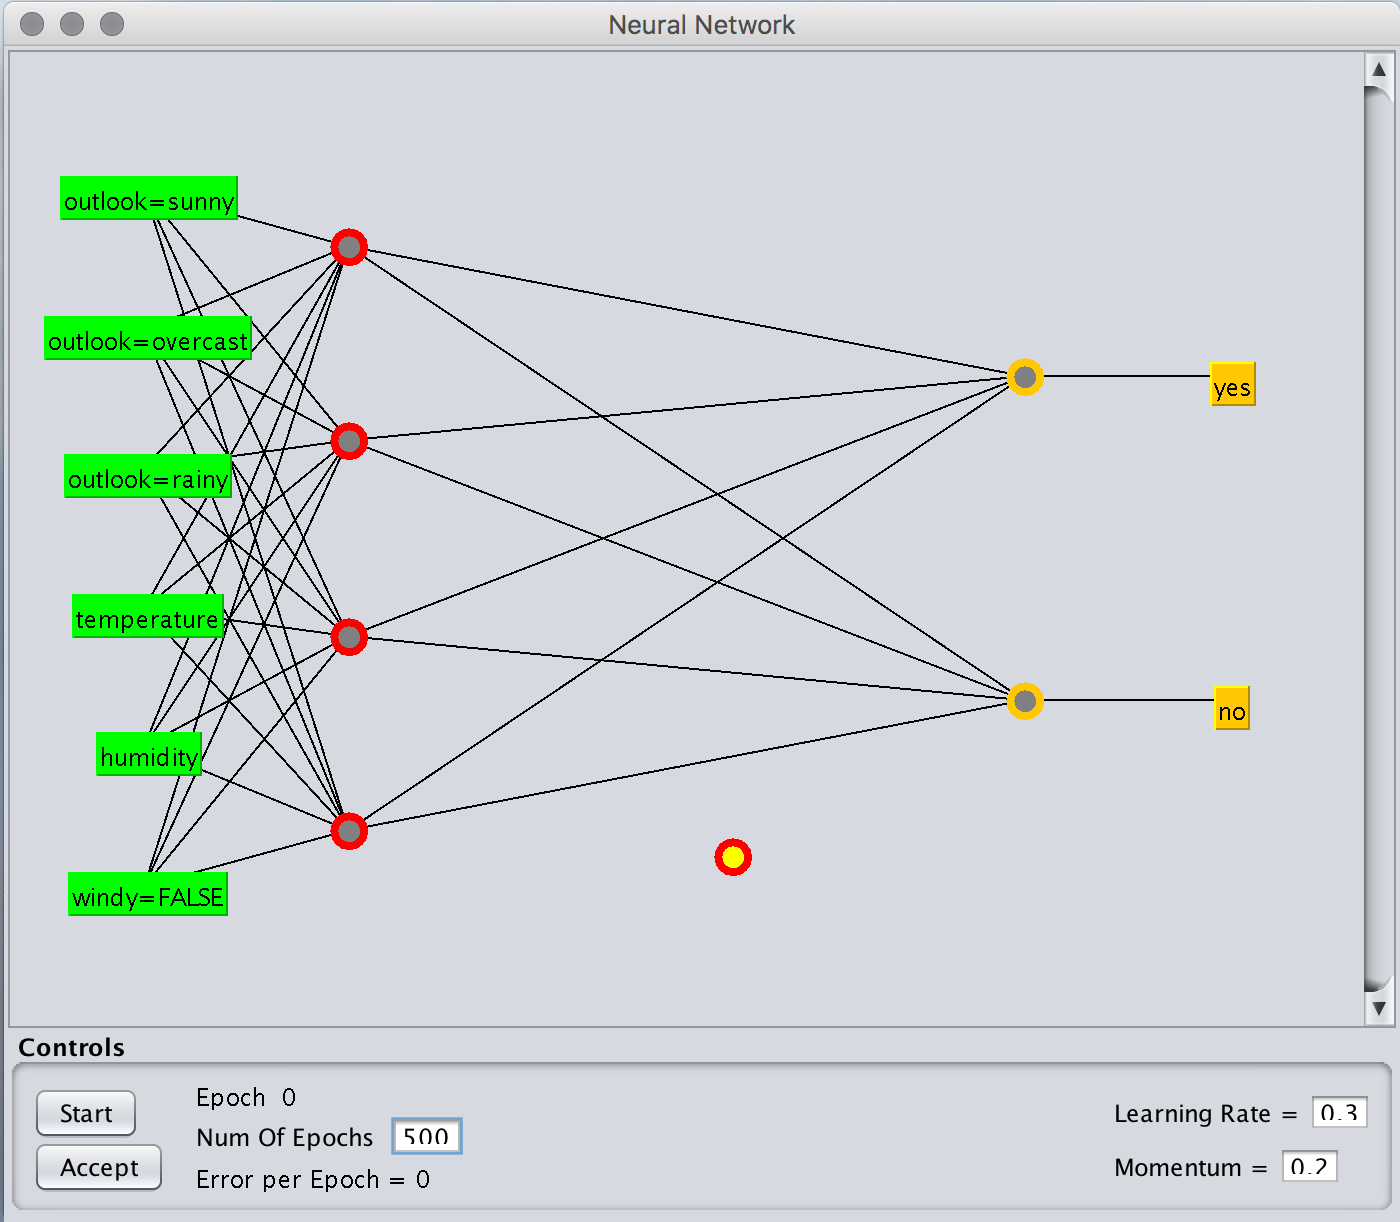
\includegraphics[width=0.75\textwidth]{images/B2_27a.png}}
\qquad
\subfloat[The finished network with two hidden layers.]{\label{subfig:mlp_editor_2}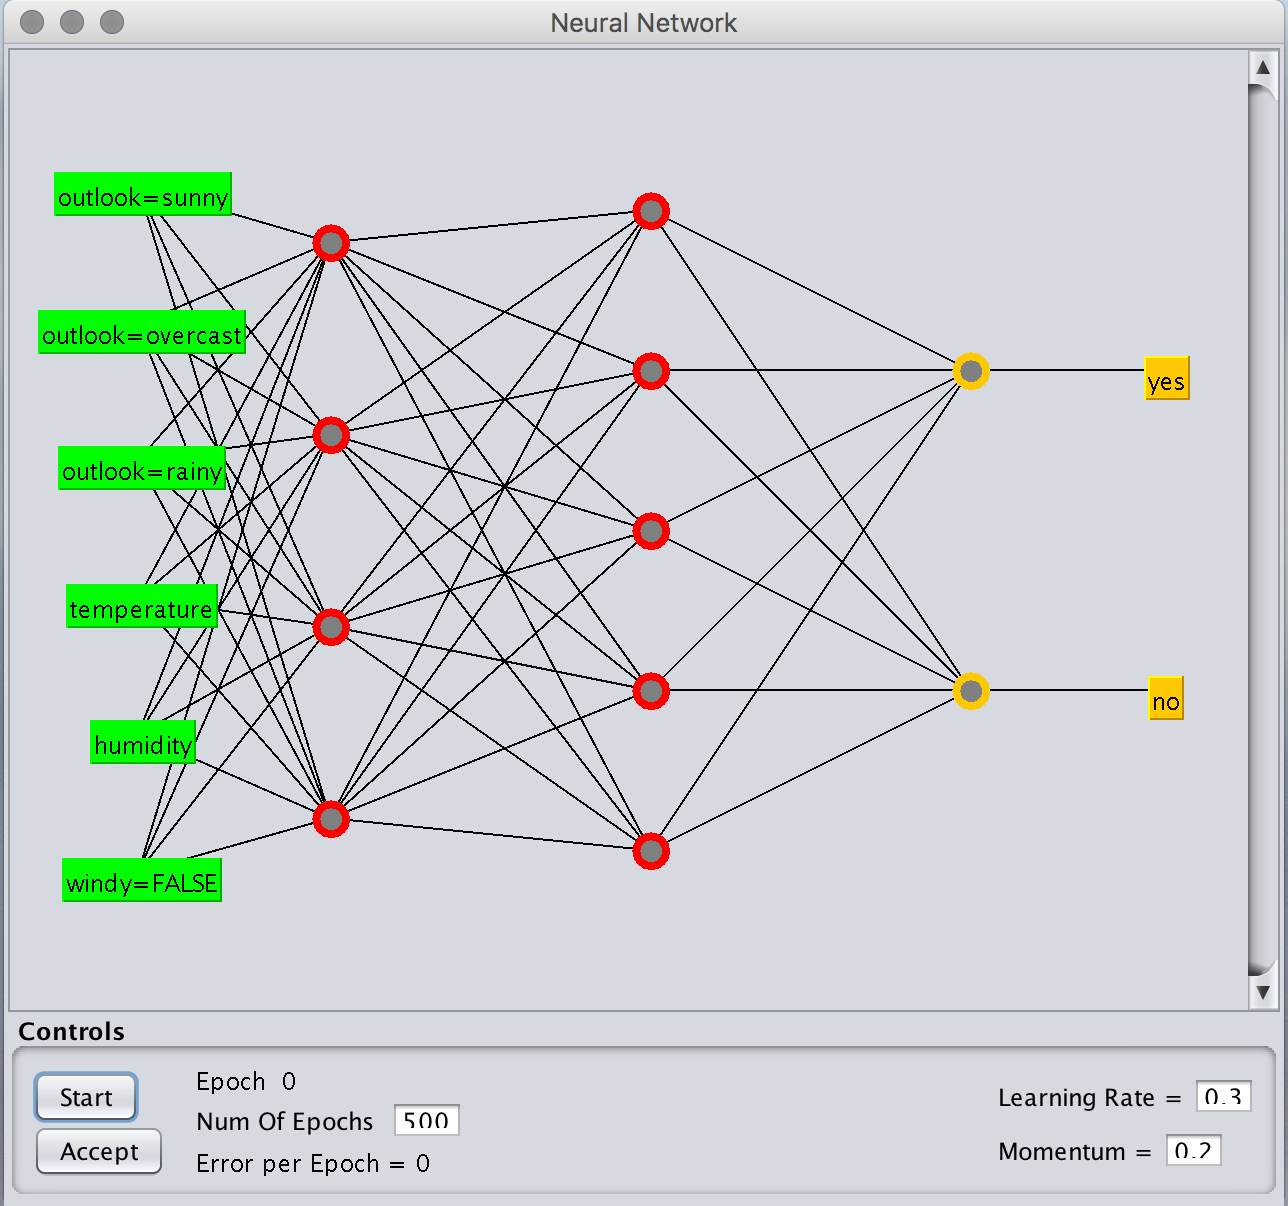
\includegraphics[width=0.75\textwidth]{images/B2_27b.png}}
\caption{\label{fig:mlp_editor}Using WEKA's neural-network graphical user interface.}
\end{figure}

\textit{MultilayerPerceptron} is a neural network that is trained using
back propagation. Although listed under functions, it differs from the
other schemes because it has its own user interface. If you load up
the numeric version of the weather data, invoke
\textit{MultilayerPerceptron}, set \textit{GUI} to \textit{True} in
its object editor, and run the network by clicking \textit{Start} on
the \textit{Classify} panel, the diagram in
Figure~\ref{fig:mlp_editor} appears in a separate window. This network
has three layers: an input layer on the left with one rectangular box
for each attribute (colored green); a hidden layer next to it (red) to
which all the input nodes are connected; and an output layer at the
right (orange). The labels at the far right show the classes that the
output nodes represent. Output nodes for numeric classes are
automatically converted to unthresholded linear units.

Before clicking \textit{Start} to run the network, you can alter its
structure by adding nodes and connections. Nodes can be selected or
deselected. All six nodes in the hidden and output layers in
Figure~\ref{fig:mlp_editor} are deselected, indicated by the gray
color of their center. To select a node, simply click on it. This
changes the color of its center from gray to bright yellow. To
deselect a node, right-click in an empty space. To add a node, ensure
that none is selected and left-click anywhere in the panel; the new
node will be selected automatically. In Figure~\ref{fig:mlp_editor}, a
new node has been added at the lower center. To connect two nodes,
select the start node and then click on the end one. If several start
nodes are selected, they are all connected to the end node. If you
click in empty space instead, a new node is created as the end
node. Notice that connections are directional (although the directions
are not shown). The start nodes remain selected; thus you can add an
entire hidden layer with just a few clicks, as shown in
Figure~\ref{subfig:mlp_editor_2}. To remove a node, ensure that no nodes
are selected and right-click it; this also removes all connections to
it. To remove a single connection, select one node and right-click the
node at the other end.

As well as configuring the structure of the network, you can control
the learning rate, the momentum, and the number of passes that will be
taken through the data, called \textit{epochs}. The network begins to
train when you click {\em Start}, and a running indication of the epoch and
the error for that epoch is shown at the lower left of the panel in
Figure~\ref{fig:mlp_editor}. Note that the error is based on a network
that changes as the value is computed. For numeric classes the error
value depends on whether the class is normalized. The network stops
when the specified number of epochs is reached, at which point you can
accept the result or increase the desired number of epochs and press
\textit{Start} again to continue training.

\textit{MultilayerPerceptron} need not be run through the graphical
interface. Several parameters can be set from the object editor to
control its operation. If you are using the graphical interface they
govern the initial network structure, which you can override
interactively. With \textit{autoBuild} set, hidden layers are added
and connected up. The default is to have the one hidden layer shown in
Figure~\ref{subfig:mlp_editor_1}, but without \textit{autoBuild} this
would not appear and there would be no connections. The
\textit{hiddenLayers} parameter defines what hidden layers are present
and how many nodes each one contains. Figure~\ref{subfig:mlp_editor_1}
is generated by a value of 4 (one hidden layer with four nodes), and
although~\ref{subfig:mlp_editor_2} was created by adding nodes
interactively, it could have been generated by setting
\textit{hiddenLayers} to \textit{4,5} (one hidden layer with four
nodes and another with five). The value is a comma-separated list of
integers; \textit{0} gives no hidden layers. Furthermore, there are
predefined values that can be used instead of integers: $i$ is the
number of attributes, $o$ the number of class values, $a$ the average
of the two, and $t$ their sum. The default, $a$, was used to generate
Figure~\ref{subfig:mlp_editor_1}.

The options \textit{learningRate} and \textit{momentum} set values
for these parameters, which can be overridden in the graphical
interface. A \textit{decay} parameter causes the learning rate to
decrease with time: it divides the starting value by the epoch number
to obtain the current rate. This sometimes improves performance and
may stop the network from diverging. The reset parameter automatically
resets the network with a lower learning rate and begins training
again if it is diverging from the answer (this option is only
available if the graphical interface is not used).

The \textit{trainingTime} parameter sets the number of training
epochs. Alternatively, a percentage of the data can be set aside for
validation (using \textit{validationSetSize}): then training continues
until performance on the validation set starts to deteriorate
consistently---or until the specified number of epochs is reached. If
the percentage is set to zero, no validation set is used. The
\textit{validationThreshold} parameter determines how many consecutive
times the validation set error can deteriorate before training is
stopped.

The \textit{NominalToBinaryFilter} filter is specified by default in
the \textit{MultilayerPerceptron} object editor; turning it off may
improve performance on data in which the nominal attributes are really
ordinal. The attributes can be normalized (with
\textit{normalizeAttributes}), and a numeric class can be normalized
too (with \textit{normalizeNumericClass}). Both may improve
performance; these options are turned on by default.

\subsection{Lazy classifiers}

Lazy learners store the training instances and do no real work until
classification time. The simplest lazy learner is the
\textit{k}-nearest-neighbor classifier, which is implemented by
\textit{IBk}. A variety of different search algorithms can be used to
speed up the task of finding the nearest neighbors. A linear search is
the default, but other options include kD-trees, ball trees and
so-called ``cover trees'' (Beygelzimer et al., 2006). The distance
function used is a parameter of the search method. The default is the
same as for \textit{IB1}, that is, the Euclidean distance; other
options include Chebyshev, Manhattan and Minkowski distances. The
number of nearest neighbors (default $k$ = 1) can be specified
explicitly in the object editor or determined automatically using
leave-one-out cross-validation, subject to an upper limit given by the
specified value. Predictions from more than one neighbor can be
weighted according to their distance from the test instance, and two
different formulas are implemented for converting the distance into a
weight. The number of training instances kept by the classifier can be
restricted by setting the window size option. As new training
instances are added, the oldest ones are removed to maintain the
number of training instances at this size \textit{KStar} is a
nearest-neighbor method with generalized distance function based on
transformations, discussed in Chapter 7 of the book.

\textit{LWL} is a general algorithm for locally weighted learning. It
assigns weights using an instance-based method and builds a classifier
from the weighted instances. The classifier is selected in
\textit{LWL's} object editor: a good choice is naive Bayes or logistic
regression for classification problems and linear regression for
regression problems. You can set the number of neighbors used, which
determines the kernel bandwidth, and the kernel shape to use for
weighting---linear, inverse, or Gaussian. Attribute normalization is
turned on by default.

\subsection{Miscellaneous classifiers}

The ``Misc.'' category includes just two classifiers, unless further
corresponding WEKA packages have been
installed. \textit{SerializedClassifier} loads a model that has been
serialized to a file and uses it for prediction. Providing a new
training dataset has no effect, because it encapsulates a static
model. Similarly, performing cross-validation using
\textit{SerializedClassifier} makes little
sense. \textit{InputMappedClassifier} wraps a base classifier (or
model that has been serialized to a file) and constructs a mapping
between the attributes present in the incoming test data and those
that were seen when the model was trained. Values for attributes
present in the test data but not in the training data are simply
ignored. Values for attributes present at training time but not
present in the test data receive missing values. Similarly, missing
values are used for incoming nominal values not seen during training.

\subsection{Metalearning algorithms}

Metalearning algorithms take classifiers and turn them into more
powerful learners. One parameter specifies the base classifier(s); others
specify the number of iterations for iterative schemes such as bagging
and boosting and an initial seed for the random number generator. We
already met \textit{FilteredClassifier} in
Section~\ref{subsection:supervised_filters}: it runs a classifier on
data that has been passed through a filter, which is a parameter. The
filter's own parameters are based exclusively on the training data,
which is the appropriate way to apply a supervised filter to test
data.

\subsubsection{Bagging and randomization}

\textit{Bagging} bags a classifier to reduce variance. This
implementation works for both classification and regression, depending
on the base learner. In the case of classification, predictions are
generated by averaging probability estimates, not by voting. One
parameter is the size of the bags as a percentage of the training
set. Another is whether to calculate the out-of-bag error, which gives
the average error of the ensemble members (Breiman 2001).

\textit{RandomCommittee} is even simpler: it builds an ensemble of
base classifiers and averages their predictions. Each one is based on
the same data but uses a different random number seed. This only makes
sense if the base classifier is randomized; otherwise, all classifiers
would be the same.

\textit{RandomSubSpace} builds an ensemble of classifiers, each
trained using a randomly selected subset of the input
attributes. Aside from the number of iterations and random seed to
use, it provides a parameter to control the size of the attribute
subsets. \textit{RotationForest} implements the rotation forest
ensemble learner. Although the classic paper on rotation forests,
Rodriguez et al. (2006), uses random subspaces and principal
components to create an ensemble of decision trees, WEKA's
implementation allows the base classifier to be any classification or
regression scheme. The principal components transformation is
performed by WEKA's filter of the same name. \textit{RotationForest}
can be configured to use other projections such as random projections
or partial least squares. Other parameters control the size of the
subspaces and the number of instances that are input to the projection
filter.

\subsubsection{Boosting}

\textit{AdaBoostM1} implements the classic boosting algorithm. It can
be accelerated by specifying a threshold for weight
pruning. AdaBoostM1 resamples if the base classifier cannot handle
weighted instances (you can also force resampling anyway).

Whereas \textit{AdaBoostM1} only applies to nominal classes,
\textit{AdditiveRegression} enhances the performance of a regression
learner. There are two parameters: shrinkage, which governs the
learning rate, and the maximum number of models to generate. If the
latter is infinite, work continues until the error stops decreasing.

\textit{LogitBoost} performs additive logistic regression. Like
\textit{AdaBoostM1}, it can be accelerated by specifying a threshold
for weight pruning. The appropriate number of iterations can be
determined using internal cross-validation; there is a shrinkage
parameter that can be tuned to prevent overfitting; and you can choose
resampling instead of reweighting.

\subsubsection{Combining classifiers}

\textit{Vote} provides a baseline method for combining
classifiers. The default scheme is to average their probability
estimates or numeric predictions, for classification and regression
respectively. Other combination schemes are available, for example,
using majority voting for classification.

{\em Stacking} combines classifiers using stacking for both classification
and regression problems. You specify the base classifiers, the
metalearner, and the number of cross-validation folds.

\subsubsection{Cost-sensitive learning}

There is one metalearner, called \textit{CostSensitiveLearning}, for
cost-sensitive learning. The cost matrix can be supplied as a
parameter or loaded from a file in the directory set by the
\textit{onDemandDirectory} property, named by the relation name and
with the extension {\em cost}. \textit{CostSensitiveClassifier} either
reweights training instances according to the total cost assigned to
each class or predicts the class with the minimum expected
misclassification cost rather than the most likely one.

\subsubsection{Optimizing performance}

Five metalearners use the wrapper technique to optimize the base
classifier's performance. \textit{AttributeSelectedClassifier} selects
attributes, reducing the data's dimensionality before passing it to
the classifier. You can choose the attribute evaluator and search
method as in the {\em Select attributes} panel described in
Section~\ref{section:exploring_the_explorer}. \textit{CVParameterSelection}
optimizes performance by using cross-validation to select
parameters. For each parameter you give a string containing its lower
and upper bounds and the desired number of increments. For example, to
vary parameter --P from 1 to 10 in increments of 1, use\newline

P 1 10 10\newline

The number of cross-validation folds to be used can be specified.

\textit{MultiScheme} selects a classifier to use from among several by
using either the resubstitution error or cross-validation on the
training data. Performance is measured using percentage correct in the
case of classification and mean squared error for regression.

\textit{IterativeClassifierOptimizer} optimizes the number of iterations
performed by iterative classifiers, such as boosting methods, using
cross-validation on the training data. Performance can be measured
using any of the metrics described in Chapter 5 of the book. The user can specify
parameters such as how many cross-validation folds to use, how many
iterations to look ahead in order to find a better solution, and how
often to perform the evaluation (if evaluation of every iteration is
proving too time consuming).

The fifth metalearner, \textit{ThresholdSelector}, optimizes one of a
number of different evaluation metrics, including F-measure,
precision, recall, accuracy and true positive rate, by selecting a
probability threshold on the classifier's output. Performance can
measured on the training data, on a holdout set, or by
cross-validation. The probabilities returned by the base learner can
be rescaled into the full range [0,1], which is useful if the scheme's
probabilities are restricted to a narrow subrange. The metalearner can
be applied to multiclass problems by specifying the class value for
which the optimization is performed as

\begin{enumerate}
\item The first class value.
\item The second class value.
\item Whichever value is least frequent.
\item Whichever value is most frequent.
\item The first class named \textit{yes}, \textit{pos(itive)}, or \textit{1}.
\end{enumerate}

\subsubsection{Retargeting classifiers for different tasks}

Three metalearners adapt learners designed for one kind of task to
another. \textit{ClassificationViaRegression} performs classification
using a regression method by binarizing the class and building a
regression model for each value. \textit{RegressionByDiscretization}
is a regression scheme that discretizes the class attribute into a
specified number of bins using equal-width discretization and then
employs a classifier. The predictions are the weighted average of the
mean class value for each discretized interval, with weights based on
the predicted probabilities for the intervals.

\textit{MultiClassClassifier} handles multiclass problems with
two-class classifiers using any of these methods:

\begin{enumerate}
\item One versus all the rest.
\item Pairwise classification using voting to predict.
\item Exhaustive error-correcting codes.
\item Randomly selected error-correcting codes.
\end{enumerate}

Random code vectors are known to have good error-correcting
properties: a parameter specifies the length of the code vector as a
factor that is multiplied by the number of classes in the data. For
pairwise classification, pairwise coupling of probability estimates
can be turned on.

\section{Clustering algorithms}

The {\em Cluster} panel provides access to clustering
algorithms. \textit{Cobweb} and \textit{SimpleKMeans} are described in
Chapter 4 of the book; \textit{EM} is described in Chapter 9. For the
\textit{EM} implementation you can specify how many clusters to
generate, or the algorithm can decide by cross-validating the loglikelihood---in which
case the number of folds is fixed at 10 (unless there are fewer than
10 training instances). You can specify the maximum number of
iterations and set the minimum allowable standard deviation for the
normal density calculation. Clusters are Gaussian distributions with
diagonal covariance matrices. \textit{SimpleKMeans} clusters data
using \textit{k}-means; the number of clusters is specified by a
parameter. The user can choose between the Euclidean and Manhattan
distance metrics. In the latter case the algorithm is actually
\textit{k}-medians instead \textit{k}-means, and the centroids are
based on medians rather than means in order to minimize the
within-cluster distance function.

\begin{figure}[!tp]
%\centering
\begin{mdframed}[innermargin=-1.0cm]
\begin{Verbatim}[fontsize=\footnotesize]
=== Run information ===

Scheme:       weka.clusterers.SimpleKMeans -init 0 -max-candidates 100
              -periodic-pruning 10000 -min-density 2.0 -t1 -1.25 -t2 -1.0 -N 2 
              -A ``weka.core.EuclideanDistance -R first-last'' -I 500 
              -num-slots 1 -S 10
Relation:     weather
Instances:    14
Attributes:   5
              outlook
              temperature
              humidity
              windy
              play
Test mode:    evaluate on training data


=== Clustering model (full training set) ===


kMeans
======

Number of iterations: 3
Within cluster sum of squared errors: 16.237456311387238

Initial starting points (random):

Cluster 0: rainy,75,80,FALSE,yes
Cluster 1: overcast,64,65,TRUE,yes

Missing values globally replaced with mean/mode

Final cluster centroids:
                           Cluster#
Attribute      Full Data          0          1
                  (14.0)      (9.0)      (5.0)
==============================================
outlook            sunny      sunny   overcast
temperature      73.5714    75.8889       69.4
humidity         81.6429    84.1111       77.2
windy              FALSE      FALSE       TRUE
play                 yes        yes        yes




Time taken to build model (full training data) : 0 seconds

=== Model and evaluation on training set ===

Clustered Instances

0       9 ( 64%)
1       5 ( 36%)
\end{Verbatim}
\end{mdframed}
\caption{\label{fig:kmeans_output}Output of \textit{SimpleKMeans} for the weather data.}
\end{figure}

Figure~\ref{fig:kmeans_output} shows the output of \textit{SimpleKMeans}
for the weather data, with default options: two clusters and Euclidean
distance. The result of clustering is shown as a table whose rows are
attribute names and whose columns correspond to the cluster centroids;
an additional cluster at the beginning shows the entire data set. The
number of instances in each cluster appears in parentheses at the top
of its column. Each table entry is either the mean (numeric attribute)
or mode (nominal attribute) of the corresponding attribute for the
cluster in that column; users can choose to show standard deviations
(numeric attribute) and frequency counts (nominal attributes) as
well. The bottom of the output shows the result of applying the
learned clustering model. In this case, it assigned each training
instance to one of the clusters, showing the same result as the
parenthetical numbers at the top of each column. An alternative is to
use a separate test set or a percentage split of the training data, in
which case the figures would be different.

\begin{figure}[!tp]
%\centering
\begin{mdframed}[innermargin=-1.0cm]
\begin{Verbatim}[fontsize=\footnotesize]
=== Run information ===

Scheme:       weka.clusterers.EM -I 100 -N 2 -X 10 -max -1 
              -ll-cv 1.0E-6 -ll-iter 1.0E-6 -M 1.0E-6 -K 10 
              -num-slots 1 -S 100
Relation:     weather
Instances:    14
Attributes:   5
              outlook
              temperature
              humidity
              windy
              play
Test mode:    evaluate on training data


=== Clustering model (full training set) ===


EM
==

Number of clusters: 2
Number of iterations performed: 7


              Cluster
Attribute           0       1
               (0.35)  (0.65)
==============================
outlook
  sunny         3.8732  3.1268
  overcast      1.7746  4.2254
  rainy         2.1889  4.8111
  [total]       7.8368 12.1632
temperature
  mean         76.9173 71.8054
  std. dev.     5.8302  5.8566

humidity
  mean         90.1132 77.1719
  std. dev.     3.8066  9.1962

windy
  TRUE            3.14    4.86
  FALSE         3.6967  6.3033
  [total]       6.8368 11.1632
play
  yes           2.1227  8.8773
  no            4.7141  2.2859
  [total]       6.8368 11.1632


Time taken to build model (full training data) : 0 seconds

=== Model and evaluation on training set ===

Clustered Instances

0       4 ( 29%)
1      10 ( 71%)


Log likelihood: -9.13037
\end{Verbatim}
\end{mdframed}
\caption{\label{fig:em_output}Output of \textit{EM} for the weather data.}
\end{figure}

Figure 2.29 shows the output of \textit{EM} for the same data, with
the number of clusters set to two. Although there is no notion of the
number of instances in each cluster, the columns are again headed by
its prior probability in parentheses. The table entries show the
parameters of normal distributions for numeric attributes or frequency
counts for the values of nominal attributes---and here the fractional
count values reveal the ``soft'' nature of the clusters produced by the
EM algorithm, in that any instance can be split between several
clusters. At the bottom the loglikelihood of the model (again with
respect to the training data) is shown, as well as the number of
instances assigned to each cluster when the learned model is applied
to the data as a classifier.

\textit{Cobweb} implements both the Cobweb algorithm for nominal
attributes and the Classit algorithm for numeric attributes. The
ordering and priority of the merging and splitting operators differs
from the original Cobweb and Classit papers (where it is somewhat
ambiguous). This implementation always compares four different ways of
treating a new instance and chooses the best: adding it to the best
host, making it into a new leaf, merging the two best hosts and adding
it to the merged node, and splitting the best host and adding it to
one of the splits. \textit{Acuity} and \textit{cutoff} are parameters.

\textit{HierarchicalClusterer} implements agglomerative (bottom-up)
generation of hierarchical clusters (Section 6.8 of the book). Several
different link types, which are ways of measuring the distance between
clusters, are available as options.

\textit{FarthestFirst} implements the farthest-first traversal
algorithm of Hochbaum and Shmoys (1985), cited by Sanjoy Dasgupta
(2002); a fast, simple, approximate clusterer modeled on
$k$-means. \textit{MakeDensityBasedClusterer} is a metaclusterer that
wraps a clustering algorithm to make it return a probability
distribution and density. To each cluster and attribute it fits a
discrete distribution or a symmetric normal distribution (whose
minimum standard deviation is a parameter).

\textit{Canopy} implements the canopy clustering algorithm algorithm
of McCallum, Nigam and Ungar (2000). Canopy clustering is often used
as an initialization strategy for \textit{k}-means or as a fast
approximate clustering method for use on large datasets, where
applying another algorithm directly might be impractical. The
algorithm partitions the input data into proximity regions (canopies)
in the form of hyperspheres defined by a loose distance, \textit{T1},
from the region's center. A second tight distance, \textit{T2} (where
$T2 < T1$), is used to control how many canopies are formed by the
algorithm. At most two passes over the data are required. The first
pass creates the canopies, and it starts by choosing one instance at
random to form the center of the first canopy. Following this, each of
the remaining instances are considered in turn, by computing its
distance to the center of each existing canopy. If a given instance is
outside the T2 distance to all canopies then it forms a new canopy,
otherwise it is discarded. The second pass over the data assigns
instances to canopies and makes use of the loose \textit{T1}
distance. Because canopies can overlap according to \textit{T1}
distance, it is possible for a given instance to belong to more than
one canopy.

\section{Association rule learners}

WEKA has three association rule learners. \textit{Apriori} implements
the Apriori algorithm. It starts with a minimum support of 100\% of
the data items and decreases this in steps of 5\% until there are at
least 10 rules with the required minimum confidence of 0.9 or until
the support has reached a lower bound of 10\%, whichever occurs
first. (These default values can be changed.) There are four
alternative metrics for ranking rules: \textit{Confidence}, which is
the proportion of the examples covered by the premise that are also
covered by the consequent; \textit{Lift}, which is determined by
dividing the confidence by the support; \textit{Leverage}, which is
the proportion of additional examples covered by both the premise and
the consequent beyond those expected if the premise and consequent
were statistically independent; and \textit{Conviction}, a measure defined by
Brin et al. (1997). You can also specify a significance level, and
rules will be tested for significance at this level. Apriori has an
option to limit the rules found to those that contain just the value
of a single attribute in the consequence of the rule. Such rules are
called ``class'' association rules---i.e., classification rules.

In order to process market-basket data with Apriori, where we are
interested in knowing (from the items present in shoppers' baskets)
which items are purchased together, it is necessary to encode the
input ARFF data in a specific way. In particular, since we are not
interested in co-occurrence of items not present in shopping baskets,
the attributes corresponding to items should be declared as
single-valued nominal ones in the ARFF file. Missing values can be
used to indicate the absence of an item from a shopping basket.

\textit{FPGrowth} implements the frequent pattern tree mining
algorithm. Being designed for market-basket data, Apriori's special
encoding for this type of data is not implemented here. All attributes
are expected to be binary nominal ones, and the user can specify which
of the two values is to be treated as positive, i.e., indicates
presence in the basket (the default is to use the second
value). FPGrowth can operate on either standard or sparse
instances. Most of its options are the same as for Apriori. It finds
the requested number of rules in the same way---by iteratively
decreasing the minimum support. Optionally, the user can have FPGrowth
find all the rules that meet the lower bound for the minimum support
and the minimum value set for the ranking metric (confidence, lift,
leverage or conviction).

\textit{FilteredAssociator} allows the data to be passed through a
filter before it reaches an associator. Both the filter and the base
associator are options that the user can configure.

\section{Attribute selection}

\begin{figure}[!th]
\centering
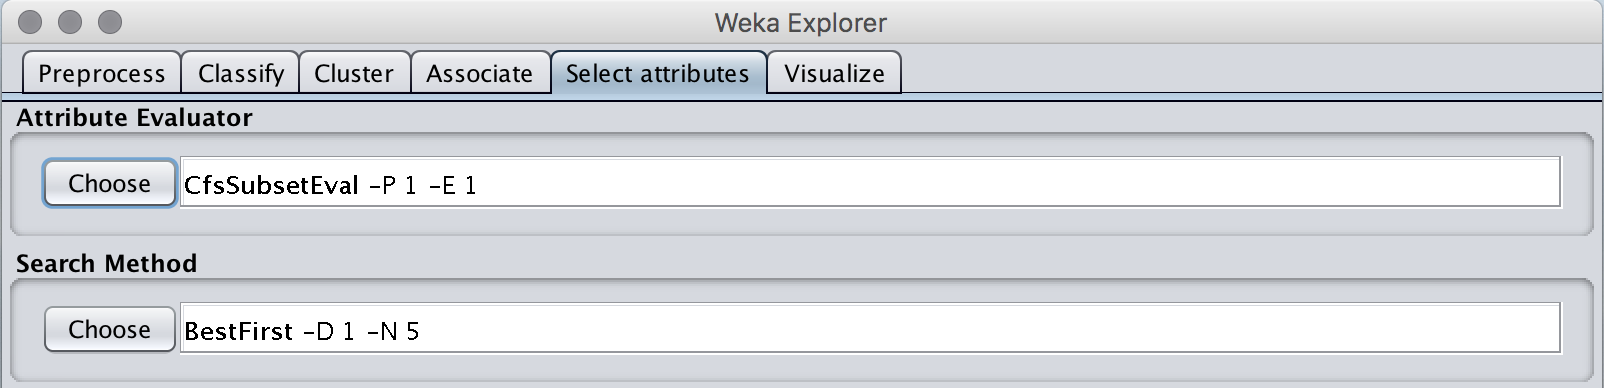
\includegraphics[width=0.9\textwidth]{images/B2_30.png}
\caption{Attribute selection: specifying an evaluator and a search method.}
\label{fig:att_selection_config}
\end{figure}

Figure~\ref{fig:att_selection_config} shows that part of WEKA's
attribute selection panel where you specify the attribute evaluator
and search method. Attribute selection is normally done by searching
the space of attribute subsets, evaluating each one. A potentially
faster but less accurate approach is to evaluate the attributes
individually and sort them, discarding attributes that fall below a
chosen cut-off point.

\subsection{Attribute subset evaluators}

Subset evaluators take a subset of attributes and return a numerical
measure that guides the search. They are configured like any other
WEKA object. \textit{CfsSubsetEval} assesses the predictive ability of
each attribute individually and the degree of redundancy among them,
preferring sets of attributes that are highly correlated with the
class but with low intercorrelation. An option iteratively adds
attributes that have the highest correlation with the class, provided
that the set does not already contain an attribute whose correlation
with the attribute in question is even higher. Missing can be treated
as a separate value, or its counts can be distributed among other
values in proportion to their frequency.

Whereas \textit{CfsSubsetEval} is a filter method of attribute
selection, \textit{WrapperSubsetEval} implements a wrapper
method. \textit{WrapperSubsetEval} uses a classifier to evaluate
attribute set and employs cross-validation to estimate the accuracy of
the learning scheme for each set.

\subsection{Single-attribute evaluators}

Single-attribute evaluators are used with the \textit{Ranker} search
method to generate a ranked list from which \textit{Ranker} discards a
given number (explained in the next
subsection). \textit{ReliefFAttributeEval} is instance-based: it
samples instances randomly and checks neighboring instances of the
same and different classes. It operates on discrete and continuous
class data. Parameters specify the number of instances to sample, the
number of neighbors to check, whether to weight neighbors by distance,
and an exponential function that governs how rapidly weights decay
with distance.

\textit{InfoGainAttributeEval} evaluates attributes by measuring their
information gain with respect to the class. It discretizes numeric
attributes first using the MDL-based discretization method (it can be
set to binarize them instead). This method, along with the next three,
can treat missing as a separate value or distribute the counts among
other values in proportion to their
frequency. \textit{ChiSquaredAttributeEval} evaluates attributes by
computing the chi-squared statistic with respect to the
class. GainRatioAttributeEval evaluates attributes by measuring their
gain ratio with respect to the
class. \textit{SymmetricalUncertAttributeEval} evaluates an attribute
by measuring its symmetrical uncertainty with respect to the class.

\textit{OneRAttributeEval} uses the simple accuracy measure adopted by
the \textit{OneR} classifier. It can use the training data for
evaluation, as OneR does, or it can apply internal cross-validation:
the number of folds is a parameter. It adopts \textit{OneR's} simple
discretization method: the minimum bucket size is a parameter.

Unlike other single-attribute evaluators, \textit{PrincipalComponents}
transforms the set of attributes. The new attributes are ranked in
order of their eigenvalues. Optionally, a subset is selected by
choosing sufficient eigenvectors to account for a given proportion of
the variance (95\% by default). Finally, the reduced data can be
transformed back to the original space.

\subsection{Search methods}

Search methods traverse the attribute space to find a good
subset. Quality is measured by the chosen attribute subset
evaluator. Each search method can be configured with WEKA's object
editor. \textit{BestFirst} performs greedy hill climbing with
backtracking; you can specify how many consecutive nonimproving nodes
must be encountered before the system backtracks. It can search
forward from the empty set of attributes, backward from the full set,
or start at an intermediate point (specified by a list of attribute
indexes) and search in both directions by considering all possible
single-attribute additions and deletions. Subsets that have been
evaluated are cached for efficiency; the cache size is a parameter.

\textit{GreedyStepwise} searches greedily through the space of
attribute subsets. Like \textit{BestFirst}, it may progress forward
from the empty set or backward from the full set. Unlike
\textit{BestFirst}, it does not backtrack but terminates as soon as
adding or deleting the best remaining attribute decreases the
evaluation metric. In an alternative mode, it ranks attributes by
traversing the space from empty to full (or vice versa) and recording
the order in which attributes are selected. You can specify the number
of attributes to retain or set a threshold below which attributes are
discarded.

Finally we describe \textit{Ranker}, which as noted earlier is not a
search method for attribute subsets but a ranking scheme for
individual attributes. It sorts attributes by their individual
evaluations and must be used in conjunction with one of the
single-attribute evaluators---not an attribute subset
evaluator. \textit{Ranker} not only ranks attributes but also performs
attribute selection by removing the lower-ranking ones. You can set a
cut-off threshold below which attributes are discarded, or specify how
many attributes to retain. You can specify certain attributes that
must be retained regardless of their rank.

